\documentclass[a4paper,10pt]{report}

\usepackage{graphicx}
\usepackage{hyperref}
\usepackage{amsmath}
\usepackage{amssymb}
\usepackage{xspace}
\pagestyle{headings}
%\usepackage[margin=1.2in]{geometry}
\usepackage[left=2cm, right=2cm, top=2.5cm, bottom=2cm]{geometry}
\usepackage{float}
\restylefloat{table}
\usepackage{listings}
\usepackage{color}
\definecolor{gray}{rgb}{0.4,0.4,0.4}
\definecolor{darkblue}{rgb}{0.0,0.0,0.58}
\definecolor{attributeColor}{rgb}{0.96,0.517,0.29}
\definecolor{darkgreen}{rgb}{0,.392,0}
\definecolor{stringColor}{rgb}{0.6,0.2,0}
\usepackage{array,multirow}
\usepackage{longtable}
\usepackage{cleveref}
\usepackage{bbding}
\crefname{section}{�}{��}
\Crefname{section}{�}{��}
\usepackage[utf8]{inputenc}
\usepackage{tablefootnote}

\newcommand{\myStartLine}{\par
  \kern8pt % space above the rules
  \hrule height 0.5pt
  \kern3pt % space below the rules
}
\newcommand{\myEndLine}{\par
  \kern3pt % space above the rules
  \hrule height 1.5pt
  \kern12pt % space below the rules
}

%\lstset{
%  basicstyle=\ttfamily,
%  columns=fullflexible,
%  showstringspaces=false,
%  commentstyle=\color{gray}\upshape
%  numbers=left,
%%  frame = single, 
%%  stepnumber=5
%}

\newcommand{\HRule}{\rule{\linewidth}{0.5mm}}

\lstdefinelanguage{XML}
{
  basicstyle=\ttfamily\footnotesize,
  morestring=[b]",
  morestring=[s]{>}{<},
  moredelim=[s][\bfseries\color{darkblue}]{<}{\ },
  moredelim=[s][\bfseries\color{darkblue}]{</}{>},
  moredelim=[l][\bfseries\color{darkblue}]{/>},
  moredelim=[l][\bfseries\color{darkblue}]{>},
  morecomment=[s]{<?}{?>},
  morecomment=[s]{<![CDATA[}{]]>},
  moredelim=[s][\bfseries\color{darkgreen}]{<!--}{-->},
  commentstyle=\color{darkgreen},
  stringstyle=\color{stringColor},
  identifierstyle=\color{red},
  keywordstyle=\color{attributeColor},
  morekeywords={oid,columnId,columnIdRef,symbId,symbolType,op,columnNum,columnType,
  valueType,inputTarget,blkId,blkIdRef,symbIdRef,xmlns,version,type,VariableMapping,
  IndividualMapping,schemaLocation,xs,xsi,NONMEMdataSet,matrixType,opType,order,
  math,ct,ds,mdef,mstep,mml,un,name,definition,writtenVersion,id,inputType,oidRef,catId,
  length,default,vectorIndex,diagDefault,offDiagDefault,row,column,numbRows,numbCols,
  dataSymbol,modelSymbol,ordered,compartmentNo,compNo,ordered,linkFunction,varId,
  censoringType,dataSymbol,modelSymbol,MarkovOrder,deviationMatrixType,implementedBy} % list your attributes here
}

\lstdefinelanguage{MLXTRANcode} 
{
  basicstyle=\ttfamily\footnotesize,
  morestring=[b]",
  morestring=[s]{>}{<},
  moredelim=[s][\bfseries\color{darkblue}]{<}{\ },
  moredelim=[s][\bfseries\color{darkblue}]{</}{>},
  moredelim=[l][\bfseries\color{darkblue}]{/>},
  moredelim=[l][\bfseries\color{darkblue}]{>},
  morecomment=[s]{<?}{?>},
  morecomment=[s]{<!--}{-->},
  morecomment=[s]{<![CDATA[}{]]>},
  commentstyle=\color{darkgreen},
  stringstyle=\color{stringColor},
  identifierstyle=\color{black},
  keywordstyle=\color{attributeColor},
  morekeywords={dads} % list your attributes here
}

\lstdefinelanguage{NONMEMdataSet}
{
  basicstyle=\ttfamily\footnotesize,
  morestring=[b]",
  morestring=[s]{>}{<},
  moredelim=[s][\bfseries\color{darkblue}]{<}{\ },
  moredelim=[s][\bfseries\color{darkblue}]{</}{>},
  moredelim=[l][\bfseries\color{darkblue}]{/>},
  moredelim=[l][\bfseries\color{darkblue}]{>},
  morecomment=[s]{<?}{?>},
  morecomment=[s]{<!--}{-->},
  morecomment=[s]{<![CDATA[}{]]>},
  commentstyle=\color{darkgreen},
  stringstyle=\color{stringColor},
  identifierstyle=\color{black},
  keywordstyle=\color{attributeColor},
  morekeywords={kjkj} % list your attributes here
}


\newcommand{\cellml}{CellML\xspace}
\newcommand{\sbml}{SBML\xspace}
\newcommand{\sedml}{SED-ML\xspace}
\newcommand{\mathml}{MathML\xspace}
\newcommand{\uncertml}{UncertML\xspace}
\newcommand{\pml}{PharmML\xspace}
\newcommand{\pharmml}{PharmML\xspace}
\newcommand{\xelem}[1]{\texttt{<#1>}\index{XML Element!\texttt{<#1>}}}
\newcommand{\xatt}[1]{\texttt{#1}\index{XML Attribute!\texttt{#1}}}

\begin{document}

\begin{titlepage}
\begin{center}

% Upper part of the page. The '~' is needed because \\
% only works if a paragraph has started.

\includegraphics[width=0.35\textwidth]{./logo/ddmore_logo}~\\[1cm]

%\textsc{\LARGE }\\[1.5cm]
%
\textsc{\Large Internal Release}\\[0.5cm]

% Title
\HRule \\[0.4cm]
{ \huge \bfseries Extensions and changes in PharmML 0.4 \& 0.4.1 \\[0.4cm] }

\HRule \\[1.5cm]

% Author and supervisor
\begin{minipage}{0.5\textwidth}
\begin{flushleft} \large
\emph{Authors:}\\
Maciek J \textsc{Swat}\\
Sarala \textsc{Wimalaratne}\\
Niels Rode \textsc{Kristensen}
\end{flushleft}
\end{minipage}
\begin{minipage}{0.4\textwidth}
\begin{flushright} \large
\emph{with contributions from:} \\
Elodie \textsc{Plan} \\
Roberto \textsc{Bizzotto} \\
Marc \textsc{Lavielle} \\
Pascal \textsc{Girard} 
\end{flushright}
\end{minipage}



\vfill

% Bottom of the page
{\large \today}

\end{center}
\end{titlepage} 
	
%\maketitle

\tableofcontents


%%%%%%%%%%%%%%%%%%%%%%%%%%%%%%%%%%%%%%%%%%%%%%%%%%%%%%%%%%%%%%%%%%%%%%
\chapter{Overview}

This document describes extensions and changes in \pml compared to the
previously released version 0.3.1. It is not intended to serve as a proper specification. 
The next public release, due in M42, will come with a fully updated specification document.
The current document introduces the discrete data models, delay differential equations,
extended vector and matrix support and a few new language elements and other corrections/changes.
The appendix \ref{chapter:codeExamples} contains examples of implemented discrete 
data models.

\paragraph{Major extensions in version 0.4}
The following table summarises the changes described in detail in the following chapters.

\begin{center}
\begin{longtable}{lll}
\hline
\hline
\pml element 			&  version $\le$ 0.3.1 			& version 0.4 \\
or modelling aspect 		&							& \\
\hline
Discrete data models 	& \emph{not supported}			& \xelem{Discrete} with child elements such as {\color{red} \scshape{new}} \\
(see \textsection\ref{chapter:DDmodels}) &				& -- \xelem{CountData} with \xelem{CountVariable}, \\
					&							& \xelem{PreviousCountVariable}, \xelem{Dependance},\\
					&							& \xelem{IntensityParameter}, etc.  \\
					&							& and \xelem{PMF} with \xatt{linkFunction} attribute \\
					&							& -- \xelem{CategoricalData} with child elements \\
					&							& such as \xelem{ListOfCategories}, \xelem{CategoryVariable}, \\
					&							& \xelem{InitialStateVariable} (plus few other \\
					&							& variable elements), \xelem{ProbabilityAssignment} and \\
					&							& its child elements: \xelem{Probability},  \xelem{CurrentState}, \\
					&							& \xelem{PreviousState} and \xelem{Condition} \\
					&							& -- \xelem{TimeToEventData} with child elements \\
					&							& \xelem{EventVariable}, \xelem{HazardFunction}, \\
					&							& \xelem{SurvivalFunction}, \xelem{Censoring} and \\
					&							& \xelem{MaximumNumberEvents} \\
\hline
Delay differential equations & \emph{not supported}	& \xelem{Delay} and \xelem{History} {\color{red} \scshape{new}} \\
(DDE) (see \textsection\ref{sec:DDEs})	& 					& with child elements \\ 
					&							& -- \xelem{HistoryValue} and \\
					&							& -- \xelem{HistoryTime}  \\ 
\hline
Extended vector definition & basic support 		 	& \xelem{Vector} with a number of child elements such as\\
 (see \textsection\ref{subsec:vectorType})	&	& \xelem{VectorElements}, \xelem{VectorCell}, \\
					& 							& \xelem{VectorSegment} and attributes \xatt{default}, \xatt{length}  \\ 
\hline
Extended matrix definition & basic support 		 	& \xelem{Matrix} with a number of child elements such as\\
 (see \textsection\ref{subsec:matrixStructure})	& 	& \xelem{MatrixRow}, \xelem{MatrixCell}, \\
					& 							& \xelem{MatrixBlock} and attributes \xatt{matrixType}, \\
					&							& \xatt{diagDefault}, \xatt{offDiagDefault} and others  \\ 
\hline
\caption{Overview of major differences between versions 0.4 and 0.3.1}
\label{figTable:overviewTable}
\end{longtable}
\end{center}


\chapter{Discrete data models}
\label{chapter:DDmodels}

%%%%%%%%%%%%%%%%%%%%%%%%%%%%%%%%%%%%%%%%%%%%%%%%%%%%%%%%%%%%%%%%%%%%%%%
%\section{Discrete data models}
%\label{sec:DDmodels}
%

% INPUT
\section{Introduction}
\label{sec:intro_discreteModels}

%Before we decided to postpone the support for discrete models we had a structure in place to accommodate few different discrete model types. The information needed to support, see \ref{subsec:mi_discreteModels}, consists of couple extension to what we had already. Formulating discrete data models as GLM or GLMM is not mandatory anymore. This means that one doesn't need to define the \textit{link} function or to restrict the predictor to linear models which simplifies our task on PharmML side.

The aim of this chapter is to collect, to classify and to propose the schema for 
implementation of discrete data models in PharmML as used in pharmacometrics.

It contains the mathematical description of discrete data models, mainly based 
on \cite{LavielleBook:2014} along with so called \emph{minimal information} -- a set of model elements to be 
stored to allow lossless encoding of models in PharmML and any target tool. 
Moreover, either MLXTRAN or NMTRAN implementation, or both, are provided. 

The proposed PharmML schema has been validated using available use cases. 
More then 25 various models have been successfully implemented so far. Nevertheless,
more testing is required before the official release (M42).

\subsection{\xelem{ObservationModel} extensions}
The following Figure \ref{fig:observationModel} shows the classification of continuous and discrete 
data models as used in this document and the proposed \pml structure. 
\begin{itemize}
\item
Continuous data
\begin{itemize}
\item
usually described by the normal distribution.
\end{itemize}
\item
Discrete data
\begin{itemize}
\item
Count data -- non-negative integers -- described by the Poisson or a related distribution.
\item
Categorical data -- finite set of integer values, nominal or ordered -- described by the Bernoulli
or the categorical distribution. 
\item
Time-to-event data -- time until an event occurs, can be unique or repeated -- described by 
survival or hazard function.
\end{itemize}
\end{itemize}
\begin{figure}[htb!]
\centering
 \includegraphics[width=140mm]{pics/observationModelExtended}
\caption{Observation model for continuous and discrete data. The residual error model of continuous 
data is described by a continuous distribution (e.g. normal distribution), while the error distribution of 
discrete data is described by a discrete distribution (e.g. binomial for binary data).}
\label{fig:observationModel}
\end{figure}
The proposed structure of the discrete data models 
in PharmML is outlined in Section \ref{subsec:mi_discreteModels}.


\subsection{Model unrelated features}
By "model unrelated features" we mean element of models which are provided
to assist a particular tool in their interpretation and execution. It was argued on multiple 
occasions that PharmML should be tool-independent. The analysis of NM-TRAN codes 
for few typical discrete data models resulted in the observation that especially these 
models contain a number of features, which are strictly speaking not part of the 
mathematical formulation of the models. This is related e.g. to the lack of certain built-in 
function or other algorithms specific to discrete data handling in NONMEM. The next few paragraphs 
deal with NONMEM specific approximations, coding tricks and simulation methods as applied 
in the case of discrete data models.  

\paragraph{Approximations}
Compared to MLXTRAN which has many built-in function, NM-TRAN users have to 
resort to approximations for functions such as $\log(k!)$ or $\log(\Gamma)$ used in 
count data models. For example, the $\log(k!)$ is approximated by\\

\myStartLine

\lstset{language=NONMEMdataSet}
\begin{lstlisting}
LFAC = DV*LOG(DV)-DV + LOG(DV*(1+4*DV*(1+2*DV)))/6 +LOG(3.1415)/2
or
LDVFAC=(DV+.5)*LOG(DV)-DV+.5*LOG(6.283185)
\end{lstlisting}

\myEndLine

as you can find in \cite{Plan:2009fk} or \cite{Ette:2007uq}, p.741, accordingly. In MLXTRAN 
the modeller can use the build-in function $factln(k)$. See e.g. the Negative Binomial model 
for an example in section \ref{subsec:NBmodel}. 

\paragraph{Simulation of the Poisson process}
NM-TRAN coded count data models contain the Poisson process simulation routine


\myStartLine

  \lstset{language=NONMEMdataSet}
\begin{lstlisting}
; Simulation code 
 IF (ICALL.EQ.4) THEN
     LAMB=THETA(1)*EXP(ETA(1)) 	
     T=0 
     N=0 
     DO WHILE (T.LT.1)
          CALL RANDOM (2,R) 
          T=T-LOG(1-R)/LAMB 
          IF (T.LT.1) N=N+1
     END DO
     DV=N 
ENDIF
\end{lstlisting}

\myEndLine

which again strictly speaking is not a part of model description but has to be provided because 
NONMEM lacks an according build-in algorithm and/or the ability to encode the information about the 
Poisson process in a concise, simple and easy understandable way. 

\paragraph{Encoding of time-to-event data models}
The most striking example is certainly the writing of time to event models where one has 
to write code like this:
 
\myStartLine

\lstset{language=NONMEMdataSet}
\begin{lstlisting}
CP=A(1)/V 
CUMHAZ=A(2) ; cumulative hazard 
IF (DV.EQ.0) THEN ; right censored 
    Y=EXP(-CUMHAZ) 
    CHLAST=CUMHAZ ; start of interval 
ELSE 
    CHLAST=CHLAST ; 
ENDIF   
\end{lstlisting}

\myEndLine

to keep NM-TRAN happy. \\
See: \url{http://www.page-meeting.org/pdf_assets/2573-time-to-event-tutorial.pdf}  for more details.
%(see http://www.page-meeting.org/pdf_assets/2573-time-to-event-tutorial.pdf)

%
%\paragraph{Notation of probabilities}
%NMTRAN is unable to handle proper mathematical notation, such as $P(Y\leq 1)$ and has
%to define variable instead. This reduces the readability of the code, see section \ref{sec:twoModes}.
%
%
\paragraph{Conclusions}
We are following the strategy that such tricks, \marginpar{\HandCuffLeft} approximations and specific 
simulation algorithms should not be encoded in PharmML but rather be handled by the convertor 
toolboxes. This way we keep the standard free from tool-specific inclusions which results in a clear and 
concise formulation of such models.



%\subsection{PharmML support for discrete data models}
%PharmML, from version 0.3, supports function (unary operators) useful for this type of models 
%such as: 
%\begin{itemize}
%\item
%factln $\equiv$ $\ln(n!)$
%\item
%gammaln $\equiv$ $\ln(\Gamma)$
%\end{itemize}



%\begin{sidewaystable}[h]
%\caption{Performance After Post Filtering}  % title name of the table
%\centering  % centering table
%\begin{tabular}{l c c rrrrrrr}  % creating 10 columns
%\hline\hline                       % inserting double-line
% Audio &Audibility & Decision &\multicolumn{7}{c}{Sum of Extracted Bits} 
%\\ [0.5ex]   
%\hline              % inserts single-line
%% Entering 1st row
% & &soft &1 & $-1$ & 1 & 1 & $-1$ & $-1$ & 1  \\[-1ex]
%\raisebox{1.5ex}{Police} & \raisebox{1.5ex}{5}&hard
%&  2 & $-4$ & 4 & 4 & $-2$ & $-4$ & 4 \\[1ex]
%% Entering 2nd row
%& &soft & 1 & $-1$ & 1 & 1 & $-1$ & $-1$ & 1  \\[-1ex]
%\raisebox{1.5ex}{Beethoven} & \raisebox{1.5ex}{5}& hard
%&8 & $-8$ & 2 & 8 & $-8$ & $-8$ & 6 \\[1ex]
%% Entering 3rd row
%& &soft & 1 & $-1$ & 1 & 1 & $-1$ & $-1$ & 1  \\[-1ex]
%\raisebox{1.5ex}{Metallica} & \raisebox{1.5ex}{5}& hard
%&4 & $-8$ & 8 & 4 & $-8$ & $-8$ & 8  \\[1ex]
%% [1ex] adds vertical space
%\hline                          % inserts single-line
%\end{tabular}
%\label{tab:LPer}
%\end{sidewaystable}
%


%\newpage
% INPUT

\section{The minimal information for discrete data models}
\label{subsec:mi_discreteModels}

The central piece of information to be provided when modeling discrete data is the distribution 
of the data. While it is possible to encode in PharmML virtually any 
probability mass or density function explicitly, in few cases we can use the UncertML 
\cite{uncertml3:2014} and its extensive collection of distributions. 

The following sections are about the minimal information necessary to be 
implemented for most common types of discrete data models. It is important to note 
that we tried to stay generic rather then to provide the support for 
encoding of models in a particular tool. 

%%%%%%%%%%%%%%%%%%%%%%%%%%%%%%%%%%%%%%%%%%%%%%%%%%%%%%%%%%%%%%%%%%%%
\subsection{Count data}
\label{subsec:mmCountData}
An example for count data is the number of events of certain types, such as seizures, heart attacks and 
is typically modelled by the Poisson distribution. In the case of so called \textit{over-dispersed} 
data, i.e. when the variability is greater then what one would expect based on typical data sample, 
we have to resort to more complex models, such as negative binomial or zero-inflated Poisson model, 
see \ref{subsubsec:alternatives}.
Typically the minimal information to be provided consists of:
\begin{itemize}
\item
Type of observed variable -- discrete/count
\item
Count variable, e.g. $y$
\item
Parameters (see also Table \ref{tab:countDataModels})
\begin{itemize}
\item
Rate parameter $\lambda$, also called the Poisson 'intensity' $\lambda_{ij} = \lambda(t_{ij}, \psi_{ij})$, can be
\begin{itemize} %\addtolength{\itemsep}{-.95\baselineskip} 
\item
constant (\emph{homogenous Poisson process})
\begin{eqnarray}
\lambda(t_{ij}, \psi_{i}) = \lambda_{i} \nonumber
\end{eqnarray}
\item
a function of time (\emph{non-homogenous Poisson process})
\begin{eqnarray}
\lambda(t_{ij}, \psi_{i}) = \lambda_{0,i} + a_i t_{ij} \nonumber
\end{eqnarray}
\item
a function of additional regression variables, e.g. drug concentration linked to $\lambda$ via an Imax-model
\begin{eqnarray}
\lambda(t_{ij}, \psi_{i}) = \lambda_{0,i} \Big(1 - Imax_i \frac{C_i(t_{ij})}{IC_{50,i} + C_i(t_{ij})} \Big) \nonumber
\end{eqnarray}
\end{itemize}
\item
Overdispersion parameter, $\tau$ (NB model, section \ref{subsec:NBmodel})
\item
Dispersion parameter, $\delta$ (GP model, section \ref{subsec:GPmodel})
\item
Mixture probability, $\pi$ (PMIX\_2 model, section \ref{subsec:PMIX2model})
\item
Zero probability, $p_0$ (ZIP model, section \ref{subsec:ZIPmodel})
\end{itemize}
\item
Probability mass function (PMF) with a link function. 
For example one can define 
\begin{itemize}
\item
the untransformed PMF, e.g.
\begin{eqnarray}
&& P(y_{ij}=k; \lambda) = \frac{\lambda^k \exp(-\lambda))}{k!} \nonumber
 \end{eqnarray}
\item
or log(Poisson-PMF) 
\begin{eqnarray}
&&	\log(P(y_{ij}=k;\lambda)) = -\lambda + k \log(\lambda) - \log(k!) \nonumber
\end{eqnarray}
%\item
%or explicit PMF definition
%\begin{itemize}
%\item
%PM -- Poisson -- parameter: $\lambda$
%\item
%ZIP -- Zero-inflated Poisson  -- parameters: $\lambda, p_0$
%\item
%GP -- Generalised Poisson -- parameters: $\lambda, \delta$
%\item
%PMIX -- Poisson with mixture distribution -- parameters: $\lambda_1,\lambda_2,\pi$
%\item
%NB -- Negative Binomial -- parameters: $\lambda, \tau$
%\end{itemize}
\end{itemize}
\item
Link function -- one from the list: $\{$\emph{identity}, \emph{log}, \emph{logit}, \emph{probit}$\}$. 
\item
Markovian dependence, see Sec.\ref{subsec:markovian}.
\end{itemize}


The following table gives an overview of common count data models encodable 
in \pharmml.

\begin{table}[htdp]
\centering  % centering table
\begin{tabular}{c c c c c c}  
\hline\hline
Short  & Full Model & Distribution 	& Dependance 		& Markov & Section \\ [-0.5ex]   
name  & 		& parameters 	& 			 	& order 	\\ [0.5ex]   
\hline
\multicolumn{5}{c}{equi-dispersed data}  \\[.1ex]
\hline
PS  & Poisson & $\lambda$ & -- & -- & \textsection\ref{subsec:PMmodel} \\ [1ex]
PMAK & Poisson with 	& $\lambda_i$ & Markov & any order & \textsection\ref{subsec:PMAKmodel} \\[-.5ex]
	& Markov elements	&		&		& is supported \\[1ex]
\hline
\multicolumn{5}{c}{over-dispersed data}  \\[.1ex]
\hline
NB & Negative Binomial &  $\lambda, \tau$ & -- & -- & \textsection\ref{subsec:NBmodel}\\ [1ex]
ZIP & Zero-Inflated Poisson & $\lambda, p_0$ & -- & -- & \textsection\ref{subsec:ZIPmodel} \\ [1ex]
GP & Generalized Poisson & $\lambda, \delta$ & -- & -- & \textsection\ref{subsec:GPmodel} \\ [1ex]
PMIX$_2$ & Poisson with & $\lambda_1, \lambda_2, \pi$ & -- & --  & \textsection\ref{subsec:PMIX2model} \\[-.5ex]
  & Mixture Distribution &  &  &  \\[1ex]
% [1ex] adds vertical space
\hline                          % inserts single-line
\end{tabular}
\caption{Overview of count data models as used in pharmacometrics, based on \cite{Plan:2009fk}.
All of them are encodable in PharmML, see section \ref{subsec:PMmodel}.}
\label{tab:countDataModels}
\end{table}%


\subsubsection{Alternative models} 
\label{subsubsec:alternatives}
Poisson model listed above applies to equi-dispersed data only.
There is a number of alternative models which can handle over-dispersed data. 
Note, that the according PMF or log(PMF) has to be explicitly encoded in PharmML, see \cite{Plan:2009fk}:
\begin{itemize}%\addtolength{\itemsep}{-.95\baselineskip} 
\item
Zero-inflated Poisson model, ZIP
\begin{eqnarray}
P(y_{ij} = k; \lambda, p_0) =  \left\{ \begin{array}{rcl} p_0 + (1-p_0) e^{-\lambda} & \mbox{if} & k = 0 \\ 
(1-p_0)\frac{e^{-\lambda}\lambda^k}{k!} & \mbox{if} & k > 0 \end{array}\right. \nonumber
\end{eqnarray}
with $\lambda > 0$ and $p_0 \in [0,1]$
\item
Generalised Poisson model, GP
\begin{eqnarray}
P(y_{ij} = k; \lambda, \delta) &=& \frac{\lambda (\lambda + k \delta)^{k-1} e^{-\lambda - k\delta}}{k!} \nonumber
\end{eqnarray}
with $\lambda > 0$ and  $\delta \in [0,1]$
\item
Poisson model with mixture distribution, PMIX
\begin{eqnarray}
P(y_{ij} = k;\pi,\lambda_1,\lambda_2) &=& \pi \frac{e^{-\lambda_1} \lambda_1^k}{k!} + (1-\pi) \frac{e^{-\lambda_2} \lambda_2^k}{k!} \nonumber
\end{eqnarray}
with $\lambda_1, \lambda_2 > 0$ and $\pi \in [0,1]$
\item
Negative Binomial model, NB
\begin{eqnarray}
P(y_{ij} = k;\lambda,\tau) &=& \frac{\Gamma \big( k + \frac{1}{\tau} \big)}{k! \times \Gamma \big(\frac{1}{\tau} \big)} \times \Bigg( \frac{1}{1 + \tau \times \lambda} \Bigg)^{\frac{1}{\tau}} \times \Bigg(\frac{\lambda}{\frac{1}{\tau} + \lambda} \Bigg)^k \nonumber
\end{eqnarray}
with $\lambda, \tau > 0$.
%\item
%Poisson model with Markovian dependence, PMAK
%\begin{align}
% \lambda = \left\{ \begin{array}{rcl}
%			\lambda_1 & \mbox{for} & yp = 0 \\
%			\lambda_2 & \mbox{for} & yp \neq 0 \nonumber
%\end{array}\right. 
%\quad \text{and} \quad P(y=k; \lambda) = \frac{\lambda^k \exp(-\lambda)}{k!} \nonumber
%\end{align}
\end{itemize}

\subparagraph{Note 1} PharmML 0.4 supports the mathematical functions \textit{gammaln} 
-- logarithm of gamma function and \textit{factln} -- logarithm of the factorial.
\subparagraph{Note 2} Currently only the Poisson distribution is supported by UncertML, 
meaning that all other PMF's have to be implemented explicitly. The Negative Binomial distribution
is featured in UncertML as well but is using a different parametrisation and therefore cannot be used 
for our purposes.

%%%%%%%%%%%%%%%%%%%%%%%%%%%%%%%%%%%%%%%%%%%%%%%%%%%%%%%%%%%%%%%%%%%%
\subsection{Categorical data}
\label{subsec:mmCategoricalData}
The standard count data models, as presented in the previous section, are simpler to categorise 
and implement then the categorical ones. This is because for the former the definition of a probability 
mass function (PMF) and few parameters is sufficient. On the contrary the categorical models come 
with a vast variety of probability expressions, such as basic nominal and ordered models but also 
more complex once e.g. adjacent category models, continuation ratio 
models, latent continuous variable model and others. \cite{Paule:2012fk} provides an excellent 
overview of discrete models as used in pharmacodynamics.

Categorical model type deals with data organised in nominal (e.g. presence/absence of an event) 
or ordered (e.g. pain scale) categories. In the first case the probability for each category is defined. 
For the second case the cumulative or tail probabilities have to be defined. Furthermore, there are cases
when Markovian dependency and initial/conditional probabilities have to be considered.

Typically the minimal information to be provided consists of:
\begin{itemize}
\item
Nominal categorical data 
\begin{itemize}
\item
Set of categories, e.g. $\{0,1\}$ or $\{1,2,3\}$
\item
Category variable: e.g. $Y$
\item
Probability for each category
\begin{itemize}
\item
Binomial distribution, e.g. $P(Y=1) = p$ (for $Y \in \{0,1\}$) 
\item
Probabilities for the $k$ (or $k-1$) categories, here for $Y \in \{1,2,3\}$, 
\begin{eqnarray}
&&P(Y=1)=a1/(a1+a2+a3) \nonumber \\
&&P(Y=2)=a2/(a1+a2+a3)  \nonumber \\
&&P(Y=3)=1-P(Y=1)-P(Y=2) \nonumber
\end{eqnarray}
\end{itemize}
\item
or alternatively PMF using predefined distributions in UncertML -- available are following distributions: 
bernoulli, binomial, categorical.
\item
Markovian dependence, see Sec.\ref{subsec:markovian}
\item
Link function from the list $\{$\emph{identity}, \emph{log}, \emph{logit}, \emph{probit}$\}$
%\emph{loglog}, \emph{comloglog}--  {\color{red} \scshape{*}}last two link function have been introduced in the 0.4.1 version.\\
%-- ADD definition  {\color{red} \scshape{*}}\\
\end{itemize}
\item
Ordered categorical data
\begin{itemize}
\item
Set of categories, e.g. $\{0,1\}$ or $\{1,2,3\}$
\item
Category variable: e.g. $Y$
\item
Link function -- one from the list: $\{$\emph{identity}, \emph{log}, \emph{logit}, \emph{probit}$\}$. 
\item
Probability for $k$ or $(k - 1)$ categories -- using one of the link functions. The possible options are 
\begin{itemize}
\item
Exact Cumulative  probability -- P(Y $\leq$ i), log(P(Y $\leq$ i)), logit(P(Y $\leq$ i)), probit(P(Y $\leq$ i)) 
\item
Cumulative  probability -- P(Y $<$ i), log(P(Y $<$ i)), logit(P(Y $<$ i)), probit(P(Y $<$ i)) 
\item
Exact Tail probability  -- P(Y $\geq$ i), log(P(Y $\geq$ i)), logit(P(Y $\geq$ i)), probit(P(Y $\geq$ i)) 
\item
Tail probability -- P(Y $>$ i), log(P(Y $>$ i)), logit(P(Y $>$ i)), probit(P(Y $>$ i)) 
\end{itemize}

e.g. 
\begin{itemize}
\item
Cumulative probabilities, e.g. 
\begin{eqnarray}
&&P(Y\leq1)=a1/(a1+a2+a3) \nonumber \\
&&P(Y\leq2)=(a1+a2)/(a1+a2+a3) \nonumber \\
&&P(Y\leq3)=1-P(Y<=2) \nonumber
\end{eqnarray}
\item
Tail probabilities, e.g. 
\begin{eqnarray}
&& P(Y>1)=(a2+a3)/(a1+a2+a3) \nonumber \\
&& P(Y>2)=a3/(a1+a2+a3)  \nonumber \\ 
&& P(Y>3)=1-P(Y>2) \nonumber
\end{eqnarray}
\item
Cumulative logit probabilities, e.g. 
\begin{align}
& \text{logit}(P(Y\leq1))= \theta_1  \nonumber \\
& \text{logit}(P(Y\leq2))= \theta_1+\theta_2  \nonumber \\
& \text{logit}(P(Y\leq3))=1  \nonumber
\end{align}
\end{itemize}
\item
Markovian dependence, see Sec.\ref{subsec:markovian} for definition and examples.
\end{itemize}
\end{itemize}

\paragraph{Complex categorical data} The proposed PharmML structure allows to encode 
other popular models useful in pharmacometrics \cite{Dobson:2002uq}, for example
\begin{itemize}
\item
Complementary log-log models
\begin{align}
& \log\{-\log[P(y=j)]\} = \beta_0 + \beta_1 x \nonumber
\end{align}
\item
Continuation ratio model
\begin{align}
& \text{logit}\Big[\frac{P(y=j) }{ \sum_{i =j+1}^{J} P(y=i) } \Big] = b + \sum_{j = 1}^{N} \beta_j x_j \nonumber
\end{align}
\item
Adjacent category logit model
\begin{align}
& \log\Big[\frac{P(y=j) }{ P(y=j+1) } \Big] = \sum_{j = 1}^{N} \beta_j x_j \nonumber
\end{align}
\item
Complex logit functions (based on \cite{Girard:1998fk})
\begin{align}
& \log \Big[\frac{P(n_j=r | n_{j-1}=q) }{ 1 - \sum_{j\in \{0,2\}} P(n_j=k | n_{j-1} = q)} \Big] = p_{rqkq} \nonumber
\end{align}
\end{itemize}


%\paragraph{Build-in categorical models} Even though such complex models as shown above are implementable
%explicitly in \pml 
%\cite{Dobson:2002uq}, for example
%\begin{itemize}
%\item
%
%\item
%
%\end{itemize}


%%%%%%%%%%%%%%%%%%%%%%%%%%%%%%%%%%%%%%%%%%%%%%%%%%%%%%%%%%%%%%%%%%%%
\subsection{Time-to-event data}
In this case the observation is time until an event occurs, which can be unique or repeated.
The model is fully described by defining the the survival or hazard function. Following minimal information 
needs to provided to ensure lossless encoding of this model type.
\begin{itemize}
\item
Type of observed variable -- discrete/time-to-event
\item
One of the probability distribution defining functions
\begin{itemize}
\item
Hazard function, $h(t; \psi_i)$ or
\item
Survival function $S(t;\psi_i)$
\end{itemize}
\item
Type of censoring
\begin{itemize}
\item
Right censoring
\item
Interval censoring
\end{itemize}
\item
Interval length
\item
Right censoring time 
\item
Maximum number of possible events.
%\item
%Markovian dependence, see Sec.\ref{subsec:markovian}
\end{itemize}


%%%%%%%%%%%%%%%%%%%%%%%%%%%%%%%%%%%%%%%%%%%%%%%%%%%%%%%%%%%%%%%%%%%%
\subsection{Markovian dependence {\color{red} \scshape{*}}}
\label{subsec:markovian}

To define Markovian dependence in any of those models above, one needs to specify:
\begin{itemize}
\item
State variables as one of the following
\begin{itemize}
\item
Initial state variable, $yinit$
\item
Current state variable, $y$
\item
Previous state variable, $yp$
\end{itemize}
\item
Probability transitions or their alternative transformed forms for a discrete-time models Markov process, e.g.
\begin{align}
& \text{logit}(P(y<=1 | yp=1)) = a11 \nonumber \\
& \text{logit}(P(y<=2 | yp=1)) = a11 + a12\nonumber
\end{align}
with $y$ -- current state, $yp$ -- previous state.
\item
Transition rates for a continuous-time Markov process, \cite{LavielleBook:2014}, e.g.
\begin{align}
& \rho_{1,2}(t) = \exp(a_i+b_i t)  \nonumber \\
& \rho_{2,1}(t) = \exp(c_i+d_i t) \nonumber 
\end{align}
\item
Probability distribution of the initial states, $yinit1, yinit2, ...$ -- 'distribution of first observations'
% -- is equal to the row vector of the stochastic matrix.
\item
Markov order
\end{itemize}

%
%\begin{figure}
%\centering
%\begin{tabular}{cc}
%	\includegraphics[width=110mm]{pics/basicASWTdiagram}
%\end{tabular}
%\caption{Diagram visualising basic 3-states Markov model with cumulative probabilities of the type 
%$p_{ij} = P(Y \leq i | Yp = j)$, for current state \emph{i} and previous state \emph{j}, and with the possible transitions.}
%\end{figure}
%


%% OLD STUFF
%\begin{itemize}
%\item
%Type of observed variable -- discrete/count
%\item
%Markovian dependence -- yes/no
%\begin{itemize}
%\item
%Constant or variable order
%\item
%Order of Markovian 
%\end{itemize}
%\item
%Probability
%\begin{itemize}
%\item
%Log-probability, e.g. 
%\begin{eqnarray}
%&&	\log(P(Y=k)) = -\lambda + k \log(\lambda) - \log(k!) \nonumber
%\end{eqnarray}
%\item
%Other forms?
%\end{itemize}
%\end{itemize}
%With the Poisson model being the basic count data model, there exist several extensions of it. Some versions use conditional 'if-else' statements to define the logit-probability/likelihood function, e.g. for zero-inflated Poisson model (see full code example in \ref{subsec:ZIPsection})
%\begin{eqnarray}
%&\mbox{if}\; k > 0:& \log(P(Y=k)) = \log(1-p) - \lambda + k\log(\lambda) - \log(k!) \nonumber \\
%&\mbox{if}\; k = 0:& \log(P(Y=0))  = \log(p + (1-p) \exp(-\lambda)) \nonumber
%\end{eqnarray}
%So far, we have collected following extensions of the Poisson model:
%\begin{itemize}
%\item
%Poisson model -- P
%\item
%Poisson model with Markovian elements -- PMAK
%\item
%Poisson model with mixture distribution -- PMIX
%\item
%Negative Binomial model -- NB
%\item
%Zero inflated model -- ZIP
%\item
%Generalized Poisson model -- GP
%\end{itemize}

%\newpage
%\subsection{Categorical data}
%
%\begin{itemize}
%\item
%Type of observed variable - discrete/categorical
%Ordered - yes/no
%%\item
%%Markovian dependence - yes/no
%%\begin{itemize}
%%\item
%%Constant or variable order
%%\item
%%Order of Markovian 
%%\end{itemize}
%\item
%Set of $k$ values taken by the observed variable, e.g. $Y = \{0,1\}$ or $Y = \{1,2,3\}$ etc.
%\item
%Parameters to be estimated, e.g. \{a1, a2, a3\} or \{$\theta_1$, $\theta_2$\}
%\item
%Probability distributions for each observation
%\begin{itemize}
%\item
%Categorical data models
%\begin{itemize}
%\item
%Binomial distribution, e.g. P(Y=1) = p (for $Y \in \{0,1\}$) 
%\item
%Explicit probabilities for the k-1 categories (for $Y \in \{1,2,3\}$), 
%\begin{eqnarray}
%&&P(Y=1)=a1/(a1+a2+a3) \nonumber \\
%&&P(Y=2)=a2/(a1+a2+a3)  \nonumber \\
%&&P(Y=3)=1-P(Y=1)-P(Y=2) \nonumber
%\end{eqnarray}
%\end{itemize}
%\item
%Ordered categorical data models for e.g. $Y \in \{1,2,3\}$
%\begin{itemize}
%\item
%Cumulative probabilities, e.g. specifying 
%\begin{eqnarray}
%&&P(Y\leq1)=a1/(a1+a2+a3) \nonumber \\
%&&P(Y\leq2)=(a1+a2)/(a1+a2+a3) \nonumber \\
%&&P(Y\leq3)=1-P(Y<=2) \nonumber
%\end{eqnarray}
%\item
%Tail probabilities, e.g. specifying
%\begin{eqnarray}
%&& P(Y>1)=(a2+a3)/(a1+a2+a3) \nonumber \\
%&& P(Y>2)=a3/(a1+a2+a3)  \nonumber \\ 
%&& P(Y>3)=1-P(Y>2) \nonumber
%\end{eqnarray}
%\item
%Logit probabilities, e.g. 
%\begin{eqnarray}
%&& \logit(P(Y\leq1))= \theta_1  \nonumber \\
%&& \logit(P(Y\leq2))= \theta_1+\theta_2  \nonumber \\
%&& \logit(P(Y\leq3))=1  \nonumber
%\end{eqnarray}
%\end{itemize}
%\end{itemize}
%\end{itemize}




%\begin{sidewaystable}[h]
%\caption{Performance After Post Filtering}  % title name of the table
%\centering  % centering table
%\begin{tabular}{l c c rrrrrrr}  % creating 10 columns
%\hline\hline                       % inserting double-line
% Audio &Audibility & Decision &\multicolumn{7}{c}{Sum of Extracted Bits} 
%\\ [0.5ex]   
%\hline              % inserts single-line
%% Entering 1st row
% & &soft &1 & $-1$ & 1 & 1 & $-1$ & $-1$ & 1  \\[-1ex]
%\raisebox{1.5ex}{Police} & \raisebox{1.5ex}{5}&hard
%&  2 & $-4$ & 4 & 4 & $-2$ & $-4$ & 4 \\[1ex]
%% Entering 2nd row
%& &soft & 1 & $-1$ & 1 & 1 & $-1$ & $-1$ & 1  \\[-1ex]
%\raisebox{1.5ex}{Beethoven} & \raisebox{1.5ex}{5}& hard
%&8 & $-8$ & 2 & 8 & $-8$ & $-8$ & 6 \\[1ex]
%% Entering 3rd row
%& &soft & 1 & $-1$ & 1 & 1 & $-1$ & $-1$ & 1  \\[-1ex]
%\raisebox{1.5ex}{Metallica} & \raisebox{1.5ex}{5}& hard
%&4 & $-8$ & 8 & 4 & $-8$ & $-8$ & 8  \\[1ex]
%% [1ex] adds vertical space
%\hline                          % inserts single-line
%\end{tabular}
%\label{tab:LPer}
%\end{sidewaystable}
%


%\newpage
% INPUT
\section{PharmML templates}
\label{sec:codeTemplates}

Model templates are intended to provide a quick overview of the model types covered by this 
\pharmml version. They are simpler to read then the full examples in next sections because
here only essential elements of the structure are shown without the often lengthily 
mathematical formulas. These templates can be used as initial help for model encoding
or just to understand the overall structure.

\subsection{Count data -- basic example}
Simplified PharmML code for a basic Poisson count data models
\lstset{language=XML}
\begin{lstlisting}
        <ObservationModel blkId="om1">
            <Discrete>
                <CountData>
                    <CountVariable symbId="Y"/>

                    <IntensityParameter symbId="Lambda">
                        <!-- e.g. assignment for Lambda -->
                    </IntensityParameter>
                    
                    <!-- Using UncertML -->
                    <PMF linkFunction="log">
                        <math:LogicBinop op="eq">
                            <ct:SymbRef symbIdRef="Y"/>
                            <ct:SymbRef symbIdRef="k"/>
                        </math:LogicBinop>
                        <PoissonDistribution xmlns="http://www.uncertml.org/3.0">
                            <rate>
                                <var varId="Lambda"/>
                            </rate>
                        </PoissonDistribution>
                    </PMF>
                    
                    <!-- ALTERNATIVELY explicit implementation -->
                    <!-- log(P(Y=k)) = -Lambda+k*log(Lambda)-log(k!)-->
                    <PMF linkFunction="log">
                        <math:LogicBinop op="eq">
                            <ct:SymbRef symbIdRef="Y"/>
                            <ct:SymbRef symbIdRef="k"/>
                        </math:LogicBinop>
                        <ct:Assign>
                            <!-- -Lambda+k*log(Lambda)-log(k!) -->
                        </ct:Assign>
                    </PMF>
                </CountData>
            </Discrete>
        </ObservationModel>
\end{lstlisting}


\subsection{Count data -- over-dispersed data models}
Simplified PharmML code for count data models with over-dispersed data
\lstset{language=XML}
\begin{lstlisting}
        <ObservationModel blkId="om2">
            <Discrete>
                <CountData>
                    <CountVariable symbId="Y"/>
                    <PreviousCountVariable symbId="Yp"/>

                    <Dependance type="continuousMarkov">
                        <!-- ... or discreteMarkov -->
                    </Dependance>
                    
                    <IntensityParameter symbId="Lambda">
                        <!-- e.g. assignment for Lambda -->
                    </IntensityParameter>
                    
                    <DispersionParameter symbId="Delta">
                        <!-- e.g. assignment for Delta -->
                    </DispersionParameter>

                    <OverDispersionParameter symbId="Tau">
                        <!-- e.g. assignment for Tau -->
                    </OverDispersionParameter>
                    
                    <ZeroProbabilityParameter symbId="P0">
                        <!-- e.g. assignment for  -->
                    </ZeroProbabilityParameter>
                    
                    <MixtureProbabilityParameter symbId="Pi">
                        <!-- e.g. assignment for Pi -->
                    </MixtureProbabilityParameter>
                    
                    <!-- Using UncertML -->
                    <!-- log(P(Y=k)) = -Lambda+k*log(Lambda)-log(k!) -->
                    <PMF linkFunction="log">
                        <math:LogicBinop op="eq">
                            <ct:SymbRef symbIdRef="Y"/>
                            <ct:SymbRef symbIdRef="k"/>
                        </math:LogicBinop>
                        <PoissonDistribution xmlns="http://www.uncertml.org/3.0">
                            <rate>
                                <var varId="Lambda"/>
                            </rate>
                        </PoissonDistribution>
                    </PMF>
                    
                    <!-- ALTERNATIVELY explicit implementation -->
                    <!-- log(P(Y=k)) = -Lambda+k*log(Lambda)-log(k!) -->
                    <PMF linkFunction="log">
                        <math:LogicBinop op="eq">
                            <ct:SymbRef symbIdRef="Y"/>
                            <ct:SymbRef symbIdRef="k"/>
                        </math:LogicBinop>
                        <ct:Assign>
                            <!-- -Lambda+k*log(Lambda)-log(k!) -->
                        </ct:Assign>
                    </PMF>
                </CountData>
            </Discrete>
        </ObservationModel>
\end{lstlisting}
Note, \marginpar{\HandCuffLeft} that the use of named distribution parameters elements as in the template, 
such as \xelem{IntensityParameter}, \xelem{DispersionParameter} and others, listed in section 
\ref{subsec:mmCountData}, is optional. 
They provide the advantage that the translation engine to any other target tool will immediately 
recognise their role in the model which enhances its translation and the handling of the models in the 
target tool.

\subsection{Nominal categorical data}
Simplified PharmML code for nominal categorical models
\lstset{language=XML}
\begin{lstlisting}
        <ObservationModel blkId="om1">
            <Discrete>
                <CategoricalData ordered="yes">
                    <SimpleParameter symbId="p"/>
                    
                    <ListOfCategories> 
                        <Category symbId="cat0"/>
                        ...
                    </ListOfCategories>
                    
                    <CategoryVariable symbId="y"/>
                    
                    <!-- P(y = 1) = p -->
                    <ProbabilityAssignment>
                        <Probability linkFunction="identity">
                            <math:LogicBinop op="eq">
                                <ct:SymbRef symbIdRef="y"/>
                                <ct:SymbRef symbIdRef="cat1"/>
                            </math:LogicBinop>
                        </Probability>
                        <ct:Assign>
                            <ct:SymbRef symbIdRef="p"/>
                        </ct:Assign>
                    </ProbabilityAssignment>
                    
                    <!-- ALTERNATIVE -->
                    <!-- Using UncertML -->
                    <PMF linkFunction="identity">
                        <un:BernoulliDistribution definition="http://www.uncertml.org/3.0">
                            <un:categoryProb definition="http://www.uncertml.org/3.0">
                                <un:name>cat0</un:name>
                                <un:probability>
                                    <un:var varId="p"/>
                                </un:probability>
                            </un:categoryProb>
                        </un:BernoulliDistribution>
                    </PMF>  
                </CategoricalData>
            </Discrete>
        </ObservationModel>
\end{lstlisting}
As before, the alternative way \marginpar{\HandCuffLeft} to encode categorical models is to use 
the assignment based notation, as common 
in NONMEM. The user can simply define standard PharmML elements, such as \xelem{SimpleParameter} or 
\xelem{Variable} instead. The disadvantage is the lower information content of such code and its limited
usability in other tools, see detailed discussion in Section \ref{sec:twoModes}.

\subsection{Ordered categorical data}
Simplified PharmML code for ordered categorical models with cumulative probabilities
\lstset{language=XML}
\begin{lstlisting}
        <ObservationModel blkId="om2">
            <Discrete>
                <CategoricalData ordered="yes">
                    <ListOfCategories> 
                        <Category symbId="cat1"/>
                        <!-- omitted other assignments -->
                    </ListOfCategories>
                    
                    <CategoryVariable symbId="y"/>
                    
                    <!-- P(y <= 1) = a1/(a1+a2+a3) --> 
                    <ProbabilityAssignment>
                        <Probability>
                            <math:LogicBinop op="leq">
                                <ct:SymbRef symbIdRef="y"/>
                                <ct:SymbRef symbIdRef="cat1"/>
                            </math:LogicBinop>
                        </Probability>
                        <ct:Assign>
                            <math:Equation>
                                <math:Binop op="divide">
                                    <ct:SymbRef symbIdRef="a1"/>
                                    <math:Binop op="plus">
                                        <ct:SymbRef symbIdRef="a1"/>
                                        <math:Binop op="plus">
                                            <ct:SymbRef symbIdRef="a2"/>
                                            <ct:SymbRef symbIdRef="a3"/>
                                        </math:Binop>
                                    </math:Binop>
                                </math:Binop>
                            </math:Equation>
                        </ct:Assign>
                    </ProbabilityAssignment>
                </CategoricalData>
            </Discrete>
        </ObservationModel>
\end{lstlisting}

\subsection{Ordered categorical data with Markov dependency ($1^{st}$ and $2^{nd}$ order)}
Simplified PharmML code for ordered categorical model with cumulative probabilities 
and discrete time Markov dependency for 1st and 2nd order Markov models.
\lstset{language=XML}
\begin{lstlisting}
        <ObservationModel blkId="om3">
            <Discrete>
                <CategoricalData ordered="yes">
                    <SimpleParameter symbId="p01"/>
                    <SimpleParameter symbId="a112"/>
                        <!-- omitted parameters -->
                    
                    <ListOfCategories>
                        <Category symbId="cat1"/>
                    </ListOfCategories>
                    
                    <CategoryVariable symbId="y"/>
                    <InitialStateVariable symbId="yinit"/>
                    <PreviousStateVariable symbId="yp1"/>
                    <PreviousStateVariable symbId="yp2"/>
                    
                    <Dependance type="discreteMarkov"/>
                    
                    <!-- Initial state probability (optional) -->
                    <!-- P(y = 1) = a1 -->
                    <ProbabilityAssignment>
                        <Probability>
                            <!-- yinit = 1 -->
                        </Probability>
                        <ct:Assign>
                            <ct:SymbRef symbIdRef="a1"/>
                        </ct:Assign>
                    </ProbabilityAssignment>
                    
                    <!-- 1st order -->
                    <!-- P(y<=1|yp1=0)=p01 -->
                    <ProbabilityAssignment>
                        <Probability>
                            <CurrentState>
                                <!-- y<=1 -->
                            </CurrentState>
                            <PreviousState>
                                <!-- yp1=0 -->
                            </PreviousState>
                        </Probability>
                        <ct:Assign>
                            <ct:SymbRef symbIdRef="p01"/>
                        </ct:Assign>
                    </ProbabilityAssignment>
                    
                    <!-- 2nd order -->
                    <!-- logit(P(y <= 1 | yp1 = 1, yp2 = 2)) = a112 -->
                    <ProbabilityAssignment>
                        <Probability linkFunction="logit">
                            <CurrentState>
                                <!-- y<=1 -->
                            </CurrentState>
                            <PreviousState MarkovOrder="1">
                                <!-- yp1=1 -->
                            </PreviousState>
                            <PreviousState MarkovOrder="2">
                                <!-- yp2=2 -->
                            </PreviousState>
                            <Condition>
                                <!-- other condition -->
                            </Condition>
                        </Probability>
                        <ct:Assign>
                            <ct:SymbRef symbIdRef="a112"/>
                        </ct:Assign>
                    </ProbabilityAssignment>
                </CategoricalData>
            </Discrete>
        </ObservationModel>
\end{lstlisting}

\subsection{Ordered categorical data with continuous time Markov dependency}
Simplified PharmML code for ordered categorical model with cumulative probabilities 
and continuous Markov dependency.
\lstset{language=XML}
\begin{lstlisting}
        <ObservationModel blkId="om4">
            <Discrete>
                <CategoricalData ordered="yes">
                    <SimpleParameter symbId="p01"/>
                    
                    <ListOfCategories>
                        <Category symbId="cat0"/>
                    </ListOfCategories>
                    
                    <CategoryVariable symbId="y"/>
                    <PreviousStateVariable symbId="yp1"/>
                    
                    <Dependance type="continuousMarkov"/>
                    
                    <!-- rho(y2,y1) = exp(a+b*t) -->
                    <ProbabilityAssignment>
                        <TransitionRate>
                            <CurrentState>
                                <!-- y=1 -->
                            </CurrentState>
                            <PreviousState>
                                <!-- yp1=1 -->
                            </PreviousState>
                        </TransitionRate>
                        <ct:Assign>
                            <!-- exp(a+b*t) -->
                        </ct:Assign>
                    </ProbabilityAssignment>
                </CategoricalData>
            </Discrete>
        </ObservationModel>
\end{lstlisting}

\subsection{Time-to-event data}
Simplified PharmML code template for TTE data models
\lstset{language=XML}
\begin{lstlisting}
        <ObservationModel blkId="om1">
            <Discrete>
                <TimeToEventData>
                    <EventVariable symbId="y"/>
                    
                    <HazardFunction symbId="H">
                        <!-- h0*exp(-beta*C) -->
                    </HazardFunction>
                    
                    <SurvivalFunction symbId="S">
                        <!-- exp(-lambda*t) -->
                    </SurvivalFunction>
                    
                    <Censoring censoringType="intervalCensored">    
                        <IntervalLength>
                            <!-- e.g. <ct:Real>10</ct:Real> -->
                        </IntervalLength>
                        
                        <RightCensoringTime>
                            <!-- e.g. <ct:Real>200</ct:Real> -->
                        </RightCensoringTime>
                    </Censoring>
                    
                    <MaximumNumberEvents>
                        <!-- e.g. <ct:Real>5</ct:Real> -->
                    </MaximumNumberEvents>
                </TimeToEventData>
            </Discrete>
        </ObservationModel>
\end{lstlisting}


\section{Two modes of operation {\color{red} \scshape{*}}}
\label{sec:twoModes}
As indicated before, there are many ways to implement discrete data models. We would like to 
highlight certain issues related to this fact when dealing with the categorical data models. More precisely, 
two types of encoding of the left-hand side expressions with transformations such as log or logits, 
probabilities and other terms are of special interest for us because they are used by the main target 
tools, NONMEM and Monolix. The former one uses notation based on defining variables expressing 
certain probabilities or transformed entities, while the latter is closer to the mathematical notation 
as used in math/stat textbooks. 

More specifically, NONMEM is not able to handle explicit transformation-based expressions 
so they have to be first recalculated as, in this case, cumulative probabilities and subsequently 
exact probabilities. At each step they have to be assigned to according variables. 
Table \ref{tab:twoModes} shows the code for a cumulative logit probabilities 
model as implemented in NMTRAN and MLXTRAN, illustrating these two modes.

\begin{table}[ht!]
\setlength{\tabcolsep}{15pt}
\begin{center}
\begin{tabular}{ll}
  \hline \hline
NMTRAN -- encoding of categorical models  	& MLXTRAN -- encoding of categorical models \\[-.25ex]
is based on subsequent assignments   		& is based on standard mathematical notation \\[-.25ex]
									& (alternatively, the assignment based option \\[-.25ex]
									&  is also available in Monolix) \\
  \hline
\lstset{language=NONMEMdataSet}
\begin{lstlisting}
# A0 ... A2 cumul. logits
A0 = EDRUG + B0
A1 = EDRUG + B0 + B1
A2 = EDRUG + B0 + B1+ B2
 
# CP0 ... CP2 cumul. prob.
CP0 = 1/(1+exp(-A0))
CP1 = 1/(1+exp(-A1))
CP2 = 1/(1+exp(-A2))
 
# P0 ... P3 exact probabs
P0 = CP0
P1 = CP1 - CP0
P2 = CP2 - CP1
P3 = 1 - CP2
\end{lstlisting}
&
\lstset{language=MLXTRANcode}
\begin{lstlisting}
y = {
  type = categorical
  categories = {0, 1, 2, 3}
  logit(P(y<=0)) = EDRUG + B0
  logit(P(y<=1)) = EDRUG + B0 + B1
  logit(P(y<=2)) = EDRUG + B0 + B1+ B2}
}
\end{lstlisting} 

\\
\hline
\lstset{language=MLXTRANcode}
\begin{lstlisting}
Common for both, NMTRAN and MLXTRAN models
# PK input
     EDRUG=POP_BETA*CP

# Parameters
    B0 with IIV
    B1 - fixed
    B2 - fixed
\end{lstlisting}
\\
  \hline
\end{tabular}
\caption[Comparison of differences in encoding of discrete data models.]{%
      Comparison of differences in encoding of discrete data models\tablefootnote{The examples have 
      been slightly modified compared to the previous version, without changing the conclusions resulting 
      from their analysis as described in this section.}\label{tab:}.}
\label{tab:twoModes}
\end{center}
\end{table}

%ADD FIGURE HERE
%\begin{figure}[htbp]
%\centering
%\caption{Translation of these two representations.}
%\label{fig:translatingRepresentations}
%\end{figure}

While both notations result in mathematically correct formulation of a model, there are clear 
advantages for the users and tools of the concise MLXTRAN-like syntax
\begin{itemize}
\item
The declarative format based code is easier to parse and translate to target tools because 
of its very explicit structure and doesn't require annotation in contrast to the alternative option.
\item
It is easier to understand for everyone familiar with the underlying mathematics and newcomers 
to the field of pharmacometrics not aware with the NMTRAN language.
\item
While the translation from the right-hand side to the left-hand side (Table \ref{tab:twoModes})
is straightforward, the revers direction is virtually impossible to be performed automatically.
\end{itemize}
Nevertheless, the proposed PharmML structure supports both encoding styles.  \marginpar{\HandCuffLeft} 
This means more complex structure but at the same time it makes sure that these both options 
are applicable. 

\section{Categorical data mapping}
\label{sec:catDataMapping}
Categorical models define categories using user-defined names, such as \xatt{cat1}, \xatt{cat2} 
etc., without any mapping to the dataset, in the \xelem{ObservationModel}. This allows to decouple 
the model definition from the the external dataset and increase its usability.
\lstset{language=XML}
\begin{lstlisting}
        <CategoricalData ordered="yes">
            <ListOfCategories> 
                <Category symbId="cat1"/>
                ...
            </ListOfCategories>
\end{lstlisting}
The actual mapping to the dataset is done in the \xelem{ModellinSteps} section as the the following
code snippet shows
\lstset{language=XML}
\begin{lstlisting}
            <mstep:ColumnMapping>
                <ds:ColumnRef columnIdRef="DV"/>
                <ct:SymbRef blkIdRef="om1" symbIdRef="y"/>
                <ds:CategoryMapping>
                    <ds:Map dataSymbol="0" modelSymbol="cat1"/>
                    <ds:Map dataSymbol="1" modelSymbol="cat2"/>
                    <!-- omitted other categories -->
                </ds:CategoryMapping>
            </mstep:ColumnMapping>
\end{lstlisting}
This allows keeping one model description with the possibility to use datasets
with different categories names. See also section \ref{subsec:catDataCovariatesMapping}
for more detailed description. Note, the this concept applies equally to the mapping of categorical 
covariates.

%ADD FUGURE HERE???
%\begin{figure}[htbp]
%\centering
%\caption{Mapping of categorical data.}
%\label{fig:mappingCategoricalData}
%\end{figure}


%REFERENCES:
%- publications
%e.g. \cite{Plan:2009fk}



%\begin{sidewaystable}[h]
%\caption{Performance After Post Filtering}  % title name of the table
%\centering  % centering table
%\begin{tabular}{l c c rrrrrrr}  % creating 10 columns
%\hline\hline                       % inserting double-line
% Audio &Audibility & Decision &\multicolumn{7}{c}{Sum of Extracted Bits} 
%\\ [0.5ex]   
%\hline              % inserts single-line
%% Entering 1st row
% & &soft &1 & $-1$ & 1 & 1 & $-1$ & $-1$ & 1  \\[-1ex]
%\raisebox{1.5ex}{Police} & \raisebox{1.5ex}{5}&hard
%&  2 & $-4$ & 4 & 4 & $-2$ & $-4$ & 4 \\[1ex]
%% Entering 2nd row
%& &soft & 1 & $-1$ & 1 & 1 & $-1$ & $-1$ & 1  \\[-1ex]
%\raisebox{1.5ex}{Beethoven} & \raisebox{1.5ex}{5}& hard
%&8 & $-8$ & 2 & 8 & $-8$ & $-8$ & 6 \\[1ex]
%% Entering 3rd row
%& &soft & 1 & $-1$ & 1 & 1 & $-1$ & $-1$ & 1  \\[-1ex]
%\raisebox{1.5ex}{Metallica} & \raisebox{1.5ex}{5}& hard
%&4 & $-8$ & 8 & 4 & $-8$ & $-8$ & 8  \\[1ex]
%% [1ex] adds vertical space
%\hline                          % inserts single-line
%\end{tabular}
%\label{tab:LPer}
%\end{sidewaystable}
%


%\newpage
%% INPUT
%\section{Models overview}
\label{sec:modelOverview}

\subsection{Categorical data}
1 template + 13 models

\subsection{Count data}
1 template + 8 models

\subsection{TTE data}
1 template + 5 models



%\begin{sidewaystable}[h]
%\caption{Performance After Post Filtering}  % title name of the table
%\centering  % centering table
%\begin{tabular}{l c c rrrrrrr}  % creating 10 columns
%\hline\hline                       % inserting double-line
% Audio &Audibility & Decision &\multicolumn{7}{c}{Sum of Extracted Bits} 
%\\ [0.5ex]   
%\hline              % inserts single-line
%% Entering 1st row
% & &soft &1 & $-1$ & 1 & 1 & $-1$ & $-1$ & 1  \\[-1ex]
%\raisebox{1.5ex}{Police} & \raisebox{1.5ex}{5}&hard
%&  2 & $-4$ & 4 & 4 & $-2$ & $-4$ & 4 \\[1ex]
%% Entering 2nd row
%& &soft & 1 & $-1$ & 1 & 1 & $-1$ & $-1$ & 1  \\[-1ex]
%\raisebox{1.5ex}{Beethoven} & \raisebox{1.5ex}{5}& hard
%&8 & $-8$ & 2 & 8 & $-8$ & $-8$ & 6 \\[1ex]
%% Entering 3rd row
%& &soft & 1 & $-1$ & 1 & 1 & $-1$ & $-1$ & 1  \\[-1ex]
%\raisebox{1.5ex}{Metallica} & \raisebox{1.5ex}{5}& hard
%&4 & $-8$ & 8 & 4 & $-8$ & $-8$ & 8  \\[1ex]
%% [1ex] adds vertical space
%\hline                          % inserts single-line
%\end{tabular}
%\label{tab:LPer}
%\end{sidewaystable}
%


%%%%%%%%%%%%%%%%%%%%%%%%%%%%%%%%%%%%%%%%%%%%%%%%%%%%%%%%%%%%%%%%%%%%%%
\chapter{Other extensions and changes}

%%%%%%%%%%%%%%%%%%%%%%%%%%%%%%%%%%%%%%%%%%%%%%%%%%%%%%%%%%%%%%%%%%%%%%
\section{Delay differential equations}
\label{sec:DDEs}

The following new elements extend the current ODE structure:
\begin{itemize}
\item
\xelem{Delay} element with two arguments
\begin{itemize}
\item
$y$, a model variable
\item
$\tau$, discrete delay, can be a numerical value or a symbol
\end{itemize}
Then the typical delay expression such as $y(t-\tau)$ would be encoded as
\lstset{language=XML}
\begin{lstlisting}
                    <ct:Delay>
                        <ct:SymbRef symbIdRef="y"/>
                        <ct:DelayVariable>
                            <ct:SymbRef blkIdRef="pm1" symbIdRef="tau"/>
                        </ct:DelayVariable>
                    </ct:Delay>
\end{lstlisting}
with \xatt{tau} defined in the parameter model \emph{pm1}.
\item
\xelem{History} element where the past of a variable is defined for $t \le t_0$. 
It comes with two child elements
\begin{itemize}
\item
\xelem{HistoryValue} stands for past/historical value of a variable $y$, denoted by $y_0$.
\item
\xelem{HistoryTime} stands for the end time, $t_0$, of the history definition. 
By default, history is defined for $t\le t_0$.
\end{itemize}
\end{itemize}

\subsection{\pml code -- basic example}
Based on example from \cite{MLXTRANforMonolix:2014}.

\begin{align}
& \frac{dA}{dt} = r - c \times A \times B - k \times A \nonumber \\
& \frac{dB}{dt} = c \times A \times B - A(t-d) \nonumber 
\end{align}
with history $A_0 = r/k$ and $B_0 = 0$ for $t \le 5$.

\lstset{language=XML}
\begin{lstlisting}
<StructuralModel blkId="sm1">
    <ct:DerivativeVariable symbId="A">
        <ct:Assign>
            <math:Equation>
                <math:Binop op="minus">
                    <ct:SymbRef blkIdRef="pm1" symbIdRef="r"/>
                    <math:Binop op="minus">
                        <math:Binop op="times">
                            <ct:SymbRef blkIdRef="pm1" symbIdRef="c"/>
                            <math:Binop op="times">
                                <ct:SymbRef symbIdRef="A"/>
                                <ct:SymbRef symbIdRef="B"/>
                            </math:Binop>
                        </math:Binop>
                        <math:Binop op="times">
                            <ct:SymbRef blkIdRef="pm1" symbIdRef="k"/>
                            <ct:SymbRef symbIdRef="A"/>
                        </math:Binop>
                    </math:Binop>
                </math:Binop>
            </math:Equation>
        </ct:Assign>
        <ct:IndependentVariable>
            <ct:SymbRef symbIdRef="t"/>
        </ct:IndependentVariable>
        <ct:History>
            <ct:HistoryValue>
                <ct:Assign>
                    <math:Equation>
                        <math:Binop op="divide">
                            <ct:SymbRef blkIdRef="pm1" symbIdRef="r"/>
                            <ct:SymbRef blkIdRef="pm1" symbIdRef="k"/>
                        </math:Binop>
                    </math:Equation>
                </ct:Assign>
            </ct:HistoryValue>
            <ct:HistoryTime>
                <ct:Assign>
                    <ct:Real>5</ct:Real>
                </ct:Assign>
            </ct:HistoryTime>
        </ct:History>
    </ct:DerivativeVariable>
    
    <ct:DerivativeVariable symbId="B">
        <ct:Assign>
            <math:Equation>
                <math:Binop op="minus">
                    <math:Binop op="times">
                        <ct:SymbRef blkIdRef="pm1" symbIdRef="c"/>
                        <math:Binop op="times">
                            <ct:SymbRef symbIdRef="A"/>
                            <ct:SymbRef symbIdRef="B"/>
                        </math:Binop>
                    </math:Binop>
                    <ct:Delay>
                        <ct:SymbRef symbIdRef="A"/>
                        <ct:SymbRef blkIdRef="pm1" symbIdRef="d"/>
                    </ct:Delay>
                </math:Binop>
            </math:Equation>
        </ct:Assign>
        <ct:IndependentVariable>
            <ct:SymbRef symbIdRef="t"/>
        </ct:IndependentVariable>
        <ct:History>
            <ct:HistoryValue>
                <ct:Assign>
                    <ct:Real>0</ct:Real>
                </ct:Assign>
            </ct:HistoryValue>
            <ct:HistoryTime>
                <ct:Assign>
                    <ct:Real>5</ct:Real>
                </ct:Assign>
            </ct:HistoryTime>
        </ct:History>
    </ct:DerivativeVariable>
</StructuralModel>
\end{lstlisting}


%%%%%%%%%%%%%%%%%%%%%%%%%%%%%%%%%%%%%%%%%%%%%%%%%%%%%%%%%%%%%%%%%%%%%%
\section{Vectors and Matrices -- reloaded}
\label{sec:vectorsAndMatrices}
 \pml has been equipped with vector support and version 0.3.1 introduced additionally 
 the concept of a matrix for the purpose of encoding correlation/covariance matrices. 
Unfortunately, both structures turned out to be insufficient. The vectors were not ready 
to accept other than numerical entries and both vectors and matrices could not be
indexed. Version 0.4 solves these issues. The schema for these two elements is based
on two standards, one dealing with mathematical notation, MathML \cite{mathml3:2010}, 
and another one with data mining models, PMML \cite{pmml:2014}, and comes with 
a wide range of features enabling flexible handling of vectors and matrices via a 
flexible indexing schema.

\begin{figure}[htbp]
\centering
 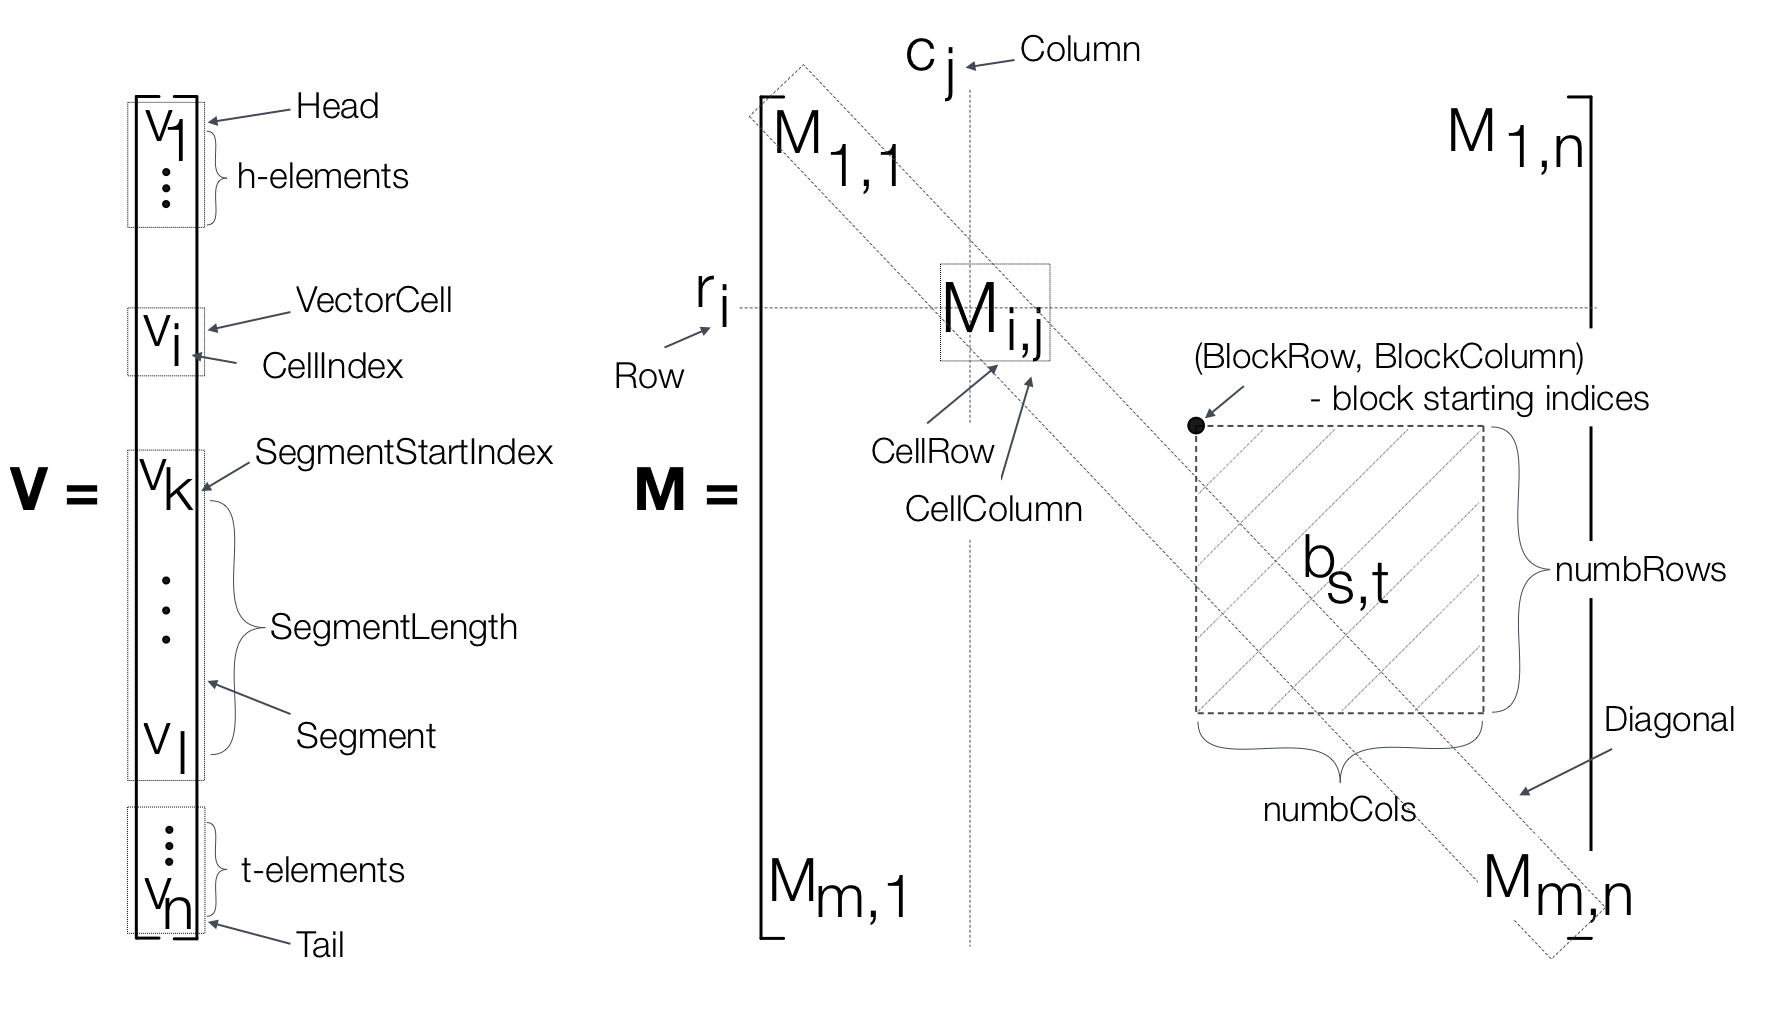
\includegraphics[width=140mm]{pics/VectorMatrixOverview.pdf}
\caption{Vector and matrix -- vocabulary and structure overview.}
\label{fig:vectorMatrix}
\end{figure}



%%%%%%%%%%%%%%%%%%%%%%%%%%%%%%%%%%%%%%%%%%%%%%%%%%%%%%%%%%%%%%%%%%%%%%
\subsection{Vector structure with examples}
\label{subsec:vectorType}
Vectors are defined to be column vectors. Row vectors can be created by taking
the transpose (with the \emph{transpose} operation still to be defined) of a column vector. 

\subsubsection{Populating vectors}
\begin{itemize}
\item
Elements
\begin{itemize}
\item
\xelem{VectorElements} is used to define all elements without indexing and takes any 
combination of the following items
\begin{itemize}
\item
\xelem{Scalar} and/or \xelem{SymbRef}
\item
\xelem{Sequence}
\end{itemize}
\item
\xelem{VectorCell} is used to define one element of the vector by specifying its index
\begin{itemize}
\item
\xelem{VectorIndex} and either
\item
\xelem{Scalar} or \xelem{SymbRef}
\end{itemize}
\item
\xelem{VectorSegment} allows to encode consecutive elements defined by the 
start/end indices by using 
\begin{itemize}
\item
\xelem{StartIndex}
\item
\xelem{SegmentLength}
\item
\xelem{VectorElements}
\end{itemize}
\end{itemize}
\item
Attributes
\begin{itemize}
\item
\xatt{default} stands for the value of not explicitly specified elements -- necessary when 
sparse vectors are encoded using \xelem{VectorCell} or \xelem{VectorSegment}
\item
\xatt{length} of the vector -- required, see \xatt{default} comments above.
\end{itemize}
\end{itemize}
Table \ref{tab:vectorsComparison} show two examples how you can encode vectors.

\begin{table}[ht!]
\setlength{\tabcolsep}{10pt}
\begin{center}
\begin{tabular}{ll}
  \hline
  \hline
 \pml version $\le$ 0.3.1 &  \pml version 0.4 \\
  \hline
% \multicolumn{2}{c}{encoding [0,2,0,0,5,0,0,0,0,0]}  \\
%  \hline
  \lstset{language=XML}
\begin{lstlisting}
<ct:Vector>
    <ct:Real>0</ct:Real>
    <ct:Real>2</ct:Real>
    <ct:Real>0</ct:Real>
    <ct:Real>0</ct:Real>
    <ct:SymbRef symbIdRef="fifthElement"/>
    <ct:Real>0</ct:Real>
    <ct:Real>0</ct:Real>
    <ct:Real>0</ct:Real>
    <ct:Real>0</ct:Real>
    <ct:Real>0</ct:Real>
</ct:Vector>
\end{lstlisting}
&
\lstset{language=XML}
\begin{lstlisting}
<ct:Vector length="10">
    <ct:VectorElements>
        <ct:Real>0</ct:Real>
        <ct:Real>2</ct:Real>
        <ct:Real>0</ct:Real>
        <ct:Real>0</ct:Real>
        <ct:SymbRef symbIdRef="fifthElement"/>
        <ct:Real>0</ct:Real>
        <ct:Real>0</ct:Real>
        <ct:Real>0</ct:Real>
        <ct:Real>0</ct:Real>
        <ct:Real>0</ct:Real>
    </ct:VectorElements>
</ct:Vector>
\end{lstlisting}  
\\
& OR
\\
--
&
\lstset{language=XML}
\begin{lstlisting}
<ct:Vector default="0" length="10">
    <ct:VectorCell>
        <ct:VectorIndex>
            <ct:Int>2</ct:Int>
        </ct:VectorIndex>
        <ct:Real>2</ct:Real>
    </ct:VectorCell>
    <ct:VectorCell>
        <ct:VectorIndex>
            <ct:Int>5</ct:Int>
        </ct:VectorIndex>
        <ct:SymbRef symbIdRef="fifthElement"/>
    </ct:VectorCell>
</ct:Vector>
\end{lstlisting} 
\\
%\hline
% \multicolumn{2}{c}{encoding [1,1,3,4,5,6,1,1,1,1]}  \\
%\hline
%-- & \lstset{language=XML}
%\begin{lstlisting}
%<ct:Vector default="1" length="10">
%    <ct:VectorSegment>
%        <ct:StartIndex>3</ct:StartIndex>
%        <ct:EndIndex>6</ct:EndIndex>
%    </ct:VectorSegment>
%</ct:Vector>
%\end{lstlisting} \\
    \hline
\end{tabular}
\caption{Comparison of vector support in the current and previous version of PharmML. In the first case a 
sparse vector [0,2,0,0,5,0,0,0,0,0] is encoded illustrating the new structure with 
\xelem{VectorElements} and \xelem{VectorCell}.  
%In the second case the vector 
%[1,1,3,4,5,6,1,1,1,1] is encoded using the \xelem{VectorSegment} element. 
In versions $\le$ 0.3.1 all vector elements had to be listed whereas the new version 
offers a \xatt{default} attribute which can be used to avoid unwanted repetitions.}
\label{tab:vectorsComparison}
\end{center}
\end{table}

\subsubsection{Reading vectors}
Once a vector is assigned, we need a mechanism for the readout of vector
elements. This is done with the \xelem{VectorSelector} element. Additionally to the 
vocabulary we used before, we have the \xelem{Head} and \xelem{Tail} methods, i.e.
two ways to extract the first or last few elements which number can be specified
explicitly. The following child elements allow flexible access to any vector element
\begin{itemize}
\item
\xelem{SymbRef} identifies the vector of interest (mandatory)
\item
\xelem{Head} allows to select any number of elements starting with the first one
\item
\xelem{Tail} allows to select any number of elements counted from the last one
\item
\xelem{Cell} is used to pick one element
\item
\xelem{Segment} allows to select a segment of a vector
\end{itemize}
For example, we would like to perform the following assignment 
\begin{align}
& m = a + V2[5] \nonumber
\end{align}
i.e. to add parameter $a$ to the fifth element of vector $V2$. 
The following code shows how this is done. 

\lstset{language=XML}
\begin{lstlisting}
            <SimpleParameter symbId="m">
                <ct:Assign>
                    <math:Equation>
                        <math:Binop op="plus">
                            <ct:SymbRef symbIdRef="a"/>
                            <ct:VectorSelector>
                                <ct:SymbRef symbIdRef="V2"/>
                                <ct:Cell>
                                    <ct:Int>5</ct:Int>
                                </ct:Cell>
                            </ct:VectorSelector>
                        </math:Binop>
                    </math:Equation>
                </ct:Assign>
            </SimpleParameter>
\end{lstlisting}
Now a more complex selection scenario using all available \xelem{VectorSelector} child 
elements: \xelem{Head}, \xelem{Index}, \xelem{Segment} and \xelem{Tail}. In this case it is 
assumed that vector V2 has 25 elements and we want to select only those specified by the
following indexes $i=1:3,\;6:8,\;11,\;18:20,\;22,\;24:25.$
\lstset{language=XML}
\begin{lstlisting}
            <SimpleParameter symbId="n">
                <ct:Assign>
                    <math:Equation>
                        <ct:VectorSelector>
                            <ct:SymbRef symbIdRef="V2"/>
                            <ct:Head><ct:Int>3</ct:Int></ct:Head>
                            <ct:Segment>
                                <ct:StartIndex><ct:Int>6</ct:Int></ct:StartIndex>
                                <ct:SegmentLength><ct:Int>3</ct:Int></ct:SegmentLength>
                            </ct:Segment>
                            <ct:Cell><ct:Int>11</ct:Int></ct:Cell>
                            <ct:Segment>
                                <ct:StartIndex><ct:Int>18</ct:Int></ct:StartIndex>
                                <ct:SegmentLength><ct:Int>3</ct:Int></ct:SegmentLength>
                            </ct:Segment>
                            <ct:Cell><ct:Int>22</ct:Int></ct:Cell>
                            <ct:Tail><ct:Int>2</ct:Int></ct:Tail>
                        </ct:VectorSelector>
                    </math:Equation>
                </ct:Assign>
            </SimpleParameter>
\end{lstlisting}


%%%%%%%%%%%%%%%%%%%%%%%%%%%%%%%%%%%%%%%%%%%%%%%%%%%%%%%%%%%%%%%%%%%%%%
\subsection{Matrix structure with examples}
\label{subsec:matrixStructure}
Similarly to the vector structure there are a few alternative options to encode a matrix.
Note, that for now matrices are allowed in the \xelem{Correlation} element only. Their use
will be extended to handle covariance matrices of multivariate distributions and objects in the 
Standardised Input/Output Model to be introduced in a future release.

\subsubsection{Populating matrices}
\begin{itemize}
\item
Elements
\begin{itemize}
\item
\xelem{MatrixRow} is used to define the matrix row-by-row using
\begin{itemize}
\item
\xelem{RowIndex} (optional) element followed by 
\item
\xelem{Scalar} and/or \xelem{SymbRef}
\item
\xelem{Sequence}
\end{itemize}
\item
\xelem{MatrixCell} is useful for matrices with few non-zero elements
\begin{itemize}
\item
mandatory elements \xelem{CellRow} and 
\item
\xelem{CellColumn} followed by
\item
\xelem{Scalar} or \xelem{SymbRef}
\end{itemize}
\item
\xelem{MatrixBlock} is useful for matrices with non-zero blocks using
\begin{itemize}
\item
\xelem{BlockStartRow} and \xelem{BlockStartColumn} followed by 
a combination of 
\item
\xelem{BlockRow} and/or \xelem{BlockCell} elements
\item
and block attributes which are identical to those of the matrix (listed below) with 
the exception of \xatt{matrixType}
\end{itemize}
\end{itemize}
\item
Attributes
\begin{itemize}
\item
\xatt{matrixType} allows to simplify the matrix encoding with following possible values
\begin{itemize}
\item
\xatt{Any} -- no requirements on the matrix.
\item
\xatt{Diagonal} -- only the diagonal values have to be specified, the rest is 
by definition zero.
\item
\xatt{LowerTriangular}/\xatt{UpperTriangular} -- only diagonal and off-diagonal
matrix elements below or above the diagonal are non-zero and have to be 
specified, respectively.
\item
\xatt{Symmetric} -- due to symmetry only the off-diagonal matrix elements 
below or above the diagonal have to be specified.
\end{itemize}
\item
\xatt{numbCols, numbRows} matrix dimensions -- required for sparse matrices, see 
default attributes comments below.
\item
\xatt{diagDefault} the default value on the diagonal -- required when 
sparse matrices are encoded using \xelem{MatrixCell} or \xelem{MatrixBlock}
\item
\xatt{offDiagDefault}  the default off-diagonals value -- see comments above
\item
\xatt{symbId} -- (optional) identifier for the matrix.
\end{itemize}


\end{itemize}
If \xelem{MatrixCell} is used the attributes \xatt{matrixType}, \xatt{diagDefault} and 
\xatt{offDiagDefault} can or have to used, dependent on the matrix content. These two 
options are demonstrated with the following matrix, $\Sigma$,
\label{subsec:matrixType}
\begin{align}
\Sigma = 
  \begin{bmatrix} 
  1 & \Sigma_{12} & 0 & 0 \\
  0 & 1 & \Sigma_{23} & 0 \\
  \Sigma_{31} & 0 & 1 & 0 \\
  0 & 0 & 0 & \Sigma_{44} \end{bmatrix} 
\end{align}

\subsubsection{Implementation of $\Sigma$ as full matrix}
This is a straightforward implementation of every matrix element explicitly using
the \xelem{MatrixRow} elements.  

  \lstset{language=XML}
\begin{lstlisting}
                <!-- omitted <Correlation> tag -->
                <ct:Assign>
                    <ct:Matrix symbId="Sigma" matrixType="Any">
                        <ct:MatrixRow>
                            <ct:RowIndex><ct:Int>1</ct:Int></ct:RowIndex>
                            <ct:Real>1</ct:Real>
                            <ct:SymbRef symbIdRef="Sigma12"/>
                            <ct:Real>0</ct:Real>
                            <ct:Real>0</ct:Real>
                        </ct:MatrixRow>
                        <ct:MatrixRow>
                            <ct:RowIndex><ct:Int>2</ct:Int></ct:RowIndex>
                            <ct:Real>0</ct:Real>
                            <ct:Real>1</ct:Real>
                            <ct:SymbRef symbIdRef="Sigma23"/>
                            <ct:Real>0</ct:Real>
                        </ct:MatrixRow>
                        <ct:MatrixRow>
                            <ct:RowIndex><ct:Int>3</ct:Int></ct:RowIndex>
                            <ct:SymbRef symbIdRef="Sigma31"/>
                            <ct:Real>0</ct:Real>
                            <ct:Real>1</ct:Real>
                            <ct:Real>0</ct:Real>
                        </ct:MatrixRow>
                        <ct:MatrixRow>
                            <ct:RowIndex><ct:Int>4</ct:Int></ct:RowIndex>
                            <ct:Real>0</ct:Real>
                            <ct:Real>0</ct:Real>
                            <ct:Real>0</ct:Real>
                            <ct:SymbRef symbIdRef="Sigma44"/>
                        </ct:MatrixRow>
                    </ct:Matrix>
                </ct:Assign>
\end{lstlisting}
 
\subsubsection{Implementation of $\Sigma$ as sparse matrix}
Here the $\Sigma$ matrix is implemented using \xelem{MatrixCell} elements.
More specifically only four values have to be stored. The test is encoded using 
\xatt{diagDefault} and \xatt{offDiagDefault} attributes.

\lstset{language=XML}
\begin{lstlisting}
                <!-- omitted <Correlation> block -->
                <ct:Assign>
                    <ct:Matrix symbId="Sigma" matrixType="Any" diagDefault="1" offDiagDefault="0">
                        <ct:MatrixCell>
                            <ct:CellRow><ct:Int>1</ct:Int></ct:CellRow>
                            <ct:CellColumn><ct:Int>2</ct:Int></ct:CellColumn>
                            <ct:SymbRef symbIdRef="Sigma12"/>
                        </ct:MatrixCell>
                        <ct:MatrixCell>
                            <ct:CellRow><ct:Int>2</ct:Int></ct:CellRow>
                            <ct:CellColumn><ct:Int>3</ct:Int></ct:CellColumn>
                            <ct:SymbRef symbIdRef="Sigma23"/>
                        </ct:MatrixCell>
                        <ct:MatrixCell>
                            <ct:CellRow><ct:Int>3</ct:Int></ct:CellRow>
                            <ct:CellColumn><ct:Int>1</ct:Int></ct:CellColumn>
                            <ct:SymbRef symbIdRef="Sigma31"/>
                        </ct:MatrixCell>
                        <ct:MatrixCell>
                            <ct:CellRow><ct:Int>4</ct:Int></ct:CellRow>
                            <ct:CellColumn><ct:Int>4</ct:Int></ct:CellColumn>
                            <ct:SymbRef symbIdRef="Sigma44"/>
                        </ct:MatrixCell>
                    </ct:Matrix>
                </ct:Assign>
\end{lstlisting}  
Note the use of the attributes \xatt{diagDefault} and \xatt{offDiagDefault}
set with either 1 or 0, respectively, which makes the matrix encoding 
very efficient.

\subsubsection{Example 2 -- \emph{face} matrix}
Figure \ref{fig:faceMatrix} shows how a sparse matrix can be encoded in an
efficient way using a combination of
\begin{itemize}
\item
\xelem{MatrixBlock}
\item
\xelem{MatrixCell} and
\item
\xelem{MatrixRow}.
\end{itemize}
More specifically, the use of two 2x2-blocks, three cells and one matrix row 
is sufficient to encode the hypothetical \emph{face} matrix because the rest 
can be handled with attributes. Figure \ref{fig:faceMatrix} and the code
next to it shows how the elements are defined. Attributes \xatt{diagDefault} 
and \xatt{offDiagDefault} are both set to 1.
Note that the \xelem{RowIndex} of the block's rows are specified relative to 
the block start coordinates, \xelem{BlockStartRow} and \xelem{BlockStartColumn}.
Consequently, the first block row consisting of two 'X' symbols has the index 1, 
the second has the index 2. In contrast the last row is defined using \xelem{RowIndex} 
relative to the main matrix. The attributes \xatt{numbRows} and \xatt{numbCols} 
of the matrix are required due to its sparse nature.


\begin{figure}
\centering
\begin{minipage}[c]{.48\textwidth}
\centering
 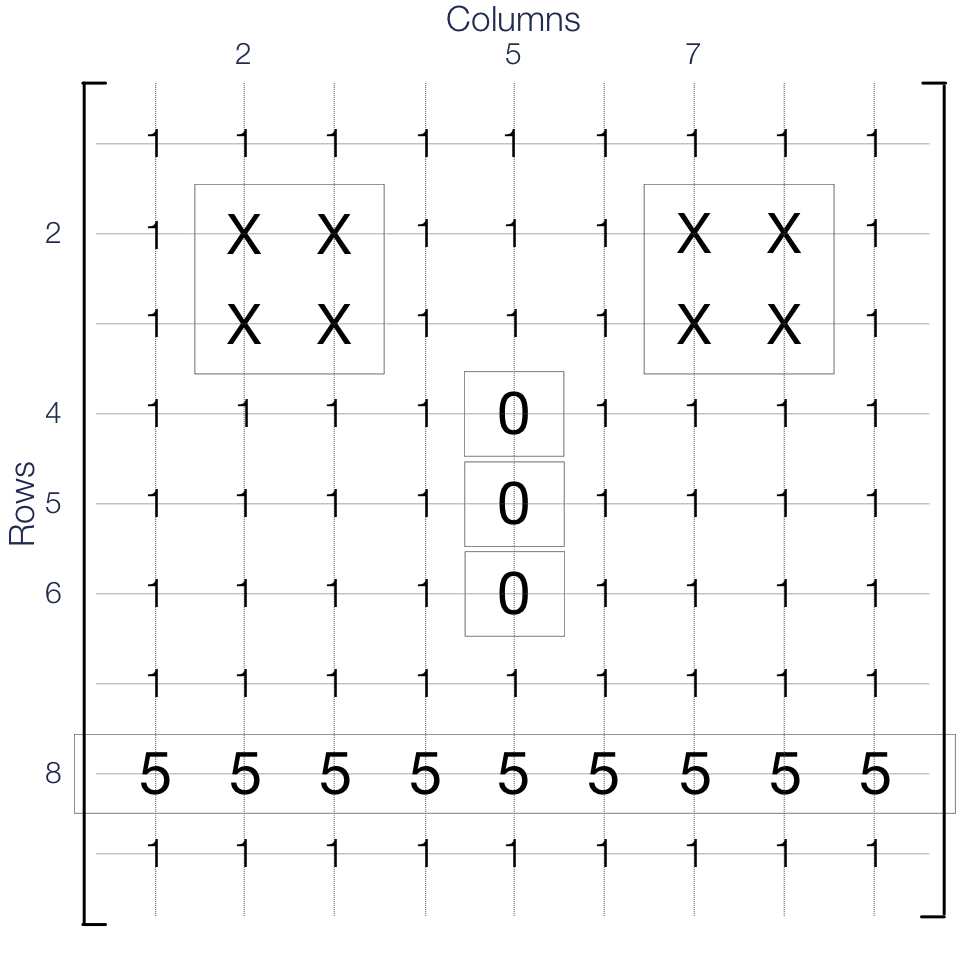
\includegraphics[width=75mm]{pics/faceMatrix.jpg}
\caption{Matrix example consisting of two blocks, three cells and one row.
They contain either numerical values or variables names. All other elements 
are defined but the attributes \xatt{diagDefault} and \xatt{offDiagDefault}, 
here both set to 1. \xelem{RowIndex} of the blocks are specified relative to 
the block start coordinates while the indexes of the cells and full matrix rows 
are absolute. The attributes \xatt{numbRows} and \xatt{numbCols} of the
matrix are required due to its sparse nature.}
\label{fig:faceMatrix}
\end{minipage}
\begin{minipage}[c]{.44\textwidth}
\lstset{language=XML}
\begin{lstlisting}
<Correlation deviationMatrixType="CovMatrix">
    <ct:VariabilityReference>
        <ct:SymbRef symbIdRef="subject"/>
    </ct:VariabilityReference>
    <Matrix symbId="faceMatrix" matrixType="Any" 
    	diagDefault="1" offDiagDefault="1">
        <!-- Left eye block -->
        <ct:MatrixBlock>
            <ct:BlockStartRow>
                <ct:Int>2</ct:Int>
            </ct:BlockStartRow>
            <ct:BlockStartColumn>
                <ct:Int>2</ct:Int>
            </ct:BlockStartColumn>
            <ct:BlockRow>
                <ct:RowIndex>
                  <ct:Int>1</ct:Int>
                </ct:RowIndex>
                <ct:SymbRef symbIdRef="X"/>
                <ct:SymbRef symbIdRef="X"/>
            </ct:BlockRow>
            <ct:BlockRow>
                <ct:RowIndex>
                   <ct:Int>2</ct:Int>
                </ct:RowIndex>
                <ct:SymbRef symbIdRef="X"/>
                <ct:SymbRef symbIdRef="X"/>
            </ct:BlockRow>
        </ct:MatrixBlock>
        <!-- Right eye block -->
        <ct:MatrixBlock>
            <ct:BlockStartRow>
                <ct:Int>2</ct:Int>
            </ct:BlockStartRow>
            <ct:BlockStartColumn>
                <ct:Int>7</ct:Int>
            </ct:BlockStartColumn>
            <!-- omitted - identical to left block -->
        </ct:MatrixBlock>
        <!-- Nose blocks -->
        <ct:MatrixCell>
            <ct:CellRow>
                <ct:Int>5</ct:Int>
            </ct:CellRow>
            <ct:CellColumn>
                <ct:Int>5</ct:Int>
            </ct:CellColumn>
            <ct:Real>0</ct:Real>
        </ct:MatrixCell>
        <!-- omitted middle cell -->
        <ct:MatrixCell>
            <ct:CellRow>
                <ct:Int>7</ct:Int>
            </ct:CellRow>
            <ct:CellColumn>
                <ct:Int>5</ct:Int>
            </ct:CellColumn>
            <ct:Real>0</ct:Real>
        </ct:MatrixCell>
        <!-- Mouth row -->
        <ct:MatrixRow default="8">
            <ct:RowIndex>
           <ct:SymbRef symbIdRef="W"/>
            </ct:RowIndex>
        </ct:MatrixRow>
    </Matrix>
</Correlation>
\end{lstlisting}
\end{minipage}
\end{figure}





%\subsubsection{Example 3 -- Lower/upper triangular matrix}
%...to be finished
%

\subsubsection{Example 3 -- Block-diagonal matrix}
A typical matrix application example is the specification of the
correlation matrix of the random effects, see a screenshot for the 
Monolix GUI, Figure \ref{fig:corrMatrixMonolix}, \cite{MLXTRAN4.3.2Specification:2014}. 
This is another example of a sparse matrix with the blocks as the only non-zero 
elements of the matrix. Using attributes \xatt{diagDefault} and \xatt{offDiagDefault} 
makes the encoding an easy task leaving only the blocks to be defined explicitly. 

\begin{figure}[htb!]
\centering
  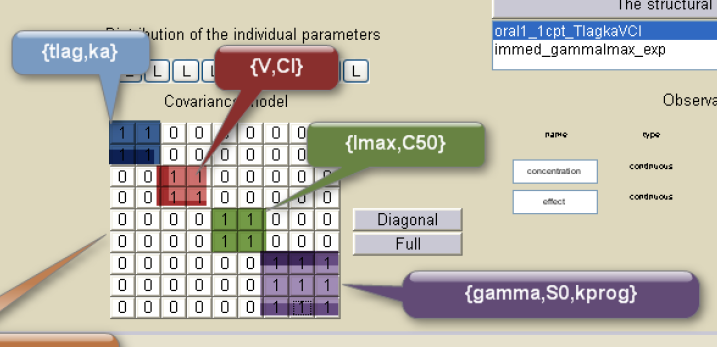
\includegraphics[width=90mm]{pics/corrMatrixMonolix}
 \caption{Correlation matrix encoded using the Monolix GUI, \cite{MLXTRAN4.3.2Specification:2014}.}
 \label{fig:corrMatrixMonolix}
\end{figure}

\lstset{language=XML}
\begin{lstlisting}
<Correlation deviationMatrixType="CorrMatrix">
    <ct:VariabilityReference>
        <ct:SymbRef symbIdRef="subject"/>
    </ct:VariabilityReference>
    <Matrix symbId="Omega" matrixType="Any" diagDefault="1" offDiagDefault="0">
        <!-- tlag, ka - block -->
        <ct:MatrixBlock>
            <ct:BlockStartRow><ct:Int>1</ct:Int></ct:BlockStartRow>
            <ct:BlockStartColumn><ct:Int>1</ct:Int></ct:BlockStartColumn>
            <ct:BlockRow>
                <ct:RowIndex><ct:Int>1</ct:Int></ct:RowIndex>
                <ct:Int>1</ct:Int><ct:Int>1</ct:Int>
            </ct:BlockRow>
            <ct:BlockRow>
                <ct:RowIndex><ct:Int>2</ct:Int></ct:RowIndex>
                <ct:Int>1</ct:Int><ct:Int>1</ct:Int>
            </ct:BlockRow>
        </ct:MatrixBlock>
        <!-- V, CL - block -->
        <ct:MatrixBlock>
            <ct:BlockStartRow><ct:Int>3</ct:Int></ct:BlockStartRow>
            <ct:BlockStartColumn><ct:Int>3</ct:Int></ct:BlockStartColumn>
            <ct:BlockRow>
                <ct:RowIndex><ct:Int>1</ct:Int></ct:RowIndex>
                <ct:Int>1</ct:Int><ct:Int>1</ct:Int>
            </ct:BlockRow>
            <ct:BlockRow>
                <ct:RowIndex><ct:Int>2</ct:Int></ct:RowIndex>
                <ct:Int>1</ct:Int><ct:Int>1</ct:Int>
            </ct:BlockRow>
        </ct:MatrixBlock>
        <!-- Imax, C50 - block -->
        <ct:MatrixBlock>
            <ct:BlockStartRow><ct:Int>5</ct:Int></ct:BlockStartRow>
            <ct:BlockStartColumn><ct:Int>5</ct:Int></ct:BlockStartColumn>
            <ct:BlockRow>
                <ct:RowIndex><ct:Int>1</ct:Int></ct:RowIndex>
                <ct:Int>1</ct:Int><ct:Int>1</ct:Int>
            </ct:BlockRow>
            <ct:BlockRow>
                <ct:RowIndex><ct:Int>2</ct:Int></ct:RowIndex>
                <ct:Int>1</ct:Int><ct:Int>1</ct:Int>
            </ct:BlockRow>
        </ct:MatrixBlock>
        <!-- gammma, S0, kprog - block -->
        <ct:MatrixBlock>
            <ct:BlockStartRow><ct:Int>7</ct:Int></ct:BlockStartRow>
            <ct:BlockStartColumn><ct:Int>7</ct:Int></ct:BlockStartColumn>
            <ct:BlockRow>
                <ct:RowIndex><ct:Int>1</ct:Int></ct:RowIndex>
                <ct:Int>1</ct:Int><ct:Int>1</ct:Int><ct:Int>1</ct:Int>
            </ct:BlockRow>
            <ct:BlockRow>
                <ct:RowIndex><ct:Int>2</ct:Int></ct:RowIndex>
                <ct:Int>1</ct:Int><ct:Int>1</ct:Int><ct:Int>1</ct:Int>
            </ct:BlockRow>
            <ct:BlockRow>
                <ct:RowIndex><ct:Int>3</ct:Int></ct:RowIndex>
                <ct:Int>1</ct:Int><ct:Int>1</ct:Int><ct:Int>1</ct:Int>
            </ct:BlockRow>
        </ct:MatrixBlock>
    </Matrix>
</Correlation>
\end{lstlisting}

%%%%%%%%%%%%%%%%%%%%%%%%%%%%%%%%%%%%%%%%%%%%%%%%%%
\subsubsection{Reading matrices and their subelements.}
Following code shows few examples of how to access 
\begin{itemize}
\item
single element
\item
single row or
\item
\{flag,ka\} block
\end{itemize}
from the $\Omega$ matrix defined in previous example, see Figure \ref{fig:corrMatrixMonolix}.

\lstset{language=XML}
\begin{lstlisting}
            <!-- extract one element -->
            <SimpleParameter symbId="rho_tlag_ka">
                <ct:Assign>
                    <math:Equation>
                        <ct:MatrixSelector>
                            <ct:SymbRef symbIdRef="Omega"/>
                            <ct:Cell>
                                <ct:RowIndex><ct:Int>1</ct:Int></ct:RowIndex>
                                <ct:ColumnIndex><ct:Int>2</ct:Int></ct:ColumnIndex>
                            </ct:Cell>
                        </ct:MatrixSelector>
                    </math:Equation>
                </ct:Assign>
            </SimpleParameter>
            
            <!-- extract 2nd row -->
            <ct:Variable symbolType="real" symbId="SecondRow">
                <ct:Assign>
                    <math:Equation>
                        <ct:MatrixSelector>
                            <ct:SymbRef symbIdRef="Omega"/>
                            <ct:Row>
                                <ct:Int>2</ct:Int>
                            </ct:Row>
                        </ct:MatrixSelector>
                    </math:Equation>
                </ct:Assign>
            </ct:Variable>
            
            <!-- extract {tlag,ka} block -->
            <ct:Variable symbolType="real" symbId="Rho_tlag_ka">
                <ct:Assign>
                    <math:Equation>
                        <ct:MatrixSelector>
                            <ct:SymbRef symbIdRef="Omega"/>
                            <ct:Block>
                                <ct:BlockStartRow><ct:Int>1</ct:Int></ct:BlockStartRow>
                                <ct:BlockStartColumn><ct:Int>1</ct:Int></ct:BlockStartColumn>
                                <ct:RowsNumber><ct:Int>2</ct:Int></ct:RowsNumber>
                                <ct:ColumnsNumber><ct:Int>2</ct:Int></ct:ColumnsNumber>
                            </ct:Block>
                        </ct:MatrixSelector>
                    </math:Equation>
                </ct:Assign>
            </ct:Variable>
\end{lstlisting}


\subsection{Typing rules}
-- Subscripting has the highest precedence compared to any other arithmetic operation.


%%%%%%%%%%%%%%%%%%%%%%%%%%%%%%%%%%%%%%%%%%%%%%%%%%
%%%%%%%%%%%%%%%%%%%%%%%%%%%%%%%%%%%%%%%%%%%%%%%%%%
\section{Other changes}
\label{sec:otherChanges}
\subsection{Sum and products using indexes}
Sum and product symbols are frequently used in various model formulations, see for 
example section \ref{subsec:categoricalData}. Both have avery similar structure and 
consist of following elements
\begin{itemize}
\item
\xelem{SymbRef} -- to define the variable for which the sum or product is defined. 
\item
\xelem{SumIndex} or \xelem{ProductIndex} -- (optional) identifies the index.
\item
\xelem{LowLimit} and \xelem{UpLimit} -- need to restrict the value of the index.
\end{itemize}
Table \ref{tab:sumAndProduct} contains two basic examples of the use of sum and
product.

\begin{table}[ht!]
\setlength{\tabcolsep}{15pt}
\begin{center}
\begin{tabular}{ll}
  \hline
  \hline
 Expression &  \pml version 0.4 implementation\\
  \hline
 \multicolumn{2}{c}{Product}  \\
  \hline
$W = \prod_{i=1}^{N} V_i $
&
\lstset{language=XML}
\begin{lstlisting}
            <SimpleParameter symbId="W">
                <ct:Assign>
                    <math:Equation>
                        <ct:Product>
                            <ct:SymbRef symbIdRef="V"/>
                            <ct:ProductIndex>
                                <ct:SymbRef symbIdRef="i"/>
                            </ct:ProductIndex>
                            <ct:LowLimit>
                                <ct:Int>1</ct:Int>
                            </ct:LowLimit>
                            <ct:UpLimit>
                                <ct:SymbRef symbIdRef="N"/>
                            </ct:UpLimit>
                        </ct:Product>
                    </math:Equation>
                </ct:Assign>
            </SimpleParameter>
\end{lstlisting}
\\
  \hline
 \multicolumn{2}{c}{Sum}  \\
  \hline
$M = \sum_{i=1}^{N} V_i $
&
\lstset{language=XML}
\begin{lstlisting}
            <SimpleParameter symbId="M">
                <ct:Assign>
                    <math:Equation>
                        <ct:Sum>
                            <ct:SymbRef symbIdRef="V"/>
                            <ct:SumIndex>
                                <ct:SymbRef symbIdRef="i"/>
                            </ct:SumIndex>
                            <ct:LowLimit>
                                <ct:Int>1</ct:Int>
                            </ct:LowLimit>
                            <ct:UpLimit>
                                <ct:SymbRef symbIdRef="N"/>
                            </ct:UpLimit>
                        </ct:Sum>
                    </math:Equation>
                </ct:Assign>
            </SimpleParameter>
\end{lstlisting}
\\
    \hline
\end{tabular}
\caption{Implementation examples for sigma sum element, $\sum$, and product, $\prod$.}
\label{tab:sumAndProduct}
\end{center}
\end{table}


%%%%%%%%%%%%%%%%%%%%%%%%%%%%%%%%%%%%%%%%%%%%%%%%%%
\subsection{Correlation matrix update}
\label{sec:correlationMatrix}
Changes in the matrix were necessary to arrive at a consistent, generic matrix definition.
Previous format and use was determined by the correlation/covariance structure 
requirements only and was too limiting for general use. As explained in section 
\ref{sec:vectorsAndMatrices}, \xatt{matrixType} has been renamed in \xatt{deviationMatrixType}
and relocated to the \xelem{Correlation} element. The original \xatt{matrixType} 
is now populated with the names of general matrix formats. The attribute 
\xatt{deviationMatrixType} is optional and should only be used in connection with matrices.
See Figure \ref{tab:newMatrixStructure} for a comparison of the current and previous deviance 
matrix structure.

\begin{table}[ht!]
\setlength{\tabcolsep}{5pt}
\begin{center}
\begin{tabular}{ll}
  \hline
Definition in $\leq$ 0.3.1 versions 	& Definition in 0.4 version  \\
  \hline
%			\multicolumn{2}{c}{Mapping in a \xelem{CategoricalData} model}  \\  [.5ex]
  \hline
\lstset{language=XML}
\begin{lstlisting}
<Correlation>
    <ct:VariabilityReference>
        <ct:SymbRef symbIdRef="iiv"/>
    </ct:VariabilityReference>
    <Matrix matrixType="CorrMatrix">
        <ct:MatrixRow>
            <ct:Real>1</ct:Real>
            <ct:Real>2</ct:Real>
        </ct:MatrixRow>
        <ct:MatrixRow>
            <ct:Real>3</ct:Real>
            <ct:Real>4</ct:Real>
        </ct:MatrixRow>
    </Matrix>
</Correlation>
\end{lstlisting}
&
\lstset{language=XML}
\begin{lstlisting}
<Correlation deviationMatrixType="CorrMatrix">
    <ct:VariabilityReference>
        <ct:SymbRef symbIdRef="iiv"/>
    </ct:VariabilityReference>
    <Matrix matrixType="Any">
        <ct:MatrixRow>
            <ct:Real>1</ct:Real>
            <ct:Real>2</ct:Real>
        </ct:MatrixRow>
        <ct:MatrixRow>
            <ct:Real>3</ct:Real>
            <ct:Real>4</ct:Real>
        </ct:MatrixRow>
    </Matrix>
</Correlation>
\end{lstlisting}
\\
    \hline
\end{tabular}
\caption{Changes in the matrix structure. The new attribute \xatt{deviationMatrixTyp} carries 
now values which were stored by \xatt{matrixType} in previous version, i.e. \{\xatt{CorrMatrix}, 
\xatt{CovMatrix}, \xatt{StDevCorrMatrix}, \xatt{Cholesky}\}. The attribute \xatt{matrixType} is 
now having the general values characterising a matrix, such as: \{\xatt{Any}, \xatt{LowerTriangular}, 
\xatt{UpperTriangular}, \xatt{Diagonal}, \xatt{Symmetric}\}.}
\label{tab:newMatrixStructure}
\end{center}
\end{table}


%%%%%%%%%%%%%%%%%%%%%%%%%%%%%%%%%%%%%%%%%%%%%%%%%%
\subsection{Categorical data/covariates mapping  {\color{red} \scshape{*table updated}}}
\label{subsec:catDataCovariatesMapping}

As indicated already in section \ref{sec:catDataMapping} the mapping of categories symbols 
as stored in the data set and used in the model is now done in the \xelem{ModellingSteps} 
part of PharmML. The \xelem{CategoryMapping} element is used with attributes
\begin{itemize}
\item
\xatt{dataSymbol} -- the symbol as used the external dataset, e.g. 0/1 for 'SEX' covariates
or \{1,2,3\} for categories of a categorical data model.
\item
\xatt{modelSymbol} -- the symbol as used the model, e.g. F/M for SEX covariates
or \{cat1, cat2, cat3\} for categories of a categorical data model
\end{itemize}
see Table \ref{tab:categoryMapping} for examples.

\begin{table}[ht!]
\setlength{\tabcolsep}{1pt}
\begin{center}
\begin{tabular}{ll}
  \hline
Definition of categories  	& \xelem{CategoryMapping} in \xelem{ColumnMapping} \\
  \hline
\multicolumn{2}{c}{Mapping of discrete data categories \xelem{CategoricalData} model}  \\  [.5ex]
  \hline
\lstset{language=XML}
\begin{lstlisting}
<ObservationModel blkId="om1">
    <CategoricalData ordered="yes">
        <ListOfCategories> 
            <Category symbId="cat1"/>
            <Category symbId="cat2"/>
            <Category symbId="cat3"/>
        </ListOfCategories>
        
        <CategoryVariable symbId="Y"/>
        <!-- omitted the rest -->
\end{lstlisting}
&
\lstset{language=XML}
\begin{lstlisting}
<ColumnMapping>
    <ColumnRef columnIdRef="DV"/>
    <ct:SymbRef blkIdRef="om1" symbIdRef="Y"/>
    <CategoryMapping>
        <Map dataSymbol="1" modelSymbol="cat1"/>
        <Map dataSymbol="2" modelSymbol="cat2"/>
        <Map dataSymbol="3" modelSymbol="cat3"/>
    </CategoryMapping>
</ColumnMapping>

\end{lstlisting}
\\
    \hline
			\multicolumn{2}{c}{Mapping of categories of discrete covariates in \xelem{CovariateModel}}  \\  [.5ex]
  \hline
\lstset{language=XML}
\begin{lstlisting}
<CovariateModel blkId="cm1">
    <Covariate symbId="SEX">
        <Categorical>
          <Category catId="F">
              <Probability>
                  <ct:Real>.55</ct:Real>
              </Probability>
          </Category>                    
          <Category catId="M">
              <Probability>
                  <ct:Real>.45</ct:Real>
              </Probability>
          </Category>
        </Categorical>
    </Covariate>
</CovariateModel>
\end{lstlisting}
&
\lstset{language=XML}
\begin{lstlisting}
<ColumnMapping>
    <ColumnRef columnIdRef="COV"/>
    <ct:SymbRef blkIdRef="cm1" symbIdRef="SEX"/>
    <CategoryMapping>
        <Map dataSymbol="1" modelSymbol="F"/>
        <Map dataSymbol="0" modelSymbol="M"/>
    </CategoryMapping>
</ColumnMapping>
\end{lstlisting}
\\
    \hline
\end{tabular}
\caption{Examples of category mapping for (top) discrete data categories in the categorical data model. 
(Bottom) mapping of categories of discrete covariates in \xelem{CovariateModel}.}
\label{tab:categoryMapping}
\end{center}
\end{table}


%%%%%%%%%%%%%%%%%%%%%%%%%%%%%%%%%%%%%%%%%%%%%%%%%%%
%\subsubsection{Mapping for categorical data}
%\subsubsection{Mapping for categorical covariates}

%\subsubsection{LhsTransformationType and LRhsTransformationType}
%does it matter for the users?
%- BothSideTransformation
%for 
%1. parameter model of type GaussianModel
%2. observation error of type \xelem{Standard} -  GaussianObsError 

%%%%%%%%%%%%%%%%%%%%%%%%%%%%%%%%%%%%%%%%%%%%%%%%%%
\subsection{Logarithm notation -- unified}
Previously, two symbols existed to express the natural logarithm, $\log$ and $\ln$. 
To avoid confusions, the $ln$ symbol has been removed. The following logarithm related functions
are now available
\begin{itemize}
\item
$\log$ -- the natural logarithm
\item
$\log$2 - the base-2 (binary) logarithm 
\item
$\log$10 - the base-10 (decadic) logarithm
\end{itemize}

%%%%%%%%%%%%%%%%%%%%%%%%%%%%%%%%%%%%%%%%%%%%%%%%%%
\subsection{Metadata \xatt{id}}
... is now available for every element of the schema. This allows to annotate virtually any 
element of a model.

%%%%%%%%%%%%%%%%%%%%%%%%%%%%%%%%%%%%%%%%%%%%%%%%%%
\subsection{New attribute \xatt{implementedBy} in the root element}
The new attribute \xatt{implementedBy} is helpful to keep track on the authorship of 
a PharmML encoded file. 


\lstset{language=XML}
\begin{lstlisting}
<PharmML xmlns="http://www.pharmml.org/2013/03/PharmML"
    xmlns:xsi="http://www.w3.org/2001/XMLSchema-instance"
    ...
    writtenVersion="0.4" implementedBy="JamesBond" id="i1">
    
    <ct:Name>Testing new attribute</ct:Name>
    ...
\end{lstlisting}


%%%%%%%%%%%%%%%%%%%%%%%%%%%%%%%%%%%%%%%%%%%%%%%%%%
%%%%%%%%%%%%%%%%%%%%%%%%%%%%%%%%%%%%%%%%%%%%%%%%%%
%%%%%%%%%%%%%%%%%%%%%%%%%%%%%%%%%%%%%%%%%%%%%%%%%%
\chapter{Changes in 0.4.1}


%%%%%%%%%%%%%%%%%%%%%%%%%%%%%%%%%%%%%%%%%%%%%%%%%%
\section{Other changes}
\label{sec:otherChanges2}
\subsection{Additional link function}

\begin{itemize}
\item
$\rm loglog$ -- the log-log function
\begin{align}
& f(\mu) = \log(-\log(\mu)) \nonumber
\end{align}
\item
$\rm comloglog$ -- the complementary log-log function
\begin{align}
& f(\mu) = \log(-\log(1-\mu)) \nonumber
\end{align}
\end{itemize}

\subsection{Extensions in vector/matrix indexing definition}

Although all of the listed complex models were encodable in PharmML,
the implementation was hampered by the missing expression assignments to 
indexes and sum/product arguments -- this is fixed now as the following table shows

\begin{table}[ht!]
\setlength{\tabcolsep}{5pt}
\begin{center}
\begin{tabular}{ll}
  \hline
Definition in $\leq$ 0.3.1 versions 	& Definition in 0.4 version  \\
  \hline
%			\multicolumn{2}{c}{Mapping in a \xelem{CategoricalData} model}  \\  [.5ex]
  \hline
\lstset{language=XML}
\begin{lstlisting}
<Sum>

</Sum>
\end{lstlisting}
&
\lstset{language=XML}
\begin{lstlisting}
<Sum>

</Sum>
\end{lstlisting}
\\
    \hline
\end{tabular}
\caption{Improved index and sum/product expressions.}
\label{tab:fixedIndexExpressions}
\end{center}
\end{table}

\subsection{Examples for sum application}

\subsubsection{Sum in PD models}

\begin{figure}[htb!]
\centering
  \includegraphics[width=50mm,angle=-90]{pics/PDWithSumModel.jpg}
 \caption{}
 \label{fig:myplot}
\end{figure}

\subsubsection{Sum in categorical data models}

\begin{figure}[htb!]
\centering
  \includegraphics[width=60mm,angle=-90]{pics/CategoricalWithSumModel.jpg}
 \caption{}
 \label{fig:myplot}
\end{figure}

\subsection{Discrete data -- missing element in sim steps added}
Note - new element \\
discrete can be defined 
\begin{table}[ht!]
\setlength{\tabcolsep}{5pt}
\begin{center}
\begin{tabular}{ll}
  \hline
Definition in $\leq$ 0.3.1 versions 	& Definition in 0.4 version  \\
  \hline
%			\multicolumn{2}{c}{Mapping in a \xelem{CategoricalData} model}  \\  [.5ex]
  \hline
\lstset{language=XML}
\begin{lstlisting}
<Sum>

</Sum>
\end{lstlisting}
&
\lstset{language=XML}
\begin{lstlisting}
<Sum>

</Sum>
\end{lstlisting}
\\
    \hline
\end{tabular}
\caption{Discrete observations possible with continuous once}
\label{tab:fixedIndexExpressions}
\end{center}
\end{table}

\subsection{Vector element names changed}

VectorIndex $-->$ CellIndex \\
SegmentIndex $-->$ SegmentStartIndex \\


%%%%%%%%%%%%%%%%%%%%%%%%%%%%%%%%%%%%%%%%%%%%%%%%%%
%%%%%%%%%%%%%%%%%%%%%%%%%%%%%%%%%%%%%%%%%%%%%%%%%%
%%%%%%%%%%%%%%%%%%%%%%%%%%%%%%%%%%%%%%%%%%%%%%%%%%
\appendix

\chapter{Code examples}
\label{chapter:codeExamples}
 
% INPUT
%%%%%%%%%%%%%%%%%%%%%%%%%%%%%%%%%%%%%%%%%%%%%%%%%%%%%%%%%%%%%%%%
%%%%%%%%%%%%%%%%%%%%%%%%%%%%%%%%%%%%%%%%%%%%%%%%%%%%%%%%%%%%%%%%
\section{Count data models}
\label{sec:countDataModels}


%%%%%%%%%%%%%%%%%%%%%%%%%%%%%%%%%%%%%%%%%%%%%%%%%%%%%%%%%%%%%%%%
\subsection{Homogenous Poisson model -- PM}
\label{subsec:PMmodel}

\paragraph{Observation model}

\begin{itemize}
\item
Type of observed variable -- discrete/count
\item
Model name: Homogenous Poisson process
\item
Count variable: $y$
\item
Probability mass function (PMF)
\begin{eqnarray}
&& P(y=k; \lambda) = \frac{\lambda^k \exp(-\lambda)}{k!} \nonumber
\end{eqnarray}
\item
Link function: $\log$
\item
Constant rate parameter $\lambda$ -- \emph{homogenous Poisson process}:
\begin{eqnarray}
&& \lambda(t_{ij}, \psi_{ij}) = \lambda_{i} \nonumber
\end{eqnarray}
\end{itemize}


\paragraph{Individual parameter model}
\begin{eqnarray}
\lambda & \sim& \mbox{logNormal}(\lambda_{\rm pop}, \omega_{\lambda});  \quad \lambda_{\rm pop}=1,\quad \omega_{\lambda}=0.6 \nonumber
\end{eqnarray}


%\begin{center}
%\begin{longtable}{lll}
%\hline
%\hline
%\pml element 			&  version $\le$ 0.3.1 					& version 0.4 \\
%or modelling aspect 		&								& \\
%\hline
%Delay differential equations (DDE) 	& \emph{not supported}		& \xelem{Delay} and \xelem{History}  \\
%(see \textsection\ref{sec:DDmodels})	& 					& the latter with child elements \\ 
%						&							& -- \xelem{HistoryValue} and \\
%						&							& -- \xelem{HistoryTime} {\color{red} \scshape{new}} \\ 
%\hline
%Extended matrix and vector support & supported but			&  ... \\
%						& without indexing 				& \\
%\hline
%%row1						&  ... \\
%\hline
%\caption{Overview of major differences between versions 0.4 and 0.3.1}
%\label{figTable:overviewTable}
%\end{longtable}
%\end{center}


%\begin{center}
%\begin{longtable}{lll}
%\hline
%\end{longtable}
%\end{center}

\subsubsection{NM-TRAN code:}
Code provided by Elodie Plan.

\myStartLine

%\lstset{language=MLXTRANcode}
\lstset{language=NONMEMdataSet}
\begin{lstlisting}
$PROB Poisson distribution function 
$DATA data.csv IGNORE=@ 
$INPUT ID TIME DV

$PRED 
; Parameters
 LAMB=THETA(1)*EXP(ETA(1))

; Factorial approximation 
 IF(DV.LE.1) THEN
     LFAC=0 
     ELSE 
     LFAC = DV*LOG(DV)-DV + LOG(DV*(1+4*DV*(1+2*DV)))/6 +LOG(3.1415)/2
 ENDIF

; Likelihood definition  
 LPOIS = -LAMB+DV*LOG(LAMB)-LFAC 
 Y = -2*LPOIS

; Simulation code 
 IF (ICALL.EQ.4) THEN
     LAMB=THETA(1)*EXP(ETA(1)) 
     T=0 
     N=0 
     DO WHILE (T.LT.1)
          CALL RANDOM (2,R) 
          T=T-LOG(1-R)/LAMB 
          IF (T.LT.1) N=N+1
     END DO
     DV=N 
ENDIF

$THETA (0,0.5)             ; LAMBDA

$OMEGA 0.1

$ESTIMATION MAXEVAL=9999 METHOD=COND LAPLACE -2LL 
$COV 
;$SIMULATION (361734) (474980 UNIFORM) ONLYSIM NOPRED 
$TABLE ID TIME DV NOAPPEND ONEHEADER NOPRINT FILE = tab
\end{lstlisting}

\myEndLine

\subsubsection{MLXTRAN code:}
Based on from Monolix 4.1.4 User Guide \cite{Monolix4.1.4UserGuide:2012}

\myStartLine

\lstset{language=MLXTRANcode}
\begin{lstlisting}
DESCRIPTION:
Poisson model

DATA:
modelFile='pkcount.txt';
modelPath='../../models/pkpd_models';

INDIVIDUAL:
lambda = {distribution=logNormal, iiv=yes}

pop_lambda = 0.5;     omega_lambda = 0.1;

OBSERVATION:
Y = {
      type = count
      Log(P(Y=k)) = -lambda + k*log(lambda) - factln(k)
}

OUTPUT: 
output = Y
\end{lstlisting}

\myEndLine


The following code assumes that the intensity parameter of the Possion distribution, $lambda$, 
is defined in the \xelem{ParameterModel  blkId="pm1"}.

\subsubsection{PharmML code -- Version 1:}
Using log-PMF

\lstset{language=XML}
\begin{lstlisting}				
        <ObservationModel blkId="om1">
            <Discrete>
                <CountData>
                    <CountVariable symbId="Y"/>
                    <IntensityParameter symbId="Lambda">
                        <ct:Assign>
                            <ct:SymbRef blkIdRef="pm1" symbIdRef="lambda"/>
                        </ct:Assign>
                    </IntensityParameter>
                    
                    <!-- log(P(Y=k)) = -Lambda+k*log(Lambda)-log(k!) -->
                    <PMF linkFunction="log">
                        <math:LogicBinop op="eq">
                            <ct:SymbRef symbIdRef="Y"/>
                            <ct:SymbRef symbIdRef="k"/>
                        </math:LogicBinop>
                        <ct:Assign>
                            <Equation xmlns="http://www.pharmml.org/2013/03/Maths">
                                <Binop op="minus">
                                    <Binop op="plus">
                                        <Uniop op="minus">
                                            <ct:SymbRef symbIdRef="Lambda"/>
                                        </Uniop>
                                        <Binop op="times">
                                            <ct:SymbRef symbIdRef="k"/>
                                            <Uniop op="log">
                                                <ct:SymbRef symbIdRef="Lambda"/>
                                            </Uniop>
                                        </Binop>
                                    </Binop>
                                    <Uniop op="factln">
                                        <ct:SymbRef symbIdRef="k"/>
                                    </Uniop>
                                </Binop>
                            </Equation>
                        </ct:Assign>
                    </PMF>
                </CountData>
            </Discrete>
        </ObservationModel>
\end{lstlisting}

\subsubsection{Version 2}
Now using the untransformed PMF and UncertML.

\lstset{language=XML}
\begin{lstlisting}				
        <ObservationModel blkId="om1">
            <Discrete>
                <CountData>
                    <CountVariable symbId="Y"/>
                    
                    <IntensityParameter symbId="Lambda">
                        <ct:Assign>
                            <ct:SymbRef blkIdRef="pm1" symbIdRef="lambda"/>
                        </ct:Assign>
                    </IntensityParameter>
                    
                    <PMF>
                        <PoissonDistribution xmlns="http://www.uncertml.org/3.0" 
                        definition="http://www.uncertml.org/3.0">
                            <rate>
                                <var varId="Lambda"/>
                            </rate>
                        </PoissonDistribution>
                    </PMF>
                </CountData>
            </Discrete>
        </ObservationModel>
\end{lstlisting}


%%%%%%%%%%%%%%%%%%%%%%%%%%%%%%%%%%%%%%%%%%%%%%%%%%%%%%%%%%%%%%%
\subsection{Poisson model with Markovian dependence -- PMAK}
\label{subsec:PMAKmodel}

\paragraph{Observation model}

\begin{itemize}
\item
Type of observed variable -- discrete/count
\item
Model name: Homogenous Poisson process
\item
Count variable: $y$
\item
Previous state variable: $yp$
\item
Probability mass function with Markov dependance which can be formulated in
two ways
\begin{itemize}
\item
(version 1) using conditional statement for the $\lambda$'s and one PMF definition
\begin{align}
 \lambda = \left\{ \begin{array}{rcl}
			\lambda_1 & \mbox{for} & yp = 0 \\
			\lambda_2 & \mbox{for} & yp \neq 0 \nonumber
\end{array}\right. 
\quad \text{and} \quad P(y=k; \lambda) = \frac{\lambda^k \exp(-\lambda)}{k!} \nonumber
\end{align}
\item
(version 2) or define the PMF's separately 
\begin{align}
& P(y=k | yp=0; \lambda_1) = \frac{\lambda_1^k \exp(-\lambda_1)}{k!} \nonumber \\
& P(y=k | yp \neq 0; \lambda_2) = \frac{\lambda_2^k \exp(-\lambda_2)}{k!} \nonumber 
\end{align}
\end{itemize}
\item
Link function: $\log$
\item
Constant rate parameters $\lambda_1,\lambda_2$ -- \emph{homogenous Poisson process}:
\begin{eqnarray}
& \lambda(t_{ij}, \psi_{ij}) = \lambda_{1/2,i} \nonumber
\end{eqnarray}
\end{itemize}


\subsubsection{NM-TRAN code provided by Elodie Plan:}

\myStartLine

\lstset{language=NONMEMdataSet}
\begin{lstlisting}
$PROB Poisson distribution function with Markov component
$DATA data.csv IGNORE=@
$INPUT ID TIME DV PDV  ;PDV = previous DV = 0 or more here

$PRED
; Parameters
              LAMB=THETA(1)*EXP(ETA(1))
 IF(PDV.EQ.0) LAMB=THETA(2)*EXP(ETA(2))

; Factorial approximation
 IF(DV.LE.1) THEN
    LFAC=0
    ELSE
    LFAC = DV*LOG(DV)-DV +LOG(DV*(1+4*DV*(1+2*DV)))/6 +LOG(3.1415)/2
 ENDIF

; Likelihood definition
 LPOIS = -LAMB+DV*LOG(LAMB)-LFAC
 Y = -2*LPOIS

; Simulation code
    IF(NEWIND.NE.2) PPSDV=1
    IF(NEWIND.NE.2) PSDV=1
    PPSDV=PSDV
    PDV=PSDV

    IF (ICALL.EQ.4) THEN
                     LAMB=THETA(1)*EXP(ETA(1))
       IF(PSDV.EQ.0) LAMB=THETA(2)*EXP(ETA(2))
       T=0
       N=0
       DO WHILE (T.LT.1)
            CALL RANDOM (2,R)
            T=T-LOG(1-R)/LAMB
            IF (T.LT.1) N=N+1
       END DO
       DV=N
    ENDIF

    PSDV=0
    IF(DV.GE.1) PSDV=1

$THETA (0,0.65)       ; LAMBDA 1
$THETA (0,0.40)       ; LAMBDA 2

$OMEGA BLOCK(2)
0.91 
0.62 0.76

$ESTIMATION MAXEVAL=9999 METHOD=COND LAPLACE -2LL
$COV
;$SIMULATION (361734) (474980 UNIFORM) ONLYSIM NOPRED
$TABLE ID TIME DV PDV NOAPPEND ONEHEADER NOPRINT FILE = tab

\end{lstlisting}

\myEndLine

\subsubsection{MLXTRAN code by MS and Mark Lavielle:}

\myStartLine

\lstset{language=MLXTRANcode}
\begin{lstlisting}
DESCRIPTION:
Poisson model with Markovian dependence,

DATA:
modelFile='pkcount.txt';
modelPath='../../models/pkpd_models';

INDIVIDUAL:
lambda1 = {distribution=logNormal, iiv=yes}
lambda2 = {distribution=logNormal, iiv=yes}

pop_lambda1 = 0.64;     omega_lambda1 = 0.91;
pop_lambda2 = 0.40;     omega_lambda2 = 0.76;
rho_lambda1_lambda2 = 0.62

EQUATION:
if Yp==0
     lambda=lambda1
else
     lambda=lambda2
end

OBSERVATION:
Y = {
      type = count
      Log(P(Y=k)) = -lambda + k*log(lambda) - factln(k)
}

OUTPUT: 
output = Y
\end{lstlisting}

\myEndLine

The following \pharmml implementations assume that the parameters \emph{lambda1} 
and \emph{lambda2}, with inter-individual variability, are defined in the parameter 
model \xatt{pm1}.

\subsubsection{PharmML code -- version 1:}
This version applies the conditional statement as in the MLXTRAN code above 
-- see an alternative implementation in next section. 

\lstset{language=XML}
\begin{lstlisting}	
        <ObservationModel blkId="om1">
            <Discrete>
                <CountData>
                    <CountVariable symbId="y"/>
                    <PreviousCountVariable symbId="yp"/>
                    
                    <Dependance type="discreteMarkov"/>
                    
                    <!-- Version 1 -->
                    <!-- Poisson with Markov - choose one lambda dependent on yp -->
                    <IntensityParameter symbId="Lambda">
                        <ct:Assign>
                            <math:Equation>
                                <math:Piecewise>
                                    <math:Piece>
                                        <ct:SymbRef blkIdRef="pm1" symbIdRef="lambda1"/>
                                        <math:Condition>
                                            <math:LogicBinop op="eq">
                                                <ct:SymbRef symbIdRef="yp"/>
                                                <ct:Real>0</ct:Real>
                                            </math:LogicBinop>
                                        </math:Condition>
                                    </math:Piece>
                                    <math:Piece>
                                        <ct:SymbRef blkIdRef="pm1" symbIdRef="lambda2"/>
                                        <math:Condition>
                                            <math:Otherwise/>
                                        </math:Condition>
                                    </math:Piece>
                                </math:Piecewise>
                            </math:Equation>
                        </ct:Assign>
                    </IntensityParameter>
                    
                    <!-- log(P(y=k)) = -lambda + k*log(lambda) - factln(k) -->
                    <PMF linkFunction="log">
                        <math:LogicBinop op="eq">
                            <ct:SymbRef symbIdRef="y"/>
                            <ct:SymbRef symbIdRef="k"/>
                        </math:LogicBinop>
                        <ct:Assign>
                            <math:Equation>
                                <math:Binop op="plus">
                                    <math:Uniop op="minus">
                                        <ct:SymbRef symbIdRef="Lambda"/>
                                    </math:Uniop>
                                    <math:Binop op="plus">
                                        <math:Binop op="times">
                                            <ct:SymbRef symbIdRef="k"/>
                                            <math:Uniop op="log">
                                                <ct:SymbRef symbIdRef="Lambda"/>
                                            </math:Uniop>
                                        </math:Binop>
                                        <math:Uniop op="factln">
                                            <ct:SymbRef symbIdRef="k"/>
                                        </math:Uniop>
                                    </math:Binop>
                                </math:Binop>
                            </math:Equation>
                        </ct:Assign>
                    </PMF>
                </CountData>
            </Discrete>
       </ObservationModel>
\end{lstlisting}

%%%%% Version 2 - with Previous/Current-State elements
\subsubsection{PharmML code -- version 2:}
This version uses two \xelem{IntensityParameter} elements, one for the current, one
for the previous state and accordingly two \xelem{PMF} statements using UncertML.
\lstset{language=XML}
\begin{lstlisting}	
        <ObservationModel blkId="om2">
            <Discrete>
                <CountData>
                    <CountVariable symbId="y"/>
                    <PreviousCountVariable symbId="yp"/>
                    
                    <Dependance type="discreteMarkov"/>
                    
                    <!-- Version 2 -->
                    <!-- Poisson with Markov -->
                    <IntensityParameter symbId="Lambda1">
                        <ct:Assign>
                            <ct:SymbRef blkIdRef="pm1" symbIdRef="lambda1"/>
                        </ct:Assign>
                    </IntensityParameter>
                    
                    <IntensityParameter symbId="Lambda2">
                        <ct:Assign>
                            <ct:SymbRef blkIdRef="pm1" symbIdRef="lambda2"/>
                        </ct:Assign>
                    </IntensityParameter>
                    
                    
                    <!-- log(P(y=k | yp=0)) = -lambda1 + k*log(lambda1) - factln(k) -->
                    <PMF linkFunction="log">
                        <CurrentState>
                            <math:LogicBinop op="eq">
                                <ct:SymbRef symbIdRef="y"/>
                                <ct:SymbRef symbIdRef="k"/>
                            </math:LogicBinop>                            
                        </CurrentState>
                        <PreviousState>
                            <math:LogicBinop op="eq">
                                <ct:SymbRef symbIdRef="y"/>
                                <ct:Int>0</ct:Int>
                            </math:LogicBinop>
                        </PreviousState>
                        <PoissonDistribution xmlns="http://www.uncertml.org/3.0" definition="http://www.uncertml.org/3.0">
                            <rate>
                                <var varId="Lambda1"/>
                            </rate>
                        </PoissonDistribution>
                    </PMF>
                    
                    <!-- log(P(y=k | yp != 0)) = -lambda2 + k*log(lambda2) - factln(k) -->
                    <PMF linkFunction="log">
                        <CurrentState>
                            <math:LogicBinop op="eq">
                                <ct:SymbRef symbIdRef="y"/>
                                <ct:SymbRef symbIdRef="k"/>
                            </math:LogicBinop>                            
                        </CurrentState>
                        <PreviousState>
                            <math:LogicBinop op="neq">
                                <ct:SymbRef symbIdRef="y"/>
                                <ct:Int>0</ct:Int>
                            </math:LogicBinop>
                        </PreviousState>
                        <!-- omitted -->
                        <!-- equation analog as above with Lambda2 instead of Lambda1 --> 
                    </PMF>
                    
                </CountData>
            </Discrete>
        </ObservationModel>
\end{lstlisting}


%%%%%%%%%%%%%%%%%%%%%%%%%%%%%%%%%%%%%%%%%%%%%%%%%%%%%%%%%%%%%%%%
%\subsubsection{Poisson model with mixture distribution - PMIX}
%\paragraph{NM-TRAN code provided by Elodie Plan}
%\begin{lstlisting}
%$PROB Poisson distribution function with mixture distribution (for individual observations) 
%$DATA data.csv IGNORE=@ 
%$INPUT ID TIME DV
%
%$PRED 
%; Parameters
%     LAMB1 = THETA(1)*EXP(ETA(1)) 
%     LAMB2 = THETA(2)*EXP(ETA(1)) 
%     MP = THETA(3)
%
%; Factorial approximation 
% IF(DV.LE.1) THEN
%     LFAC=0 
%     ELSE 
%     LFAC = DV*LOG(DV)-DV 
%                    + LOG(DV*(1+4*DV*(1+2*DV)))/6 +LOG(3.1415)/2
%ENDIF
%
%; Likelihood definition 
% P1 = EXP(-LAMB1+DV*LOG(LAMB1)-LFAC) 
% P2 = EXP(-LAMB2+DV*LOG(LAMB2)-LFAC)
%
% PMIX = MP*P1 + (1-MP)*P2 
% Y = -2*LOG(PMIX)
%
%; Simulation code 
%     IF (ICALL.EQ.4) THEN
%          LAMB1 = THETA(1)*EXP(ETA(1)) 
%          LAMB2 = THETA(2)*EXP(ETA(1)) 
%          MP = THETA(3) 
%          PN=0
%          N=0 
%          CALL RANDOM (2,R)
%               DO WHILE (PN.LT.R) 
%                     IF(N.LE.1) THEN
%                          LFAC=0 
%                          ELSE 
%                          LFAC = N*LOG(N)-N 
%                                         + LOG(N*(1+4*N*(1+2*N)))/6 +LOG(3.1415)/2
%                     ENDIF 
%                     P1 = EXP(-LAMB1+N*LOG(LAMB1)-LFAC) 
%                     P2 = EXP(-LAMB2+N*LOG(LAMB2)-LFAC) 
%                     PMIX = MP*P1 + (1-MP)*P2
%                     PN = PMIX+PN 
%                     IF (PN.LT.R) N=N+1
%               END DO
%          DV=N 
%     ENDIF
%
%$THETA (0,0.5)             ; LAMBDA1
%$THETA (0,1)                ; LAMBDA2
%$THETA (0,0.5,1)         ; MP
%
%$OMEGA 
% 0.1
%
%$ESTIMATION MAXEVAL=9999 METHOD=COND LAPLACE -2LL 
%$COV 
%;$SIMULATION (361734) (474980 UNIFORM) ONLYSIM NOPRED 
%$TABLE ID TIME DV NOAPPEND ONEHEADER NOPRINT FILE = tab
%\end{lstlisting}
%\paragraph{MLXTRAN code by MS and Mark Lavielle}
%\begin{lstlisting}
%DESCRIPTION:
%Poisson model with mixture distribution
%
%DATA:
%modelFile='pkcount.txt';
%modelPath='../../models/pkpd_models';
%
%INDIVIDUAL:
%lambda1 = {distribution=logNormal, iiv=yes}
%lambda2 = {distribution=logNormal, iiv=yes}
%MP = {distribution=logNormal, iiv=no}
%
%pop_lambda1 = 0.5;    omega_lambda1 = 0.1;
%pop_lambda2 = 1;       omega_lambda2 = 0.1;
%pop_MP = 0.5;
%
%OBSERVATION:
%Y = {
%      type = count
%      P1 = - lambda1 + k*log(lambda1) - factln(k)
%      P2 = - lambda2 + k*log(lambda2) - factln(k)
%      Log(P(Y=k)) = MP*P1 + (1-MP)*P2
%}
%
%OUTPUT: 
%output = Y
%\end{lstlisting}


%%%%%%%%%%%%%%%%%%%%%%%%%%%%%%%%%%%%%%%%%%%%%%%%%%%%%%%%%%%%%%%
\subsection{Negative Binomial model -- NB}
\label{subsec:NBmodel}

\paragraph{Observation model}

\begin{itemize}
\item
Type of observed variable -- discrete/count
\item
Model name: Negative Binomial
\item
Count variable: $y$
\item
Probability mass function
\begin{eqnarray}
P(y_{ij} = k; \lambda, \tau) &=& \Bigg[ \frac{\Gamma \big( k + \frac{1}{\tau} \big)}{k! \times \Gamma \big(\frac{1}{\tau} \big)} \Bigg] \times \Bigg( \frac{1}{1 + \tau \times \lambda} \Bigg)^{\frac{1}{\tau}} \times \Bigg(\frac{\lambda}{\frac{1}{\tau} + \lambda} \Bigg)^k \nonumber
\end{eqnarray}
\item
Link function: $\log$
\item
Dispersion parameter, $\tau$
\item
Constant rate parameter $\lambda$, the Poisson 'intensity': 
\begin{eqnarray}
&& \lambda(t_{ij}, \psi_{ij}) = \lambda_{i} \nonumber
\end{eqnarray}
\end{itemize}


\paragraph{Individual parameter model}
\begin{eqnarray}
\lambda & \sim& \mbox{logNormal}(\lambda_{\rm pop}, \omega_{\lambda});  \quad \lambda_{\rm pop}=0.5,\quad \omega_{\lambda}=0.1 \nonumber \\
\tau & \sim& \mbox{logNormal}(\tau_{\rm pop}, \omega_{\tau});  \quad \tau_{\rm pop}=0.25,\quad \omega_{\tau}=0.1 \nonumber
\end{eqnarray}


\subsubsection{NM-TRAN code:}
Code provided by Elodie Plan

\myStartLine

\lstset{language=NONMEMdataSet}
\begin{lstlisting}
$PROB Negative Binomial distribution function 
$DATA data.csv IGNORE=@
$INPUT ID TIME DV

$PRED
; Parameters
              LAMB=THETA(1)*EXP(ETA(1))
              OVDP=THETA(2)*EXP(ETA(2))

; Factorial approximation
 IF(DV.LE.1) THEN
    LFAC=0
    ELSE
    LFAC = DV*LOG(DV)-DV +LOG(DV*(1+4*DV*(1+2*DV)))/6 +LOG(3.1415)/2
 ENDIF

; Likelihood definition (with Gamma functions approximation)
 LGAM1 = LOG(SQRT(2*3.1415))+((DV+1/OVDP)-0.5)*LOG((DV+1/OVDP)) 
                    -(DV+1/OVDP)+LOG(1+1/(12*(DV+1/OVDP)))
 LGAM2 = LOG(SQRT(2*3.1415))+((1/OVDP)-0.5)*LOG((1/OVDP))
                    -(1/OVDP)+LOG(1+1/(12*(1/OVDP)))

 LTRM1 = (1/OVDP)*LOG(1/(1+OVDP*LAMB))
 LTRM2 = DV*LOG(LAMB/(LAMB+1/OVDP))

 LNB = LGAM1-LFAC-LGAM2+LTRM1+LTRM2

 Y = -2*LNB

; Simulation code (for relatively low OVDP, otherwise switch to non-log 
					expressions for numerical issues)
    IF (ICALL.EQ.4) THEN
       LAMB=THETA(1)*EXP(ETA(1))
       OVDP=THETA(2)*EXP(ETA(2))
       PN=0
       N=0
       CALL RANDOM (2,R)
            DO WHILE (PN.LT.R)
                LGAM1 = LOG(SQRT(2*3.1415))+((N+1/OVDP)-0.5)*LOG((N+1/OVDP))
                                   -(N+1/OVDP)+LOG(1+1/(12*(N+1/OVDP)))
                LGAM2 = LOG(SQRT(2*3.1415))+((1/OVDP)-0.5)*LOG((1/OVDP))
                                   -(1/OVDP)+LOG(1+1/(12*(1/OVDP)))
                LTRM1 = (1/OVDP)*LOG(1/(1+OVDP*LAMB))
                LTRM2 = N*LOG(LAMB/(LAMB+1/OVDP))
                IF(N.LE.1) THEN
                    LFAC=0
                    ELSE
                    LFAC = N*LOG(N)-N +LOG(N*(1+4*N*(1+2*N)))/6 +LOG(3.1415)/2
                ENDIF
                NB = EXP(LGAM1-LFAC-LGAM2+LTRM1+LTRM2)
                PN = NB+PN
                IF (PN.LT.R) N=N+1
          END DO
       DV=N
    ENDIF

$THETA (0,0.50)       ; LAMBDA
$THETA (0,0.25)       ; OVDP

$OMEGA
0.1                   ; LAMBDA
0.1                   ; OVDP

$ESTIMATION MAXEVAL=9999 METHOD=COND LAPLACE -2LL
$COV
;$SIMULATION (361734) (474980 UNIFORM) ONLYSIM NOPRED
$TABLE ID TIME DV NOAPPEND ONEHEADER NOPRINT FILE = tab
\end{lstlisting}

\myEndLine

\subsubsection{MLXTRAN code:}
Code source: Monolix 4.1.4 User Guide \cite{Monolix4.1.4UserGuide:2012}.

\myStartLine

\lstset{language=MLXTRANcode}
\begin{lstlisting}
DESCRIPTION:
Negative Binomial 

DATA:
modelFile='pkcount.txt';
modelPath='../../models/pkpd_models';

INDIVIDUAL:
Ovdp = {distribution=logNormal, iiv=yes}
lambda = {distribution=logNormal, iiv=yes}

pop_Ovdp = 0.25;    omega_Ovdp = 0.1;
pop_lambda = 0.5;   omega_lambda = 0.1;

OBSERVATION:
Y = {
type = count

h1 = 1/(1+lambda*Ovdp) 
llam = log(h1)/Ovdp 
lh2 = log(1-h1)

lg1 = gammaln(k+1/Ovdp) 
lg2 = gammaln(1/Ovdp)

if (k > 0) 
     aux = llam + lg1 - lg2 + k*lh2 - factln(k)
else 
     aux = llam
end 

log(P(Y=k)) = aux
}

OUTPUT: 
output = Y
\end{lstlisting}

\myEndLine

\subsubsection{PharmML code:}
The following code assumes that the parameters $lambda$ and $tau$ are defined in the \xelem{ParameterModel}.

\lstset{language=XML}
\begin{lstlisting}
        <ObservationModel blkId="om1">
            <Discrete>
                <CountData>
                    <!-- y = DV in NMTRAN code -->
                    <CountVariable symbId="y"/>
                    
                    <IntensityParameter symbId="Lambda">
                        <ct:Assign>
                            <ct:SymbRef blkIdRef="pm1" symbIdRef="lambda"/>
                        </ct:Assign>
                    </IntensityParameter>
                    
                    <DispersionParameter symbId="Tau">
                        <ct:Assign>
                            <ct:SymbRef blkIdRef="pm1" symbIdRef="tau"/>
                        </ct:Assign>
                    </DispersionParameter>
                    
                    <PMF linkFunction="log">
                        <!-- log(y=k)  -->
                        <math:LogicBinop op="eq">
                            <ct:SymbRef symbIdRef="y"/>
                            <ct:SymbRef symbIdRef="k"/>
                        </math:LogicBinop>
                        <ct:Assign>
                            <math:Equation>
                                <math:Binop op="minus">
                                    <math:Binop op="plus">
                                        <math:Binop op="minus">
                                            <math:Binop op="minus">
                                                <math:Binop op="minus">
                                                    <!-- gammaln(k+1/tau) -->
                                                    <math:Uniop op="gammaln">
                                                        <math:Binop op="plus">
                                                            <ct:SymbRef symbIdRef="k"/>
                                                            <math:Binop op="divide">
                                                                <ct:Real>1</ct:Real>
                                                                <ct:SymbRef symbIdRef="Tau"/>
                                                            </math:Binop>
                                                        </math:Binop>
                                                    </math:Uniop>
                                                    <!-- factln(k) -->
                                                    <math:Uniop op="factln">
                                                        <ct:SymbRef symbIdRef="k"/>
                                                    </math:Uniop>
                                                </math:Binop>
                                                <!-- gammaln(1/tau) -->
                                                <math:Uniop op="gammaln">
                                                    <math:Binop op="divide">
                                                        <ct:Real>1</ct:Real>
                                                        <ct:SymbRef symbIdRef="Tau"/>
                                                    </math:Binop>
                                                </math:Uniop>
                                            </math:Binop>
                                            <!-- 1/tau log(1+tau * lambda) -->
                                            <math:Binop op="times">
                                                <math:Binop op="divide">
                                                    <ct:Real>1</ct:Real>
                                                    <ct:SymbRef symbIdRef="Tau"/>
                                                </math:Binop>
                                                <math:Uniop op="log">
                                                    <math:Binop op="plus">
                                                        <ct:Real>1</ct:Real>
                                                        <math:Binop op="times">
                                                            <ct:SymbRef symbIdRef="Tau"/>
                                                            <ct:SymbRef symbIdRef="Lambda"/>
                                                        </math:Binop>
                                                    </math:Binop>
                                                </math:Uniop>
                                            </math:Binop>
                                        </math:Binop>
                                        <math:Binop op="times">
                                            <!-- k*log(lambda) -->
                                            <ct:SymbRef symbIdRef="k"/>                         
                                            <math:Uniop op="log">
                                                <ct:SymbRef symbIdRef="Lambda"/>
                                            </math:Uniop>
                                        </math:Binop>
                                    </math:Binop>
                                    <math:Binop op="times">
                                        <!-- k*log(1/tau + lambda) -->
                                        <ct:SymbRef symbIdRef="k"/>                         
                                        <math:Uniop op="log">
                                            <math:Binop op="plus">
                                                <math:Binop op="divide">
                                                    <ct:Real>1</ct:Real>
                                                    <ct:SymbRef symbIdRef="Tau"/>
                                                </math:Binop>
                                                <ct:SymbRef symbIdRef="Lambda"/>
                                            </math:Binop>
                                        </math:Uniop>
                                    </math:Binop>
                                </math:Binop>
                            </math:Equation>
                        </ct:Assign>
                    </PMF>
                </CountData>
            </Discrete>
        </ObservationModel>
    </ModelDefinition>
\end{lstlisting}



%%%%%%%%%%%%%%%%%%%%%%%%%%%%%%%%%%%%%%%%%%%%%%%%%%%%%%%%%%%%%%%
\subsection{Zero inflated model -- ZIP}
\label{subsec:ZIPmodel}

\paragraph{Observation model}

\begin{itemize}
\item
Type of observed variable -- discrete/count
\item
Model name: Zero-inflated
\item
Count variable: $y$
\item
Probability mass function
\begin{align}
& P(y_{ij} = k; \lambda, p_0) =  \left\{ \begin{array}{rcl} p_0 + (1-p_0) e^{-\lambda} & \mbox{if} & k = 0 \\ 
(1-p_0)\frac{e^{-\lambda}\lambda^k}{k!} & \mbox{if} & k > 0 \end{array}\right. \nonumber
\end{align}
\item
Link function: $\log$
\item
Zero probability parameter, $p_0 \in [0,1]$
\item
Constant rate parameter $\lambda$, the Poisson 'intensity': 
\begin{eqnarray}
&& \lambda(t_{ij}, \psi_{ij}) = \lambda_{i} \nonumber
\end{eqnarray}
\end{itemize}

\subsubsection{NM-TRAN code provided by Elodie Plan:}

\myStartLine

\lstset{language=NONMEMdataSet}
\begin{lstlisting}
$PROB Zero-inflated Poisson distribution function
$DATA data.csv IGNORE=@
$INPUT ID TIME DV

$PRED
; Parameters
              LAMB=THETA(1)*EXP(ETA(1))

              LOGIT=LOG(THETA(2)/(1-THETA(2)))
              P0=EXP(LOGIT+ETA(2))/(1+EXP(LOGIT+ETA(2)))

; Factorial approximation
 IF(DV.LE.1) THEN
    LFAC=0
    ELSE
    LFAC = DV*LOG(DV)-DV +LOG(DV*(1+4*DV*(1+2*DV)))/6 +LOG(3.1415)/2
 ENDIF

; Likelihood definition
 LPOIS = -LAMB+DV*LOG(LAMB)-LFAC
 
 IF(DV.GT.0)THEN
     Y = -2*(LPOIS + LOG(1-P0))      
     ELSE
     Y = -2*LOG(P0 + (1-P0)*EXP(-LAMB))
 ENDIF

; Simulation code
    IF (ICALL.EQ.4) THEN
       LAMB=THETA(1)*EXP(ETA(1))
       LOGIT=LOG(THETA(2)/(1-THETA(2)))
       P0=EXP(LOGIT+ETA(2))/(1+EXP(LOGIT+ETA(2)))
       T=0
       N=0
       CALL RANDOM (2,R)
       IF(R.LT.P0) THEN
          N=0
          ELSE
          DO WHILE (T.LT.1)
               CALL RANDOM (3,R)
               T=T-LOG(1-R)/LAMB
               IF (T.LT.1) N=N+1
          END DO
       ENDIF
       DV=N
    ENDIF

$THETA (0,0.50)       ; LAMBDA
$THETA (0,0.25)       ; P0

$OMEGA
0.1                   ; LAMBDA
1.0                   ; P0

$ESTIMATION MAXEVAL=9999 METHOD=COND LAPLACE -2LL
$COV
;$SIMULATION (361734) (474980 UNIFORM) (474980 UNIFORM) ONLYSIM NOPRED
$TABLE ID TIME DV NOAPPEND ONEHEADER NOPRINT FILE = tab
\end{lstlisting}

\myEndLine

\subsubsection{MLXTRAN code based on \cite{Monolix4.1.4Tutorial:2012}:}

\myStartLine

\lstset{language=MLXTRANcode}
\begin{lstlisting}
DESCRIPTION:
Zero-inflated Poisson model

DATA:
modelFile='pkcount.txt';
modelPath='../../models/pkpd_models';

INDIVIDUAL:
lambda = {distribution=logNormal, iiv=yes}
p0 = {distribution=logitNormal, iiv=yes}

pop_lambda = 0.5;     omega_lambda = 0.1;
pop_p0 = 0.25;        omega_p0 = 1.0;

OBSERVATION:
Y = {
type = count

if (k > 0) 
     aux = log(1-p0) - lambda + k*log(lambda) - factln(k)
else 
     aux = log(p0 + (1-p0)*exp(-lambda))
end 

log(P(Y=k)) = aux
}

OUTPUT: 
output = Y
\end{lstlisting}

\myEndLine

\subsubsection{PharmML code:}
The following code assumes that the parameters $lambda$ and $p0$ 
(logic-normally distributed) with IIV are defined in the \xelem{ParameterModel}.

\lstset{language=XML}
\begin{lstlisting}
        <ObservationModel blkId="om1">
            <Discrete>
                <CountData>
                    <!-- y = DV in NMTRAN code -->
                    <CountVariable symbId="y"/>
                    
                    <IntensityParameter symbId="Lambda">
                        <ct:Assign>
                            <ct:SymbRef blkIdRef="pm1" symbIdRef="lambda"/>
                        </ct:Assign>
                    </IntensityParameter>
                    
                    <ZeroProbabilityParameter symbId="P0">
                        <ct:Assign>
                            <ct:SymbRef blkIdRef="pm1" symbIdRef="p0"/>
                        </ct:Assign>
                    </ZeroProbabilityParameter>
                    
                    <!-- if (k > 0)
                            log(P(Y=k)) = log(1-p0) - lambda + k*log(lambda) - factln(k)
                        else
                            log(P(Y=k)) = log(p0 + (1-p0)*exp(-lambda))
                        end -->
                    <PMF linkFunction="log">
                        <math:LogicBinop op="eq">
                            <ct:SymbRef symbIdRef="y"/>
                            <ct:SymbRef symbIdRef="k"/>
                        </math:LogicBinop>
                        <ct:Assign>
                            <math:Equation>
                                <math:Piecewise>
                                    <math:Piece>
                                        <!-- aux = log(1-p0) - lambda + k*log(lambda) - factln(k) -->
                                        <math:Binop op="minus">
                                            <math:Uniop op="log">
                                                <math:Binop op="minus">
                                                    <ct:Real>1</ct:Real>
                                                    <ct:SymbRef symbIdRef="P0"/>
                                                </math:Binop>
                                            </math:Uniop>
                                            <math:Binop op="plus">
                                                <ct:SymbRef symbIdRef="Lambda"/>
                                                <math:Binop op="minus">
                                                    <math:Binop op="times">
                                                        <ct:SymbRef symbIdRef="k"/>
                                                        <math:Uniop op="log">
                                                            <ct:SymbRef symbIdRef="Lambda"/>
                                                        </math:Uniop>
                                                    </math:Binop>
                                                    <math:Uniop op="factln">
                                                        <ct:SymbRef symbIdRef="k"/>
                                                    </math:Uniop>
                                                </math:Binop>
                                            </math:Binop>
                                        </math:Binop>
                                        <math:Condition>
                                            <!-- if (k > 0) -->
                                            <math:LogicBinop op="gt">
                                                <ct:SymbRef symbIdRef="k"/>
                                                <ct:Real>0</ct:Real>
                                            </math:LogicBinop>
                                        </math:Condition>
                                    </math:Piece>
                                    <math:Piece>
                                        <!-- aux = log(p0 + (1-p0)*exp(-lambda)) -->
                                        <math:Uniop op="log">
                                            <math:Binop op="plus">
                                                <ct:SymbRef symbIdRef="P0"/>
                                                <math:Binop op="times">
                                                    <math:Binop op="minus">
                                                        <ct:Real>1</ct:Real>
                                                        <ct:SymbRef symbIdRef="P0"/>
                                                    </math:Binop>
                                                    <math:Uniop op="exp">
                                                        <math:Uniop op="minus">
                                                            <ct:SymbRef symbIdRef="Lambda"/>
                                                        </math:Uniop>
                                                    </math:Uniop>
                                                </math:Binop>
                                            </math:Binop>
                                        </math:Uniop>
                                        <!-- else -->
                                        <math:Condition>
                                            <math:Otherwise></math:Otherwise>
                                        </math:Condition>
                                    </math:Piece>
                                </math:Piecewise>
                            </math:Equation>
                        </ct:Assign>
                    </PMF>
                </CountData>
            </Discrete>
        </ObservationModel>
\end{lstlisting}



%%%%%%%%%%%%%%%%%%%%%%%%%%%%%%%%%%%%%%%%%%%%%%%%%%%%%%%%%%%%%%%
\subsection{Generalized Poisson model -- GP}
\label{subsec:GPmodel}

\paragraph{Observation model}

\begin{itemize}
\item
Type of observed variable -- discrete/count
\item
Model name: Generalised Poisson
\item
Count variable: $y$
\item
Probability mass function
\begin{align}
& P(y_{ij} = k; \lambda, \delta) = \frac{\lambda (\lambda + k \delta)^{k-1} e^{-\lambda - k\delta}}{k!} \nonumber
\end{align}
\item
Link function: $\log$
\item
Over-dispersion parameter, $\delta \in [0,1]$
\item
Constant rate parameter $\lambda$, the Poisson 'intensity': 
\begin{align}
& \lambda(t_{ij}, \psi_{ij}) = \lambda_{i} \nonumber
\end{align}
\end{itemize}

\subsubsection{NM-TRAN code provided by Elodie Plan:}

\myStartLine

\lstset{language=NONMEMdataSet}
\begin{lstlisting}
$PROB Generalized Poisson distribution function
$DATA data.csv IGNORE=@
$INPUT ID TIME DV

$PRED
; Parameters
              LAMB=THETA(1)*EXP(ETA(1))

              LOGIT=LOG(THETA(2)/(1-THETA(2)))
              DELTA=2*EXP(LOGIT+ETA(2))/(1+EXP(LOGIT+ETA(2)))-1

; Factorial approximation
 IF(DV.LE.1) THEN
    LFAC=0
    ELSE
    LFAC = DV*LOG(DV)-DV +LOG(DV*(1+4*DV*(1+2*DV)))/6 +LOG(3.1415)/2
 ENDIF

; Likelihood definition
 LGP = LOG(LAMB)+(DV-1)*LOG(LAMB+DV*DELTA)-LAMB-DV*DELTA-LFAC

 Y = -2*LGP

; Simulation code
    IF (ICALL.EQ.4) THEN
       LAMB=THETA(1)*EXP(ETA(1))
       LOGIT=LOG(THETA(2)/(1-THETA(2)))
       DELTA=EXP(LOGIT+ETA(2))/(1+EXP(LOGIT+ETA(2)))
       PN=0
       N=0
       CALL RANDOM (2,R)
            DO WHILE (PN.LT.R)
                IF(N.LE.1) THEN
                    LFAC=0
                    ELSE
                    LFAC = N*LOG(N)-N +LOG(N*(1+4*N*(1+2*N)))/6 +LOG(3.1415)/2
                ENDIF
                GP=LAMB*(LAMB+N*DELTA)**(N-1)*EXP(-LAMB-N*DELTA)/EXP(LFAC)
                PN = GP+PN
                IF (PN.LT.R) N=N+1
          END DO
       DV=N
    ENDIF

$THETA (0,0.50)       ; LAMBDA
$THETA (-1,0.25,1)    ; DELTA

$OMEGA
0.1                   ; LAMBDA
1.0                   ; DELTA

$ESTIMATION MAXEVAL=9999 METHOD=COND LAPLACE -2LL
$COV
;$SIMULATION (361734) (474980 UNIFORM) ONLYSIM NOPRED
$TABLE ID TIME DV NOAPPEND ONEHEADER NOPRINT FILE = tab
\end{lstlisting}

\myEndLine

\subsubsection{MLXTRAN code based on \cite{Monolix4.0ChatelLavielle}:}

\myStartLine

\begin{lstlisting}
DESCRIPTION:
Count data model, Generalized Poisson model

DATA:
modelFile='pkcount.txt';
modelPath='../../models/pkpd_models';

INDIVIDUAL:
lambda = {distribution=logNormal, iiv=yes}
delta = {distribution=logitNormal, iiv=yes}

pop_lambda = 0.5; omega_lambda = 0.1;
pop_delta = 0.25; omega_delta = 1.0;

OBSERVATION:
Y = {
      type = count
      aux = lambda+k*delta
      Log(P(Y=k)) = log(lambda) + (k-1)*log(aux) - aux - factln(k)
}
\end{lstlisting}

\myEndLine

\subsubsection{PharmML code:}

\lstset{language=XML}
\begin{lstlisting}
         <ObservationModel blkId="om1">
            <Discrete>
                <CountData>
                    <!-- y = DV in NMTRAN code -->
                    <CountVariable symbId="y"/>
                    
                    <IntensityParameter symbId="Lambda">
                        <ct:Assign>
                            <ct:SymbRef blkIdRef="pm1" symbIdRef="lambda"/>
                        </ct:Assign>
                    </IntensityParameter>
                    
                    <OverDispersionParameter symbId="Delta">
                        <ct:Assign>
                            <ct:SymbRef blkIdRef="pm1" symbIdRef="delta"/>
                        </ct:Assign>
                    </OverDispersionParameter>
                    
                    <!-- aux = lambda+k?Delta
                    Log(P(Y=k)) = log(lambda) + (k?1)?log(aux) ? aux ? factln(k)} -->
                    <PMF linkFunction="log">
                        <math:LogicBinop op="eq">
                            <ct:SymbRef symbIdRef="y"/>
                            <ct:SymbRef symbIdRef="k"/>
                        </math:LogicBinop>
                        <ct:Assign>
                            <math:Equation>
                                <math:Binop op="plus">
                                    <math:Uniop op="log">
                                        <ct:SymbRef symbIdRef="Lambda"/>
                                    </math:Uniop>
                                    <math:Binop op="minus">
                                        <math:Binop op="times">
                                            <math:Binop op="minus">
                                                <ct:SymbRef symbIdRef="k"/>
                                                <ct:Real>1</ct:Real>
                                            </math:Binop>
                                            <math:Uniop op="log">
                                                <math:Binop op="plus">
                                                    <ct:SymbRef symbIdRef="Lambda"/>
                                                    <math:Binop op="times">
                                                        <ct:SymbRef symbIdRef="k"/>
                                                        <ct:SymbRef symbIdRef="Delta"/>
                                                    </math:Binop>
                                                </math:Binop>
                                            </math:Uniop>
                                        </math:Binop>
                                        <math:Binop op="minus">
                                            <math:Binop op="plus">
                                                <ct:SymbRef symbIdRef="Lambda"/>
                                                <math:Binop op="times">
                                                    <ct:SymbRef symbIdRef="k"/>
                                                    <ct:SymbRef symbIdRef="Delta"/>
                                                </math:Binop>
                                            </math:Binop>
                                            <math:Uniop op="factln">
                                                <ct:SymbRef symbIdRef="k"/>
                                            </math:Uniop>
                                        </math:Binop>
                                    </math:Binop>
                                </math:Binop>
                            </math:Equation>
                        </ct:Assign>
                    </PMF>
                </CountData>
            </Discrete>
        </ObservationModel>
\end{lstlisting}


%%%%%%%%%%%%%%%%%%%%%%%%%%%%%%%%%%%%%%%%%%%%%%%%%%%%%%%%%%%%%%%
\subsection{Poisson Mixture model -- PMIX}
\label{subsec:PMIX2model}

\paragraph{Observation model}

\begin{itemize}
\item
Type of observed variable -- discrete/count
\item
Model name: Poisson Mixture model
\item
Count variable: $y$
\item
Probability mass function
\begin{eqnarray}
P(y_{ij} = k;\pi,\lambda_1,\lambda_2) &=& \pi \frac{e^{-\lambda_1} \lambda_1^k}{k!} + (1-\pi) \frac{e^{-\lambda_2} \lambda_2^k}{k!} \nonumber
\end{eqnarray}
\item
Link function: $\log$
\item
Mixture probability, $\pi \in [0,1]$
\item
Rate parameter $\lambda$
\end{itemize}


\subsubsection{NM-TRAN code provided by Elodie Plan:}

\myStartLine

\lstset{language=NONMEMdataSet}
\begin{lstlisting}
$PROB Poisson distribution function with mixture distribution (for individual observations) 
$DATA data.csv IGNORE=@ 
$INPUT ID TIME DV

$PRED 
; Parameters
     LAMB1 = THETA(1)*EXP(ETA(1)) 
     LAMB2 = THETA(2)*EXP(ETA(1)) 
     MP = THETA(3)

; Factorial approximation 
 IF(DV.LE.1) THEN
     LFAC=0 
     ELSE 
     LFAC = DV*LOG(DV)-DV 
                    + LOG(DV*(1+4*DV*(1+2*DV)))/6 +LOG(3.1415)/2
ENDIF

; Likelihood definition 
 P1 = EXP(-LAMB1+DV*LOG(LAMB1)-LFAC) 
 P2 = EXP(-LAMB2+DV*LOG(LAMB2)-LFAC)

 PMIX = MP*P1 + (1-MP)*P2 
 Y = -2*LOG(PMIX)

; Simulation code 
     IF (ICALL.EQ.4) THEN
          LAMB1 = THETA(1)*EXP(ETA(1)) 
          LAMB2 = THETA(2)*EXP(ETA(1)) 
          MP = THETA(3) 
          PN=0
          N=0 
          CALL RANDOM (2,R)
               DO WHILE (PN.LT.R) 
                     IF(N.LE.1) THEN
                          LFAC=0 
                          ELSE 
                          LFAC = N*LOG(N)-N 
                                         + LOG(N*(1+4*N*(1+2*N)))/6 +LOG(3.1415)/2
                     ENDIF 
                     P1 = EXP(-LAMB1+N*LOG(LAMB1)-LFAC) 
                     P2 = EXP(-LAMB2+N*LOG(LAMB2)-LFAC) 
                     PMIX = MP*P1 + (1-MP)*P2
                     PN = PMIX+PN 
                     IF (PN.LT.R) N=N+1
               END DO
          DV=N 
     ENDIF


$THETA (0,0.5)             ; LAMBDA1
$THETA (0,1)                ; LAMBDA2
$THETA (0,0.5,1)         ; MP

$OMEGA 
 0.1

$ESTIMATION MAXEVAL=9999 METHOD=COND LAPLACE -2LL 
$COV 
;$SIMULATION (361734) (474980 UNIFORM) ONLYSIM NOPRED 
$TABLE ID TIME DV NOAPPEND ONEHEADER NOPRINT FILE = tab
\end{lstlisting}

\myEndLine

\subsubsection{MLXTRAN code by Marc Lavielle:}

\myStartLine

\lstset{language=MLXTRANcode}
\begin{lstlisting}
DESCRIPTION:
Poisson model with mixture distribution

DATA:
modelFile='pkcount.txt';
modelPath='../../models/pkpd_models';

INDIVIDUAL:
lambda1 = {distribution=logNormal, iiv=yes}
lambda2 = {distribution=logNormal, iiv=yes}
MP = {distribution=logNormal, iiv=no}

pop_lambda1 = 0.5;    omega_lambda1 = 0.1;
pop_lambda2 = 1;       omega_lambda2 = 0.1;
pop_MP = 0.5;

OBSERVATION:
Y = {
      type = count
      P1 = - lambda1 + k*log(lambda1) - factln(k)
      P2 = - lambda2 + k*log(lambda2) - factln(k)
      Log(P(Y=k)) = MP*P1 + (1-MP)*P2
}

OUTPUT: 
output = Y
\end{lstlisting}

\myEndLine

\subsubsection{PharmML code:}

\lstset{language=XML}
\begin{lstlisting}
        <ObservationModel blkId="om1">
            <Discrete>
                <CountData>
                    <CountVariable symbId="y"/>
                    <IntensityParameter symbId="Lambda1">
                        <ct:Assign>
                            <ct:SymbRef blkIdRef="pm1" symbIdRef="lambda1"/>
                        </ct:Assign>
                    </IntensityParameter>
                    <IntensityParameter symbId="Lambda2">
                        <ct:Assign>
                            <ct:SymbRef blkIdRef="pm1" symbIdRef="lambda2"/>
                        </ct:Assign>
                    </IntensityParameter>
                    <MixtureProbabilityParameter symbId="Pi">
                        <ct:Assign>
                            <ct:SymbRef symbIdRef="pi"/>
                        </ct:Assign>
                    </MixtureProbabilityParameter>
                    
                    <PMF linkFunction="log">
                        <!-- P(Y=k) -->
                        <math:LogicBinop op="eq">
                            <ct:SymbRef symbIdRef="y"/>
                            <ct:SymbRef symbIdRef="k"/>
                        </math:LogicBinop>
                        <ct:Assign>
                            <!-- MP*P1; P1 = - lambda1 + k*log(lambda1) - factln(k) -->
                            <math:Equation>
                                <math:Binop op="plus">
                                    <math:Binop op="times">
                                        <ct:SymbRef symbIdRef="Pi"/>
                                        <math:Binop op="plus">
                                            <math:Uniop op="minus">
                                                <ct:SymbRef symbIdRef="Lambda1"/>
                                            </math:Uniop>
                                            <math:Binop op="minus">
                                                <math:Binop op="times">
                                                    <ct:SymbRef symbIdRef="k"/>
                                                    <math:Uniop op="log">
                                                        <ct:SymbRef symbIdRef="Lambda1"/>
                                                    </math:Uniop>
                                                </math:Binop>
                                                <math:Uniop op="factln">
                                                    <ct:SymbRef symbIdRef="k"/>
                                                </math:Uniop>
                                            </math:Binop>
                                        </math:Binop>
                                    </math:Binop>
                                    <!-- (1-MP)*P2; P2 = - lambda2 + k*log(lambda2) - factln(k) -->
                                    <math:Binop op="times">
                                        <math:Binop op="minus">
                                            <ct:Real>1</ct:Real>
                                            <ct:SymbRef symbIdRef="Pi"/>
                                        </math:Binop>
                                        <math:Binop op="plus">
                                            <math:Uniop op="minus">
                                                <ct:SymbRef symbIdRef="Lambda2"/>
                                            </math:Uniop>
                                            <math:Binop op="minus">
                                                <math:Binop op="times">
                                                    <ct:SymbRef symbIdRef="k"/>
                                                    <math:Uniop op="log">
                                                        <ct:SymbRef symbIdRef="Lambda2"/>
                                                    </math:Uniop>
                                                </math:Binop>
                                                <math:Uniop op="factln">
                                                    <ct:SymbRef symbIdRef="k"/>
                                                </math:Uniop>
                                            </math:Binop>
                                        </math:Binop>
                                    </math:Binop>
                                </math:Binop>
                            </math:Equation>
                        </ct:Assign>
                    </PMF>
                </CountData>
            </Discrete>
        </ObservationModel>
\end{lstlisting}



%%%%%%%%%%%%%%%%%%%%%%%%%%%%%%%%%%%%%%%%%%%%%%%%%%%%%%%%%%%%%%%
\subsection{Poisson Mixture model with regressor}
\label{subsec:PMIX2model2}
The mixture probability, $\pi$, and rate parameters, $\lambda_1$ and $\lambda_2$, 
depend on a regressor \emph{x}.

\paragraph{Observation model}

\begin{itemize}
\item
Type of observed variable -- discrete/count
\item
Model name: Poisson Mixture model with regressor
\item
Count variable: $y$
\item
Other parameters: $\gamma_s, \lambda_s, \alpha_s, \delta_1, \delta_2, \delta_3$
\item
Probability mass function
\begin{align}
& P(y_{ij} = k;\pi,\lambda_1,\lambda_2) = \pi \exp(\rm Lk1) + (1-\pi) \exp(\rm Lk2) \nonumber
\end{align}
with
\begin{align}
& Lk1 = -\lambda_1 + k \times \log{\lambda_1} - \text{factln}(k) \nonumber \\ 
& Lk2 = -\lambda_2 + k \times \log{\lambda_2} - \text{factln}(k) \nonumber
\end{align}
\item
Mixture probability, $\pi \in [0,1]$
\begin{align}
& \pi = 1/(1+\exp(-\gamma)) \quad \text{with} \quad \gamma = \gamma_s + x\times \delta_1  \nonumber
\end{align}
\item
Rate parameters, $\lambda_1$, $\lambda_2$
\begin{align}
& \lambda1 = (1-x)\times \lambda_s + x\times \delta_2\times \lambda_s, \quad \lambda_2 = \lambda_1 + \alpha \nonumber 
 \nonumber \\
& \text{with} \quad \alpha = (1-x)\times \alpha_s + x\times \delta_3\times \alpha_s \nonumber 
\end{align}
\end{itemize}


\subsubsection{NM-TRAN code:}
\myStartLine
\lstset{language=NONMEMdataSet}
\begin{lstlisting}
...
\end{lstlisting}
\myEndLine

\subsubsection{MLXTRAN code by Marc Lavielle:}

\myStartLine
\lstset{language=MLXTRANcode}
\begin{lstlisting}
$PROBLEM 
Poisson Mixture model - screening and treatment phases 

$PSI gamma_s lambda_s alpha_s delta1 delta2 delta3 

$REG x

$COUNT
gamma = gamma_s + x*delta1 
p = 1/(1+exp(-gamma))

lambda1 = (1-x)*lambda_s + x*delta2*lambda_s
alpha = (1-x)*alpha_s + x*delta3*alpha_s
lambda2 = lambda1 + alpha

Lk1 = -lambda1 + k*log(lambda1) - factln(k) 
Lk2 = -lambda2 + k*log(lambda2) - factln(k)

L1(Y=k) = p*exp(Lk1) + (1-p)*exp(Lk2)

$OUTPUT
OUTPUT1 = LL1
\end{lstlisting}
\myEndLine

\subsubsection{PharmML code:}

\lstset{language=XML}
\begin{lstlisting}
        <ObservationModel blkId="om1">
            <Discrete>
                <CountData>
                    <ct:Variable symbolType="real" symbId="gamma" id="i4">
                        <!-- gamma = gamma_s + x*delta1 -->
                    </ct:Variable>
                    
                    <ct:Variable symbolType="real" symbId="lambda1">
                        <!-- lambda1 = (1-x)*lambda_s + x*delta2*lambda_s -->
                    </ct:Variable>
                    
                    <ct:Variable symbolType="real" symbId="alpha">
                        <!-- alpha = (1-x)*alpha_s + x*delta3*alpha_s -->
                    </ct:Variable>
                    
                    <ct:Variable symbolType="real" symbId="lambda2">
                        <!-- lambda2 = lambda1 + alpha -->
                    </ct:Variable>
                    
                    <!-- Lk1 = -lambda1 + k*log(lambda1) - factln(k) -->
                    <ct:Variable symbolType="real" symbId="Lk1">
                        <ct:Assign>
                            <math:Equation>
                                <math:Binop op="plus">
                                    <math:Uniop op="minus">
                                        <ct:SymbRef symbIdRef="lambda1"/>
                                    </math:Uniop>
                                    <math:Binop op="minus">
                                        <math:Binop op="times">
                                            <ct:SymbRef symbIdRef="k"/>
                                            <math:Uniop op="log">
                                                <ct:SymbRef symbIdRef="lambda1"/>
                                            </math:Uniop>
                                        </math:Binop>
                                        <math:Uniop op="factln">
                                            <ct:SymbRef symbIdRef="k"/>
                                        </math:Uniop>
                                    </math:Binop>
                                </math:Binop>
                            </math:Equation>
                        </ct:Assign>
                    </ct:Variable>
                    
                    <ct:Variable symbolType="real" symbId="Lk2">
                        <!-- Lk2 = -lambda2 + k*log(lambda2) - factln(k) -->
                    </ct:Variable>
                    
                    <!-- y = DV in NMTRAN code -->
                    <CountVariable symbId="y"/>
                    
                    <IntensityParameter symbId="Lambda">
                        <ct:Assign>
                            <ct:SymbRef blkIdRef="pm1" symbIdRef="lambda"/>
                        </ct:Assign>
                    </IntensityParameter>
                    
                    <!-- p = 1/(1+exp(-gamma)) -->
                    <MixtureProbabilityParameter symbId="p">
                        <ct:Assign>
                            <math:Equation>
                                <math:Binop op="divide">
                                    <ct:Real>1</ct:Real>
                                    <math:Binop op="plus">
                                        <ct:Real>1</ct:Real>
                                        <math:Uniop op="exp">
                                            <math:Uniop op="minus">
                                                <ct:SymbRef symbIdRef="gamma"/>
                                            </math:Uniop>
                                        </math:Uniop>
                                    </math:Binop>
                                </math:Binop>
                            </math:Equation>
                        </ct:Assign>
                    </MixtureProbabilityParameter>
                    
                    <!-- L1(Y=k) = p*exp(Lk1) + (1-p)*exp(Lk2)-->
                    <PMF linkFunction="log">
                        <math:LogicBinop op="eq">
                            <ct:SymbRef symbIdRef="y"/>
                            <ct:SymbRef symbIdRef="k"/>
                        </math:LogicBinop>
                        <ct:Assign>
                            <math:Equation>
                                <math:Binop op="plus">
                                    <math:Binop op="times">
                                        <ct:SymbRef symbIdRef="p"/>
                                        <math:Uniop op="exp">
                                            <ct:SymbRef symbIdRef="Lk1"/>
                                        </math:Uniop>
                                    </math:Binop>
                                    <math:Binop op="times">
                                        <math:Binop op="minus">
                                            <ct:Real>1</ct:Real>
                                            <ct:SymbRef symbIdRef="Pi"/>
                                        </math:Binop>
                                        <math:Uniop op="exp">
                                            <ct:SymbRef symbIdRef="Lk2"/>
                                        </math:Uniop>
                                    </math:Binop>
                                </math:Binop>
                            </math:Equation>
                        </ct:Assign>
                    </PMF>
                </CountData>
            </Discrete>
        </ObservationModel>
\end{lstlisting}


%%%%%%%%%%%%%%%%%%%%%%%%%%%%%%%%%%%%%%%%%%%%%%%%%%%%%%%%%%%%%%%%
%%%%%%%%%%%%%%%%%%%%%%%%%%%%%%%%%%%%%%%%%%%%%%%%%%%%%%%%%%%%%%%%
\subsection{PK with Poisson model}
\label{subsec:PKPDcount}

%%%%%%%%%%%%%%%%%%%%%%%%%%%%%%%%%%%%%%%%%%%%%%%%%%%%%%%%%%%%%%%%
\paragraph{Introduction}

The key element of this task is the probability distribution of count data \emph{y}, which can be defined as either $P(y=k)$ or $\log(P(y=k))$ or $logit(P(y=k))$. In this example, $k \in {1,2, .., n}$. The underlying PK model is 1-compartmental oral model. Then we estimate the log-likelihood that the outcome is $k$ using the non-homogeneous Poisson model 
\begin{eqnarray}
&& P\big(y_{ij}=k | Cc_{ij}, \psi_i\big) =  \frac{e^{-\lambda_{ij}} \lambda^k_{ij}}{k!} \nonumber
\end{eqnarray}
with concentration dependent mean $\lambda$
\begin{eqnarray}
&& \lambda_{ij} = \lambda0 \Big(1 - \frac{Cc_{ij}}{IC50 + Cc_{ij}}\Big)  \nonumber
\end{eqnarray}
also called Poisson intensity. Here, $\lambda$, depends on the parameters $\lambda0$ and $IC50$ which are sampled from log-normal distribution. $\lambda0$, stands here for the baseline seizure count prior to any drug. The value of $\lambda$ is reduced by the concentration in the central compartment, $Cc$, which is visualised for three different values of $Cc = \{1,5,15\}$ in \ref{fig:lambdasurface} ($1\equiv$ green, $5 \equiv$ red, $15 \equiv$ blue).

\begin{figure}[htbp]
\centering
\begin{tabular}{cc}
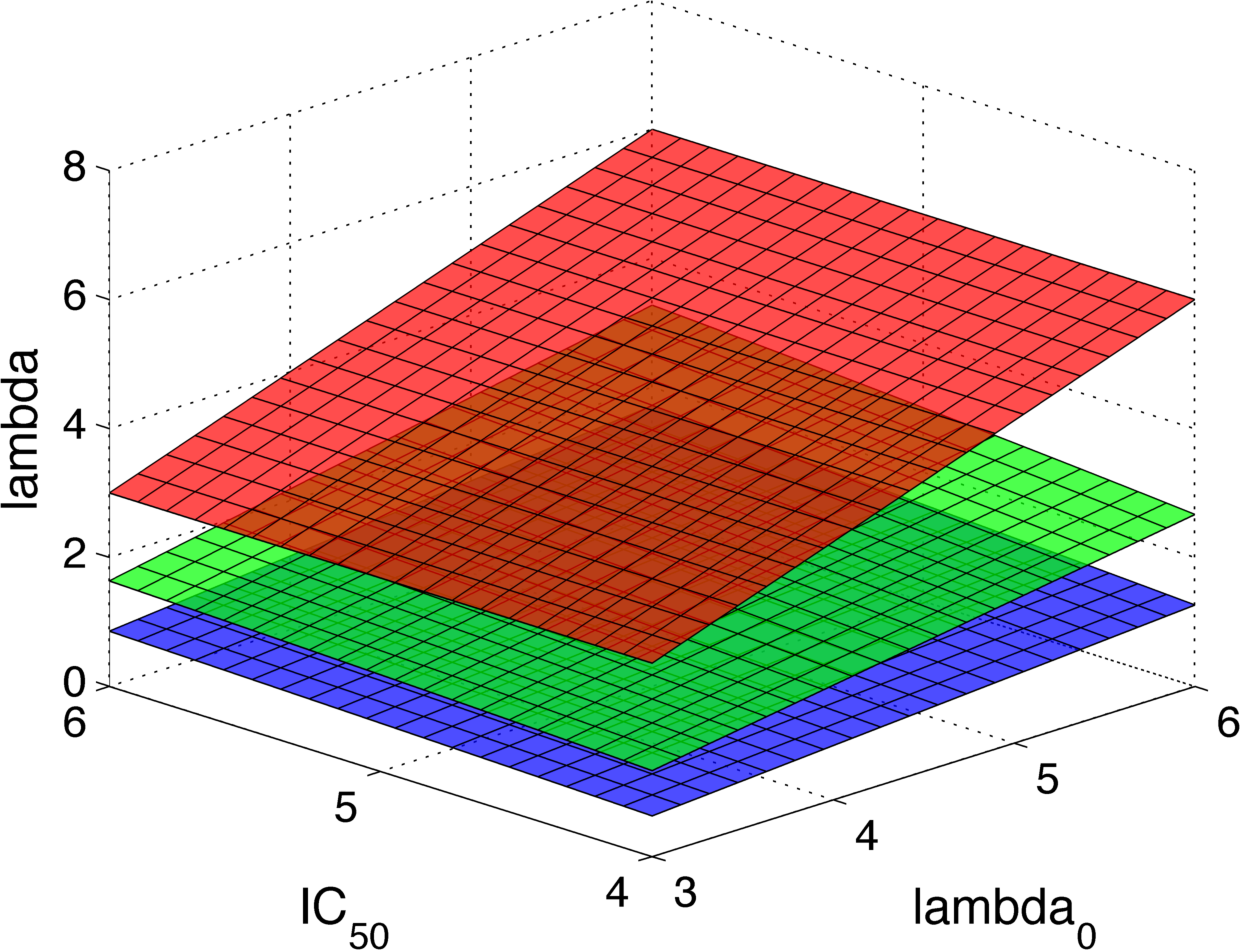
\includegraphics[width=.45\textwidth]{pics/CTS4_lambda_threeSurfaces} & 
\raisebox{0\height}{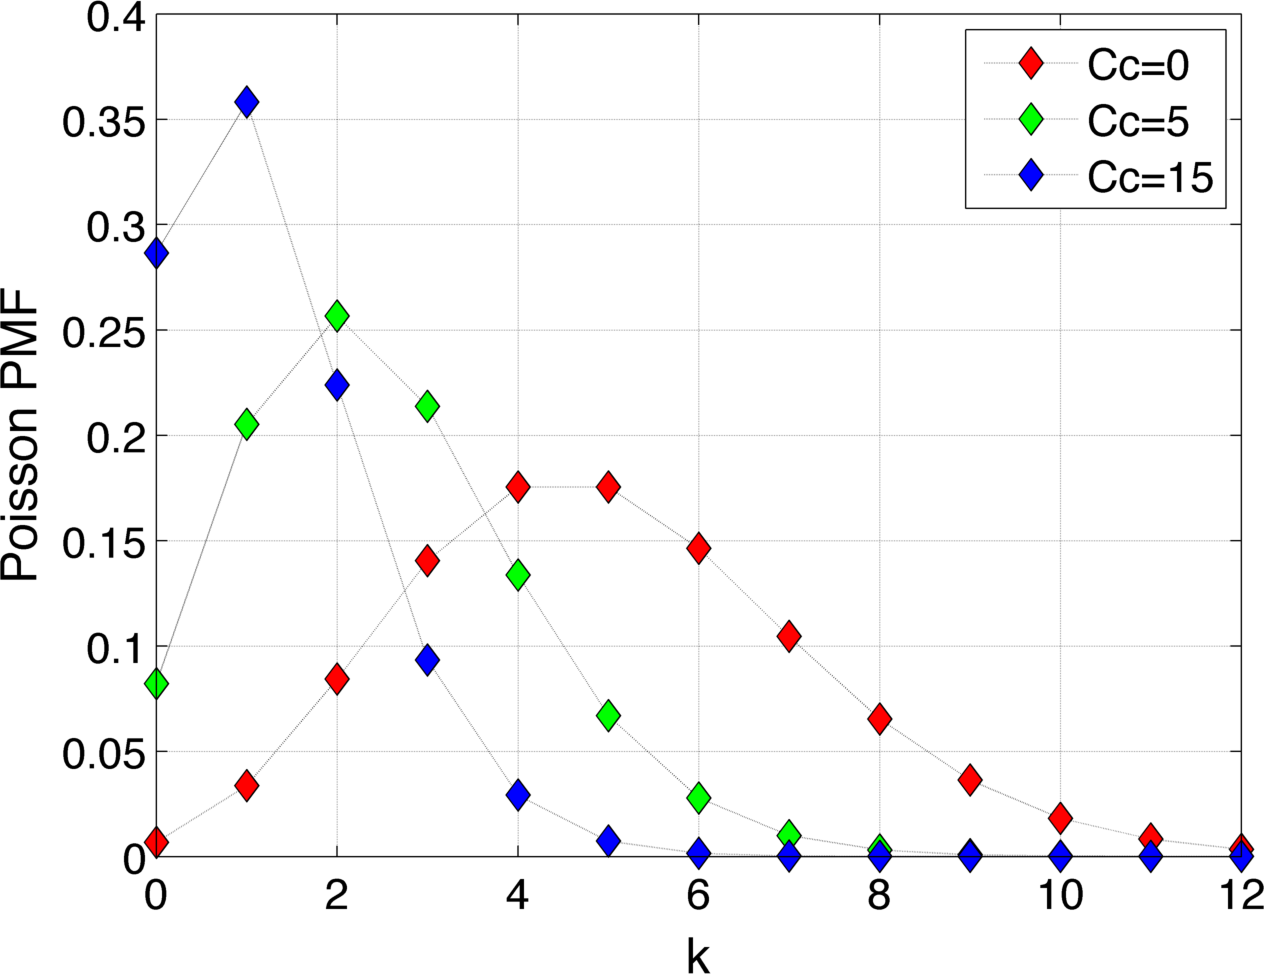
\includegraphics[scale=0.45]{pics/CTS4_poissonScan}}
\end{tabular}
\caption{(LEFT) $\lambda$--surface as function of $\lambda0$ and $IC50$ plotted for $Cc = \{1,5,15\}$. (RIGHT) Poisson PMF for fixed parameters $\lambda0 = IC50 = 5$ and varying concentration $Cc = \{1,5,15\}$.}
\label{fig:lambdasurface}
\end{figure}


%%%%%%%%%%%%%%%%%%%%%%%%%%%%%%%%%%%%%%%%%%%%%%%%%%%%%%%%%%%%%%%%
\subsubsection{Model description}
\label{subsec:exp5_TaskDescription}

%\paragraph{Individual parameters model}
%
%Details omitted here...
%
%\begin{eqnarray}
%ka& \sim& \mbox{logNormal}(ka_{\rm pop}, \omega_{ka});  \quad ka_{\rm pop}=1,\quad \omega_{ka}=0.6 \nonumber \\
%V& \sim& \mbox{logNormal}(V_{\rm pop}, \omega_{V}); \quad V_{\rm pop}=8,\quad \omega_V=0.2 \nonumber \\
%CL& \sim&  \mbox{logNormal}(CL_{\rm pop}, \omega_{CL}); \quad CL_{\rm pop}=0.13,\quad \omega_{CL}=0.2 \nonumber \\
%\lambda0 & \sim&  \mbox{logNormal}(\lambda0_{{\rm pop}}, \omega_{\lambda0}); \quad  \lambda0_{{\rm pop}} = 5, \quad \omega_{\lambda0} = 0.2 \nonumber \\
%IC50 &\sim& \mbox{logNormal}(IC50_{{\rm pop}}, \omega_{IC50}); \quad  IC50_{{\rm pop}} = 5, \quad \omega_{IC50} = 0 \nonumber
%\end{eqnarray}
%\begin{eqnarray}
%\log(V_i) &=& \log(V_{pop}) + \beta_{1,V}\log(W_i/70) + \eta_{V,i} \nonumber \\
%\log(CL_i) &=& \log(CL_{pop}) + \beta_{1,CL}\log(W_i/70) + \eta_{CL,i} \nonumber \\
%\beta_{1,V}&=&1 \nonumber \\
%\beta_{1,CL}&=&0.75 \nonumber \\
%\rho_{V,CL}&=&0.7 \mbox{  (the correlation coefficient between } \eta_{V,i} \mbox{ and } \eta_{CL,i}  \mbox{)} \nonumber
%\end{eqnarray}


\paragraph{Structural model}
\begin{eqnarray}
\frac{dAd}{dt} &=&-ka \times Ad \nonumber \\
\frac{dAc}{dt}&=&ka \times Ad - k \times Ac \nonumber \\ 
Cc &=& Ac/V \nonumber \\ \nonumber
\end{eqnarray}
\paragraph{Observation model}

\begin{itemize}
\item
Data type: discrete/count 
\item
Count variable: $Y$
\item
log(Poisson PMF)
\begin{align}
& Log(P(Y=k)) = -\lambda + k\times log(\lambda) - \log(k!) \nonumber
\end{align}
\item
Rate parameter $\lambda$, the Poisson 'intensity' is function of drug concentration, $Cc$
\begin{align}
& \lambda = \lambda0 (1 - Cc/(IC50 + Cc)) \nonumber
\end{align}
\end{itemize}

\subsubsection{PharmML code}
The code below covers the Observation model with eqs.(\ref{eq:logPMF}) and (\ref{eq:lambda}).
All parameters are assumed to be defined in the \xelem{ParameterModel}.
\lstset{language=XML}
\begin{lstlisting}
        <ObservationModel blkId="om1">
            <Discrete>
                <CountData>
                    <CountVariable symbId="k"/>
                    
                    <!-- Poisson intensity - function of drug concentration, Cc -->                    
                    <IntensityParameter symbId="Lambda">
                        <ct:Assign>
                            <math:Equation>
                                <math:Binop op="times">
                                    <ct:SymbRef blkIdRef="pm1" symbIdRef="lambda0"/>
                                    <math:Binop op="minus">
                                        <ct:Real>1</ct:Real>
                                        <math:Binop op="divide">
                                            <ct:SymbRef blkIdRef="sm1" symbIdRef="Cc"/>
                                            <math:Binop op="plus">
                                                <ct:SymbRef blkIdRef="pm1" symbIdRef="IC50"/>
                                                <ct:SymbRef blkIdRef="sm1" symbIdRef="Cc"/>
                                            </math:Binop>
                                        </math:Binop>
                                    </math:Binop>
                                </math:Binop>
                            </math:Equation>
                        </ct:Assign>
                    </IntensityParameter>
                    
                    <!-- log(P(Y=k)) = -lambda+k*log(lambda)-log(k!) -->
                    <PMF linkFunction="log">
                        <math:LogicBinop op="eq">
                            <ct:SymbRef symbIdRef="Y"/>
                            <ct:SymbRef symbIdRef="k"/>
                        </math:LogicBinop>
                        <PoissonDistribution xmlns="http://www.uncertml.org/3.0" 
                            definition="http://www.uncertml.org/3.0">
                            <rate>
                                <var varId="Lambda"/>
                            </rate>
                        </PoissonDistribution>
                    </PMF>
                </CountData>
            </Discrete>
        </ObservationModel>
\end{lstlisting}






%\subsubsection{Poisson model}
%
%\subsubsection{NM-TRAN code provided by Nick Holford and Mike Smith}
%\begin{lstlisting}
%$PROB Count data
%$DATA ..\count_sim.std\count_sim.fit IGNORE @
%$INPUT ID TIME CMTX AMT RATX WT AGE SEX TYPE CP DV MDV
%;$SIM (20000321 NEW) (1234567 UNIFORM) SUBPROBLEMS=1
%$ESTIM MAXEVAL=9990 METHOD=COND LAPLACE -2LL NOABORT
% 
%$THETA
% 
%(0,1) FIX    ; pop_cl
%(1,10) FIX ; pop_v
%(0,0.5) FIX ; pop_ka
%(0,10,)      ; BaseCount
%(0,.5,10)    ; Beta
% 
%$OMEGA
%0.09 FIX ; ppv_cl
%0.09 FIX ; ppv_v
%0.09 FIX ; ppv_ka
%0.04 ; ppv_event
% 
%$SUBROUTINE ADVAN=2 TRAN=2
% 
%$PK
%     GRPCL  = POP_CL
%     GRPV   = POP_V
%     GRPKA  = POP_KA
%     
%     PPVCL  = PPV_CL
%     PPVV   = PPV_V
%     PPVKA  = PPV_KA
% 
%     CL     = GRPCL*EXP(PPVCL)
%     V      = GRPV*EXP(PPVV)
%     KA     = GRPKA*EXP(PPVKA)
%      
%     S2     = V
%     REPI   = IREP
%      
%$ERROR
%; Drug effect
% 
%COUNT=BaseCount + Beta*CP + ppv_event
% 
%;Stirlings formula for log DV factorial
%IF (DV.GT.0) THEN
%      LDVFAC=(DV+.5)*LOG(DV)-DV+.5*LOG(6.283185)
%ELSE
%      LDVFAC=0
%ENDIF
% 
%Y=-2*(-COUNT+DV*LOG(COUNT)-LDVFAC)
% 
%;$TABLE ID TIME CMTX AMT RATX WT AGE SEX TYPE CP MDV COUNT
%;NOPRINT FILE=count.fit
%\end{lstlisting}



%\subsubsection{Poisson model - P}
%\paragraph{NM-TRAN code provided by Elodie Plan}
%\begin{lstlisting}
%\end{lstlisting}
%\paragraph{MLXTRAN code from Monolix 4.1 User Manual}
%\begin{lstlisting}
%\end{lstlisting}
%
%
%\begin{sidewaystable}[h]
%\caption{Performance After Post Filtering}  % title name of the table
%\centering  % centering table
%\begin{tabular}{l c c rrrrrrr}  % creating 10 columns
%\hline\hline                       % inserting double-line
% Audio &Audibility & Decision &\multicolumn{7}{c}{Sum of Extracted Bits} 
%\\ [0.5ex]   
%\hline              % inserts single-line
%% Entering 1st row
% & &soft &1 & $-1$ & 1 & 1 & $-1$ & $-1$ & 1  \\[-1ex]
%\raisebox{1.5ex}{Police} & \raisebox{1.5ex}{5}&hard
%&  2 & $-4$ & 4 & 4 & $-2$ & $-4$ & 4 \\[1ex]
%% Entering 2nd row
%& &soft & 1 & $-1$ & 1 & 1 & $-1$ & $-1$ & 1  \\[-1ex]
%\raisebox{1.5ex}{Beethoven} & \raisebox{1.5ex}{5}& hard
%&8 & $-8$ & 2 & 8 & $-8$ & $-8$ & 6 \\[1ex]
%% Entering 3rd row
%& &soft & 1 & $-1$ & 1 & 1 & $-1$ & $-1$ & 1  \\[-1ex]
%\raisebox{1.5ex}{Metallica} & \raisebox{1.5ex}{5}& hard
%&4 & $-8$ & 8 & 4 & $-8$ & $-8$ & 8  \\[1ex]
%% [1ex] adds vertical space
%\hline                          % inserts single-line
%\end{tabular}
%\label{tab:LPer}
%\end{sidewaystable}
%


\newpage
% INPUT
\section{Categorical data models}
\label{subsec:categoricalDataModels}


%%%%%%%%%%%%%%%%%%%%%%%%%%%%%%%%%%%%%%%%%%%%%%%%%%%%%%%%%%%%%%%%
\subsection{Binomial distribution}

\paragraph{Observation model}
	
\begin{itemize}
\item
Type of observed variable -- discrete/categorical
\item
Category variable: $y$
\item
Set of categories: $\{0,1\}$
\item
Probability for category '1'
\begin{eqnarray}
&& P(y=1) = p \nonumber
\end{eqnarray}
\end{itemize}


\subsubsection{NM-TRAN code:}
\myStartLine
\lstset{language=NONMEMdataSet}
\begin{lstlisting}
$PROB Binary model

$INPUT ID TIME DV

$DATA data.csv IGNORE=@ 

$PRED
  TVBASE = THETA(1)                      ; TVBASE is a proportion
  PHI    = LOG(TVBASE/(1-TVBASE)) + ETA(1)  
  BASE   = EXP(PHI)/(1+EXP(PHI))   ; Logit transformation, 0<BASE<1

  IF(DV.GT.1) THEN   ; A event for binary data
    Y=BASE
    RDV = 1     ; the "real" DV
  ENDIF
  IF(DV.LE.1) THEN   ; No event for binary data
    Y=1-BASE
    RDV = 0     ; the "real" DV
  ENDIF

$THETA (0,.8)    ; BASE
$OMEGA 0.1       ; BSV BASE

$ESTIM MAXEVAL=9999 METHOD=COND LAPLACE LIKE PRINT=1 MSFO=msfb
\end{lstlisting}
\myEndLine

\subsubsection{MLXTRAN code:}
Code source: Lixoft MLXTRAN tutorial.

\myStartLine
\lstset{language=MLXTRANcode}
\begin{lstlisting}
DESCRIPTION:
Categorical data model - Binomial distribution

INPUT:
parameter = p

OBSERVATION:
y= { 
	type = categorical 
	categories = {0,1} 
	P(y=1) = p 
}

OUTPUT:
output = y
\end{lstlisting}
\myEndLine

\subsubsection{PharmML code:}

\lstset{language=XML}
\begin{lstlisting}
        <ObservationModel blkId="om1">
            <Discrete>
                <CategoricalData ordered="no">
                    <SimpleParameter symbId="p"/>
                    
                    <ListOfCategories> 
                        <Category symbId="cat0"/>
                        <Category symbId="cat1"/>
                    </ListOfCategories>
                    
                    <CategoryVariable symbId="y"/>
                    
                    <!-- P(y = 1) = p -->
                    <ProbabilityAssignment>
                        <Probability linkFunction="identity">
                            <math:LogicBinop op="eq">
                                <ct:SymbRef symbIdRef="y"/>
                                <ct:SymbRef symbIdRef="cat1"/>
                            </math:LogicBinop>
                        </Probability>
                        <ct:Assign>
                            <ct:SymbRef symbIdRef="p"/>
                        </ct:Assign>
                    </ProbabilityAssignment>
                </CategoricalData>
            </Discrete>
        </ObservationModel>
\end{lstlisting}


\subsubsection{PharmML code -- alternative using UncertML:}

\lstset{language=XML}
\begin{lstlisting}
        <ObservationModel blkId="om1">
            <Discrete>
                <CategoricalData ordered="no">
                    <SimpleParameter symbId="p"/>
                    
                    <ListOfCategories> 
                        <Category symbId="cat0"/>
                        <Category symbId="cat1"/>
                    </ListOfCategories>
                    
                    <CategoryVariable symbId="y"/>
                    
                    <PMF linkFunction="identity">
                        <BernoulliDistribution xmlns="http://www.uncertml.org/3.0" 
                            definition="http://www.uncertml.org/3.0">
                            <categoryProb definition="http://www.uncertml.org/3.0">
                                <name>cat1</name>
                                <probability>
                                    <var varId="p"/>
                                </probability>
                            </categoryProb>
                        </BernoulliDistribution>
                    </PMF>
                </CategoricalData>
            </Discrete>
        </ObservationModel>
\end{lstlisting}


%%%%%%%%%%%%%%%%%%%%%%%%%%%%%%%%%%%%%%%%%%%%%%%%%%%%%%%%%%%%%%%%
\subsection{Binomial distribution with Markovian dependence}

\paragraph{Observation model}

% TEMPLATE for CATEGORICAL MODEL DESCRIPTION
\begin{itemize}
\item
Type of observed variable -- discrete/categorical
\item
Category variable: $y$
\item
Previous state variable: $yp$
\item
Set of categories: $\{0,1\}$
\item
Probability for category '1'
\begin{align}
& P(y=1) = p \nonumber
\end{align}
\item
Markov dependance with transition probabilities:
\begin{itemize}
\item
$P(y=1 | yp=0) = p01$ and 
\item
$P(y=1 | yp=1) = p11$
\end{itemize}
\end{itemize}

\begin{figure}[htbp!]
\includegraphics[width=.75\textwidth]{pics/binomialMarkov} 
\caption{Markov transition probabilities for two-states model.}
\label{fig:binomialMarkov}
\end{figure}


\subsubsection{NM-TRAN code:}

\myStartLine
\lstset{language=NONMEMdataSet}
\begin{lstlisting}
$PROB Transition probabilities

$INPUT ID TIME DV PDV ;PDV=value of preceding observation

$DATA data.csv IGNORE=@ 

$PRED

  TVP10 = THETA(1)                    
  PHI1    = LOG(TVP10/(1-TVP10)) + ETA(1)  
  P10   = EXP(PHI1)/(1+EXP(PHI1))
  
  TVP01 = THETA(2)                    
  PHI0    = LOG(TVP01/(1-TVP01)) + ETA(2)  
  P01   = EXP(PHI0)/(1+EXP(PHI0))
   
   IF(PDV.EQ.0.AND.DV.EQ.1) Y=P10
   IF(PDV.EQ.0.AND.DV.EQ.0) Y=1-P10 
   IF(PDV.EQ.1.AND.DV.EQ.0) Y=P01 
   IF(PDV.EQ.1.AND.DV.EQ.1) Y=1-P01 
   
$THETA  (0,.1,1)   
$THETA  (0,.1,1)   
$OMEGA 0.1 
$OMEGA 0.1  

$ESTIM MAXEVAL=9999 METHOD=COND LAPLACE LIKE PRINT=1 MSFO=msfb
\end{lstlisting}
\myEndLine

\subsubsection{MLXTRAN code:}
Code provided by Marc Lavielle. 

\myStartLine
\lstset{language=MLXTRANcode}
\begin{lstlisting}
DESCRIPTION:
Categorical data model with Markovian dependence, Binomial distribution

INPUT:
parameter = {p01, p11}

OBSERVATION:
y = {
      type = categorical
      categories = {0,1}
      dependence = Markov
      P(y=1 | yp=0) = p01
      P(y=1 | yp=1) = p11
}

OUTPUT:
output = y
\end{lstlisting}
\myEndLine

\subsubsection{PharmML code:}

\lstset{language=XML}
\begin{lstlisting}
        <ObservationModel blkId="om1">
            <Discrete>
                <CategoricalData ordered="no">
                    <SimpleParameter symbId="p01"/>
                    <SimpleParameter symbId="p11"/>
                    
                    <ListOfCategories> 
                        <Category symbId="cat0"/>
                        <Category symbId="cat1"/>
                    </ListOfCategories>
                    
                    <CategoryVariable symbId="y"/>
                    <PreviousStateVariable symbId="yp"/>
                    
                    <Dependance type="discreteMarkov"/>
                    
                    <!-- P(y=1|yp=0)=p01 -->
                    <ProbabilityAssignment>
                        <Probability>
                            <CurrentState>
                                <math:LogicBinop op="eq">
                                    <ct:SymbRef symbIdRef="y"/>
                                    <ct:SymbRef symbIdRef="cat1"/>
                                </math:LogicBinop>
                            </CurrentState>
                            <PreviousState>
                                <math:LogicBinop op="eq">
                                    <ct:SymbRef symbIdRef="yp"/>
                                    <ct:SymbRef symbIdRef="cat0"/>
                                </math:LogicBinop>
                            </PreviousState>
                        </Probability>
                        <ct:Assign>
                            <ct:SymbRef symbIdRef="p01"/>
                        </ct:Assign>
                    </ProbabilityAssignment>
                    
                    <!-- P(y=1|yp=1)=p11-->
                    <ProbabilityAssignment>
                        <Probability>
                            <CurrentState>
                                <math:LogicBinop op="eq">
                                    <ct:SymbRef symbIdRef="y"/>
                                    <ct:SymbRef symbIdRef="cat1"/>
                                </math:LogicBinop>
                            </CurrentState>
                            <PreviousState>
                                <math:LogicBinop op="eq">
                                    <ct:SymbRef symbIdRef="yp"/>
                                    <ct:SymbRef symbIdRef="cat1"/>
                                </math:LogicBinop>
                            </PreviousState>
                        </Probability>
                        <ct:Assign>
                            <ct:SymbRef symbIdRef="p11"/>
                        </ct:Assign>
                    </ProbabilityAssignment>
                </CategoricalData>
            </Discrete>
        </ObservationModel>
\end{lstlisting}


%%%%%%%%%%%%%%%%%%%%%%%%%%%%%%%%%%%%%%%%%%%%%%%%%%%%%%%%%%%%%%%%
\subsection{Explicit probabilities per category -- three categories}

\paragraph{Observation model}

\begin{itemize}
\item
Type of observed variable -- discrete/categorical
\item
Category variable: $y$
\item
Set of categories: $\{1,2,3\}$
\item
Probabilities for category '1' and '2'
\begin{eqnarray}
&& P(y=1) = a1/(a1+a2+a3)  \nonumber \\
&& P(y=2) = a2/(a1+a2+a3)  \nonumber 
\end{eqnarray}
\end{itemize}


\subsubsection{NM-TRAN code:}

\myStartLine
\lstset{language=NONMEMdataSet}
\begin{lstlisting}
	missing
\end{lstlisting}
\myEndLine

\subsubsection{MLXTRAN code:}
Code source: Lixoft MLXTRAN tutorial.

\myStartLine
\lstset{language=MLXTRANcode}
\begin{lstlisting}
DESCRIPTION:
Categorical data model - 3 categories

INPUT:
parameter = {a1, a2, a3}

OBSERVATION:
y = {
	type = categorical 
	categories = {1, 2, 3} 
	P(y=1) = a1/(a1+a2+a3) 
	P(y=2) = a2/(a1+a2+a3) 
}

OUTPUT:
output = y
\end{lstlisting}
\myEndLine

\textit{ALTERNATIVELY} (for $P(y=1)$ and $P(y=3)$):

\begin{lstlisting}
OBSERVATION:
y = { 
	type = categorical 
	categories = {1, 2, 3} 
	P(y=1) = a1/(a1+a2+a3) 
	P(y=3) = a3/(a1+a2+a3) 
}
\end{lstlisting}

\subsubsection{PharmML code:}

\lstset{language=XML}
\begin{lstlisting}
        <ObservationModel blkId="om1">
            <Discrete>
                <CategoricalData ordered="no">
                    <SimpleParameter symbId="a1"/>
                    <!-- a1, a2 omitted -->
                    
                    <ListOfCategories> 
                        <Category symbId="cat1"/>
                        <Category symbId="cat2"/>
                        <Category symbId="cat3"/>
                    </ListOfCategories>
                    
                    <CategoryVariable symbId="y"/>
                    
                    <!-- P(y = 1) = a1/(a1+a2+a3) -->
                    <ProbabilityAssignment>
                        <Probability linkFunction="identity">
                            <math:LogicBinop op="eq">
                                <ct:SymbRef symbIdRef="y"/>
                                <ct:SymbRef symbIdRef="cat1"/>
                            </math:LogicBinop>
                        </Probability>
                        <ct:Assign>
                            <math:Equation>
                                <math:Binop op="divide">
                                    <ct:SymbRef symbIdRef="a1"/>
                                    <math:Binop op="plus">
                                        <ct:SymbRef symbIdRef="a1"/>
                                        <math:Binop op="plus">
                                            <ct:SymbRef symbIdRef="a2"/>
                                            <ct:SymbRef symbIdRef="a3"/>
                                        </math:Binop>
                                    </math:Binop>
                                </math:Binop>
                            </math:Equation>
                        </ct:Assign>
                    </ProbabilityAssignment>
                    
                    <!-- P(y = 2) = a2/(a1+a2+a3) -->
                    <ProbabilityAssignment>
                        <Probability linkFunction="identity"> 
                            <math:LogicBinop op="eq">
                                <ct:SymbRef symbIdRef="y"/>
                                <ct:SymbRef symbIdRef="cat2"/>
                            </math:LogicBinop>
                        </Probability>
                        <ct:Assign>
                            <math:Equation>
                                <math:Binop op="divide">
                                    <ct:SymbRef symbIdRef="a2"/>
                                    <math:Binop op="plus">
                                        <ct:SymbRef symbIdRef="a1"/>
                                        <math:Binop op="plus">
                                            <ct:SymbRef symbIdRef="a2"/>
                                            <ct:SymbRef symbIdRef="a3"/>
                                        </math:Binop>
                                    </math:Binop>
                                </math:Binop>
                            </math:Equation>
                        </ct:Assign>
                    </ProbabilityAssignment>
                </CategoricalData>
            </Discrete>
        </ObservationModel>
\end{lstlisting}


%%%%%%%%%%%%%%%%%%%%%%%%%%%%%%%%%%%%%%%%%%%%%%%%%%%%%%%%%%%%%%%%
\subsection{Cumulative probabilities -- three categories}

\paragraph{Observation model}

\begin{itemize}
\item
Type of observed variable -- discrete/categorical
\item
Category variable: $y$
\item
Set of categories: $\{1,2,3\}$
\item
Cumulative probabilities
\begin{eqnarray}
&& P(y<=1) = a1/(a1+a2+a3) \nonumber \\
&& P(y<=2) = (a1+a2)/(a1+a2a31)  \nonumber 
\end{eqnarray}
\end{itemize}


\subsubsection{NM-TRAN code:}

\myStartLine

\lstset{language=NONMEMdataSet}
\begin{lstlisting}
	missing
\end{lstlisting}

\myEndLine

\subsubsection{MLXTRAN code:}
Code source: Monolix 4.1 User Manual.

\myStartLine

\lstset{language=MLXTRANcode}
\begin{lstlisting}
DESCRIPTION:
Ordered categorical data model - 3 categories Cumulative probabilities

INPUT:
parameter = {a1, a2, a3}

OBSERVATION:
y = { 
	type = categorical 
	categories = {1, 2, 3} 
	P(y<=1) = a1/(a1+a2+a3) 
	P(y<=2) = (a1+a2)/(a1+a2a31) 
}

OUTPUT:
output = y
\end{lstlisting}

\myEndLine

\subsubsection{PharmML code:}

\lstset{language=XML}
\begin{lstlisting}
        <ObservationModel blkId="om1">
            <Discrete>
                <CategoricalData ordered="yes">
                    <SimpleParameter symbId="a1"/>
                    <SimpleParameter symbId="a2"/>
                    <SimpleParameter symbId="a3"/>
                    
                    <ListOfCategories> 
                        <Category symbId="cat1"/>
                        <Category symbId="cat2"/>
                        <Category symbId="cat3"/>
                    </ListOfCategories>
                    
                    <CategoryVariable symbId="y"/>
                    
                    <!-- P(y <= 1) = a1/(a1+a2+a3) --> 
                    <ProbabilityAssignment>
                        <Probability linkFunction="identity">
                            <math:LogicBinop op="leq">
                                <ct:SymbRef symbIdRef="y"/>
                                <ct:SymbRef symbIdRef="cat1"/>
                            </math:LogicBinop>
                        </Probability>
                        <ct:Assign>
                            <math:Equation>
                                <math:Binop op="divide">
                                    <ct:SymbRef symbIdRef="a1"/>
                                    <math:Binop op="plus">
                                        <ct:SymbRef symbIdRef="a1"/>
                                        <math:Binop op="plus">
                                            <ct:SymbRef symbIdRef="a2"/>
                                            <ct:SymbRef symbIdRef="a3"/>
                                        </math:Binop>
                                    </math:Binop>
                                </math:Binop>
                            </math:Equation>
                        </ct:Assign>
                    </ProbabilityAssignment>
                    
                    <!-- P(y <= 2) = a2/(a1+a2+a3) -->
                    <ProbabilityAssignment>
                        <Probability linkFunction="identity">
                            <math:LogicBinop op="leq">
                                <ct:SymbRef symbIdRef="y"/>
                                <ct:SymbRef symbIdRef="cat2"/>
                            </math:LogicBinop>
                        </Probability>
                        <ct:Assign>
                            <math:Equation>
                                <math:Binop op="divide">
                                    <ct:SymbRef symbIdRef="a2"/>
                                    <math:Binop op="plus">
                                        <ct:SymbRef symbIdRef="a1"/>
                                        <math:Binop op="plus">
                                            <ct:SymbRef symbIdRef="a2"/>
                                            <ct:SymbRef symbIdRef="a3"/>
                                        </math:Binop>
                                    </math:Binop>
                                </math:Binop>
                            </math:Equation>
                        </ct:Assign>
                    </ProbabilityAssignment>
                </CategoricalData>
            </Discrete>
        </ObservationModel>
\end{lstlisting}


%\subsubsection{Tail probabilities - three categories}
%\paragraph{NM-TRAN code provided by ...}
%%\begin{lstlisting}
%%\end{lstlisting}
%\paragraph{MLXTRAN code from Monolix 4.1 User Manual}
%\begin{lstlisting}
%DESCRIPTION:
%Ordered categorical data model - 3 categories Tail probabilities
%
%INPUT:
%parameter = {a1, a2, a3}
%
%OBSERVATION:
%y= { type = categorical 
%categories = {1, 2, 3} 
%P(y>1) = (a2+a3)/(a1+a2+a3) 
%P(y>2) = a3/(a1+a2+a3) }
%
%OUTPUT:
%output = y
%\end{lstlisting}


%%%%%%%%%%%%%%%%%%%%%%%%%%%%%%%%%%%%%%%%%%%%%%%%%%%%%%%%%%%%%%%%
\subsection{Cumulative logit probabilities -- three categories}

\paragraph{Observation model}

\begin{itemize}
\item
Type of observed variable -- discrete/categorical
\item
Category variable: $y$
\item
Set of categories: $\{1,2,3\}$
\item
Cumulative logits
\begin{align}
& \text{logit}(P(y<=1) )= \theta1  \nonumber \\
& \text{logit}(P(y<=2) )= \theta1+ \theta2  \nonumber 
\end{align}
\end{itemize}


\subsubsection{NM-TRAN code:}

\myStartLine

\lstset{language=NONMEMdataSet}
\begin{lstlisting}
	missing
\end{lstlisting}

\myEndLine

\subsubsection{MLXTRAN code:}
Code source: Monolix 4.1 User Manual

\myStartLine

\lstset{language=MLXTRANcode}
\begin{lstlisting}
DESCRIPTION:
Ordered categorical data model - 3 categories Logit - probabilities

INPUT:
parameter = {theta1, theta2}

OBSERVATION:
y = {
	type = categorical 
	categories = {1, 2, 3} 
	logit(P(y<=1))= theta1 
	logit(P(y<=2))= theta1+theta2
}
OUTPUT:
output = y


ALTERNATIVELY with tails

OBSERVATION:
y = { 
	type = categorical 
	categories = {1, 2, 3} 
	logit(P(t>1))= -theta1 
	logit(P(t>2))= -theta1-theta2
}
\end{lstlisting}

\myEndLine

\subsubsection{PharmML code:}

\lstset{language=XML}
\begin{lstlisting}
        <ObservationModel blkId="om1">
            <Discrete>
                <CategoricalData ordered="yes">
                    <SimpleParameter symbId="theta1"/>
                    <SimpleParameter symbId="theta2"/>
                    
                    <ListOfCategories> 
                        <Category symbId="cat1"/>
                        <Category symbId="cat2"/>
                    </ListOfCategories>
                    
                    <CategoryVariable symbId="y"/>
                    
                    <!-- logit(P(y <= 1)) = theta1 -->
                    <ProbabilityAssignment>
                        <Probability linkFunction="logit">
                            <math:LogicBinop op="leq">
                                <ct:SymbRef symbIdRef="y"/>
                                <ct:SymbRef symbIdRef="cat1"/>
                            </math:LogicBinop>
                        </Probability>
                        <ct:Assign>
                            <ct:SymbRef symbIdRef="theta1"/>
                        </ct:Assign>
                    </ProbabilityAssignment>
                    
                    <!-- logit(P(y <= 2)) = theta1 + theta2 -->
                    <ProbabilityAssignment>
                        <Probability linkFunction="logit">
                            <math:LogicBinop op="leq">
                                <ct:SymbRef symbIdRef="y"/>
                                <ct:SymbRef symbIdRef="cat2"/>
                            </math:LogicBinop>
                        </Probability>
                        <ct:Assign>
                            <math:Equation>
                                <math:Binop op="plus">
                                    <ct:SymbRef symbIdRef="theta1"/>
                                    <ct:SymbRef symbIdRef="theta2"/>
                                </math:Binop>
                            </math:Equation>
                        </ct:Assign>
                    </ProbabilityAssignment>
                </CategoricalData>
            </Discrete>
        </ObservationModel>
 \end{lstlisting}



%%%%%%%%%%%%%%%%%%%%%%%%%%%%%%%%%%%%%%%%%%%%%%%%%%%%%%%%%%%%%%%%
\subsection{Tail logit probabilities}

\paragraph{Observation model}

\begin{itemize}
\item
Type of observed variable -- discrete / ordered categorical
\item
Category variable: $y$
\item
Set of categories: $\{0,1,2,3\}$
\item
Tail logits
\begin{align}
& \text{logit}(P(y \ge 0)) = B1 + \eta1 \nonumber \\
& \text{logit}(P(y \ge 1)) = B1 + B2 + \eta1 \nonumber \\
& \text{logit}(P(y \ge 2)) = B1 + B2 + B3 + \eta1 \nonumber 
\end{align}
with $\eta1 \sim N(0, \omega1)$.
\end{itemize}


\subsubsection{NM-TRAN code:}
Code example provided by Mats Karlsson.

\myStartLine

\lstset{language=NONMEMdataSet}
\begin{lstlisting}
$PROB mixed-effect Ordered Categorical, baseline model
$INPUT ID TIME ODV DOSE ICL IV IKA 
       TYPE SMAX DV=SMXH THR CAV CAVH CON
       ;CNT CNT2 CNT3 HC HC2 HC3 
       ;ETA1 ETA2 ETA3 ETA4

$DATA data.csv IGNORE=@ ACCEPT=(THR.GT.0)

$PRED
  ;Baseline values
  B1 = THETA(1)
  B2 = THETA(2)
  B3 = THETA(3)

  ;Logits for Y>=1, Y>=2, Y>=3
  LGE1 = B1+ETA(1)
  LGE2 = B1+B2+ETA(1)
  LGE3 = B1+B2+B3+ETA(1)

  ;Probabilities for Y>=2, Y>=3
  PGE1 = EXP(LGE1)/(1+EXP(LGE1))
  PGE2 = EXP(LGE2)/(1+EXP(LGE2))
  PGE3 = EXP(LGE3)/(1+EXP(LGE3))

  ;Probabilities for Y=0, Y=1, Y=2, Y=3
  P0 = (1-PGE1) 
  P1 = (PGE1-PGE2)
  P2 = (PGE2-PGE3)
  P3 = PGE3   
 
  ;Select appropriate P(Y=m)
  IF(DV.EQ.0) Y=P0
  IF(DV.EQ.1) Y=P1
  IF(DV.EQ.2) Y=P2
  IF(DV.EQ.3) Y=P3

$THETA (0.63)          ; B1
$THETA (-INF,-.1,0)    ; B2
$THETA (-INF,-.1,0)    ; B3
$OMEGA .1


$ESTIM MAXEVAL=9990 METHOD=COND LAPLACE LIKE PRINT=1 MSFO=msfb45
$COV PRINT=E

$TABLE ID TIME NOPRINT ONEHEADER FILE=sdtab45
$TABLE ID CAV CAVH CON NOPRINT ONEHEADER FILE=cotab45
$TABLE ID DOSE NOPRINT ONEHEADER FILE=catab45
$TABLE ID ICL IV IKA NOPRINT ONEHEADER FILE=patab45
\end{lstlisting}

\myEndLine

\subsubsection{MLXTRAN code:}

\myStartLine

\lstset{language=MLXTRANcode}
\begin{lstlisting}
DESCRIPTION: Ordered categorical model with tail probabilities

[INDIVIDUAL]
INPUT:
parameter = {B1_POP ,B1_OMEGA}

DEFINITION:
B1 =  {distribution=logNormal, mean= B1_POP, sd=B1_OMEGA}


[OBSERVATION]
INPUT:
parameter = {B1, B2, B3}

DEFINITION:
y = {
	type = categorical
	categories = {0, 1, 2, 3}
	logit(P(y>=0)) = B1
	logit(P(y>=1)) = B1 + B2
	logit(P(y>=2)) = B1 + B2 + B3
}

OUTPUT:
output = level
\end{lstlisting}

\myEndLine

\subsubsection{PharmML code:}
The code handles only the encoding of probabilities. The parameters are
defined in \xelem{ParameterModel} \emph{pm1}. $b1$ is assumed to be log-normally distributed with
$\log(b1) = \log(b1_{\rm pop}) + \eta_{b1}$, $b2$ and $b3$ are fixed.

\lstset{language=XML}
\begin{lstlisting}
        <ObservationModel blkId="om1">
            <Discrete>
                <CategoricalData ordered="yes">           
                    <!-- b1 -->
                    <!-- omitted definition with IIV -->
                    <!-- b2 -->
                    <SimpleParameter symbId="b2"/>
                    <!-- b3 -->
                    <SimpleParameter symbId="b3"/>
                    
                    <ListOfCategories> 
                        <Category symbId="cat1"/>
                        <Category symbId="cat2"/>
                        <Category symbId="cat3"/>
                    </ListOfCategories>
                    
                    <CategoryVariable symbId="y"/>
                    
                    <!-- logit(P(y >= 1)) = b1 -->
                    <ProbabilityAssignment>
                        <Probability linkFunction="logit">
                            <math:LogicBinop op="geq">
                                <ct:SymbRef symbIdRef="y"/>
                                <ct:SymbRef symbIdRef="cat1"/>
                            </math:LogicBinop>
                        </Probability>
                        <ct:Assign>
                            <ct:SymbRef symbIdRef="b1"/>
                        </ct:Assign>
                    </ProbabilityAssignment>
                    
                    <!-- logit(P(y >= 2)) = b1 + b2 --> 
                    <ProbabilityAssignment>
                        <Probability linkFunction="logit">
                            <math:LogicBinop op="geq">
                                <ct:SymbRef symbIdRef="y"/>
                                <ct:SymbRef symbIdRef="cat2"/>
                            </math:LogicBinop>
                        </Probability>
                        <ct:Assign>
                            <math:Equation>
                                <math:Binop op="plus">
                                    <ct:SymbRef symbIdRef="b1"/>
                                    <ct:SymbRef symbIdRef="b2"/>
                                </math:Binop>
                            </math:Equation>
                        </ct:Assign>
                    </ProbabilityAssignment>
                    
                    <!-- logit(P(y >= 3)) = b1 + b2 + b3 --> 
                    <ProbabilityAssignment>
                        <Probability linkFunction="logit">
                            <math:LogicBinop op="geq">
                                <ct:SymbRef symbIdRef="y"/>
                                <ct:SymbRef symbIdRef="cat3"/>
                            </math:LogicBinop>
                        </Probability>
                        <ct:Assign>
                            <math:Equation>
                                <math:Binop op="plus">
                                    <math:Binop op="plus">
                                        <ct:SymbRef symbIdRef="b1"/>
                                        <ct:SymbRef symbIdRef="b2"/>
                                    </math:Binop>
                                    <ct:SymbRef symbIdRef="b3"/>
                                </math:Binop>
                            </math:Equation>
                        </ct:Assign>
                    </ProbabilityAssignment>
                </CategoricalData>
            </Discrete>
        </ObservationModel>
\end{lstlisting}


%%%%%%%%%%%%%%%%%%%%%%%%%%%%%%%%%%%%%%%%%%%%%%%%%%%%%%%%%%%%%%%%
\subsection{Cumulative logit probabilities with Markovian dependence}

\paragraph{Observation model}

\begin{itemize}
\item
Type of observed variable -- discrete / ordered categorical
\item
Category variable: $y$
\item
Previous state variable: $yp$
\item
Set of categories: $\{1,2,3\}$
\item
Markov dependance with transition probabilities:
\begin{align}
& \text{logit}(P(y<=1 | yp=1)) = a11 \nonumber \\
& \text{logit}(P(y<=2 | yp=1)) = a11 + a12\nonumber \\
& \text{logit}(P(y<=1 | yp=2)) = a21\nonumber \\
& \text{logit}(P(y<=2 | yp=2)) = a21 + a22\nonumber \\
& \text{logit}(P(y<=1 | yp=3)) = a31\nonumber \\
& \text{logit}(P(y<=2 | yp=3)) = a31 + a32\nonumber 
\end{align}
\end{itemize}


\begin{figure}[htbp!]
\includegraphics[width=.75\textwidth]{pics/cumulLogitMarkov} 
\caption{Markov transition probabilities for three-states model.}
\label{fig:cumulLogitMarkov}
\end{figure}

\subsubsection{NM-TRAN code:}

\myStartLine

\lstset{language=NONMEMdataSet}
\begin{lstlisting}
	missing
\end{lstlisting}

\myEndLine

\subsubsection{MLXTRAN code from Monolix 4.1 User Manual:}

\myStartLine

\begin{lstlisting}
DESCRIPTION:
Categorical data model with Markovian dependence,
3 categories - logit-probabilities

INPUT:
parameter = {a11, a12, a13, a21, a22, a23, a31, a32, a33}

OBSERVATION:
y = {
      type = categorical
      categories = {1,2,3}
      dependence = Markov
      logit(P(y<=1 | yp=1)) = a11
      logit(P(y<=2 | yp=1)) = a11 + a12
      logit(P(y<=1 | yp=2)) = a21
      logit(P(y<=2 | yp=2)) = a21 + a22
      logit(P(y<=1 | yp=3)) = a31
      logit(P(y<=2 | yp=3)) = a31 + a32
}
\end{lstlisting}

\myEndLine

\subsubsection{PharmML code:}
All parameters are assumed to be defined in the \xelem{ParameterModel} \emph{pm1}.

\lstset{language=XML}
\begin{lstlisting}
        <ObservationModel blkId="om1">
            <Discrete>
                <CategoricalData ordered="yes">
                    <SimpleParameter symbId="a11"/>
                    <!-- omitted a12...a32 -->
                    <SimpleParameter symbId="a33"/>
                    
                    <ListOfCategories> 
                        <Category symbId="cat1"/>
                        <Category symbId="cat2"/>
                        <Category symbId="cat3"/>
                    </ListOfCategories>
                    
                    <CategoryVariable symbId="y"/>
                    <PreviousStateVariable symbId="yp"/>
                    
                    <Dependance type="discreteMarkov"/>
                    
                    <!--   logit(P (y <= 1|yp = 1)) = a11 -->
                    <ProbabilityAssignment>
                        <Probability linkFunction="logit">
                            <CurrentState>
                                <math:LogicBinop op="leq">
                                    <ct:SymbRef symbIdRef="y"/>
                                    <ct:SymbRef symbIdRef="cat1"/>
                                </math:LogicBinop>
                            </CurrentState>
                            <PreviousState>
                                <math:LogicBinop op="eq">
                                    <ct:SymbRef symbIdRef="yp"/>
                                    <ct:SymbRef symbIdRef="cat1"/>
                                </math:LogicBinop>
                            </PreviousState>
                        </Probability>
                        <ct:Assign>
                            <ct:SymbRef symbIdRef="a11"/>
                        </ct:Assign>
                    </ProbabilityAssignment>
                    
                    <!--  logit(P (y <= 2|yp = 1)) = a11 + a12 -->
                    <ProbabilityAssignment>
                        <Probability linkFunction="logit">
                            <CurrentState>
                                <math:LogicBinop op="leq">
                                    <ct:SymbRef symbIdRef="y"/>
                                    <ct:SymbRef symbIdRef="cat2"/>
                                </math:LogicBinop>
                            </CurrentState>
                            <PreviousState>
                                <math:LogicBinop op="eq">
                                    <ct:SymbRef symbIdRef="yp"/>
                                    <ct:SymbRef symbIdRef="cat1"/>
                                </math:LogicBinop>
                            </PreviousState>
                        </Probability>
                        <ct:Assign>
                            <math:Equation>
                                <math:Binop op="plus">
                                    <ct:SymbRef symbIdRef="a11"/>
                                    <ct:SymbRef symbIdRef="a12"/>
                                </math:Binop>
                            </math:Equation>
                        </ct:Assign>
                    </ProbabilityAssignment>
                    <!--  logit(P (y <= 1|yp = 2)) = a21 -->
                    <!-- omitted here -->
                    <!--  logit(P (y <= 2|yp = 2)) = a21 + a22 -->
                    <!-- omitted here -->
                    <!--  logit(P (y <= 1|yp = 3)) = a31 -->
                    <!-- omitted here -->
                    <!--  logit(P (y <= 2|yp = 3)) = a31 + a32 -->
                    <!-- omitted here -->
                </CategoricalData>
            </Discrete>
        </ObservationModel>
\end{lstlisting}



%%%%%%%%%%%%%%%%%%%%%%%%%%%%%%%%%%%%%%%%%%%%%%%%%%%%%%%%%%%%%%%%
\subsection{Cumulative logit probabilities with Markovian and initial probabilities}
Based on an example described in \cite{MLXTRANforMonolix:2014}. 
This model extends the previous by adding the initial probabilities for a given category.

\paragraph{Observation model}

\begin{itemize}
\item
Type of observed variable -- discrete / ordered categorical
\item
Category variable: $y$
\item
Initial state variable: $yinit$
\item
Previous state variable: $yp$
\item
Set of categories: $\{1,2,3\}$
\item
Initial probabilities
\begin{align}
& P(y=1) = a1 \nonumber \\
& P(y=2) = a2  \nonumber
\end{align}
\item
Markov dependance with transition probabilities (with $y$ -- current state, $yp$ -- previous state):
\begin{align}
& \text{logit}(P(y<=1 | yp=1)) = a11 \nonumber \\
& \text{logit}(P(y<=2 | yp=1)) = a11 + a12\nonumber \\
& \text{logit}(P(y<=1 | yp=2)) = a21\nonumber \\
& \text{logit}(P(y<=2 | yp=2)) = a21 + a22\nonumber \\
& \text{logit}(P(y<=1 | yp=3)) = a31\nonumber \\
& \text{logit}(P(y<=2 | yp=3)) = a31 + a32\nonumber 
\end{align}
\end{itemize}

\subsubsection{NM-TRAN code:}

\myStartLine

\lstset{language=NONMEMdataSet}
\begin{lstlisting}
	missing
\end{lstlisting}

\myEndLine

\subsubsection{MLXTRAN code:}

\myStartLine

\lstset{language=MLXTRANcode}
\begin{lstlisting}
DESCRIPTION:
Cumulative ordered with Markov and initial probabilities

OBSERVATION:
State = {
	type = categorical
	categories = {1,2,3}
	dependence = Markov
	P(yinit=1) = a1
	P(yinit=2) = a2
	logit(P(y<=1|yp=1)) = a11
	logit(P(y<=2|yp=1)) = a11+a12
	logit(P(y<=1|yp=2)) = a21
	logit(P(y<=2|yp=2)) = a21+a22
	logit(P(y<=1|yp=3)) = a31
	logit(P(y<=2|yp=3)) = a31+a32
}
\end{lstlisting}

\myEndLine

\subsubsection{PharmML code:}
All parameters are assumed to be defined in the \xelem{ParameterModel} \emph{pm1}.

\lstset{language=XML}
\begin{lstlisting}
        <ObservationModel blkId="om1">
            <Discrete>
                <CategoricalData ordered="yes">
                    <SimpleParameter symbId="a11"/>
                    <!-- omitted a12...a32 -->
                    <SimpleParameter symbId="a33"/>
                    
                    <ListOfCategories> 
                        <Category symbId="cat1"/>
                        <Category symbId="cat2"/>
                        <Category symbId="cat3"/>
                    </ListOfCategories>
                    
                    <CategoryVariable symbId="y"/>
                    <InitialStateVariable symbId="yinit"/>
                    <PreviousStateVariable symbId="yp"/>
                    
                    <Dependance type="discreteMarkov"/>
                    
                    <!-- P(y = 1) = a1 -->
                    <ProbabilityAssignment>
                        <Probability linkFunction="identity">
                            <math:LogicBinop op="eq">
                                <ct:SymbRef symbIdRef="yinit"/>
                                <ct:SymbRef symbIdRef="cat1"/>
                            </math:LogicBinop>
                        </Probability>
                        <ct:Assign>
                            <ct:SymbRef symbIdRef="a1"/>
                        </ct:Assign>
                    </ProbabilityAssignment>
                    
                    <!-- P(y = 2) = a2 -->
                    <ProbabilityAssignment>
                        <Probability linkFunction="identity">
                            <math:LogicBinop op="eq">
                                <ct:SymbRef symbIdRef="yinit"/>
                                <ct:SymbRef symbIdRef="cat2"/>
                            </math:LogicBinop>
                        </Probability>
                        <ct:Assign>
                            <ct:SymbRef symbIdRef="a2"/>
                        </ct:Assign>
                    </ProbabilityAssignment>
                    
                    <!--   logit(P(y <= 1|yp = 1)) = a11 -->
                    <ProbabilityAssignment>
                        <!-- omitted here, identical as in previous example -->
                    </ProbabilityAssignment>
                    
                    <!--  logit(P(y <= 2|yp = 1)) = a11 + a12 -->
                    <ProbabilityAssignment>
                        <!-- omitted here, identical as in previous example -->
                    </ProbabilityAssignment>
                    <!--  logit(P(y <= 1|yp = 2)) = a21 -->
                    <!-- omitted here -->
                    <!--  logit(P(y <= 2|yp = 2)) = a21 + a22 -->
                    <!-- omitted here -->
                    <!--  logit(P(y <= 1|yp = 3)) = a31 -->
                    <!-- omitted here -->
                    <!--  logit(P(y <= 2|yp = 3)) = a31 + a32 -->
                    <!-- omitted here -->
                </CategoricalData>
            </Discrete>
        </ObservationModel>
\end{lstlisting}


%%%%%%%%%%%%%%%%%%%%%%%%%%%%%%%%%%%%%%%%%%%%%%%%%%%%%%%%%%%%%%%%
\subsection{Categorical with 2nd order Markovian dependence}

\paragraph{Observation model}

\begin{itemize}
\item
Type of observed variable -- discrete / ordered categorical
\item
Category variable: $y$
\item
Initial state variable: $yinit$
\item
Previous state variable: $yp$
\item
Set of categories: $\{1,2,3\}$
\item
Markov dependance with transition probabilities (with $y$ -- current state, $yp1$ -- 1st order state, $yp2$ -- 2nd order state):
\begin{align}
& logit(P(y<=1 | yp1=1, yp2=2)) = a112 \nonumber \\
& logit(P(y<=2 | yp1=1, yp2=3)) = a213 \nonumber \\
& logit(P(y<=1 | yp1=2, yp2=1)) = a121 \nonumber \\
& logit(P(y<=2 | yp1=2, yp2=3)) = a223 \nonumber \\
& logit(P(y<=1 | yp1=3, yp2=1)) = a131 \nonumber \\
& logit(P(y<=2 | yp1=3, yp2=2)) = a232 \nonumber 
\end{align}
\end{itemize}

\subsubsection{NM-TRAN code:}

\myStartLine

\lstset{language=NONMEMdataSet}
\begin{lstlisting}
missing
\end{lstlisting}

\myEndLine

\subsubsection{MLXTRAN code:}

\myStartLine

\lstset{language=MLXTRANcode}
\begin{lstlisting}
missing
\end{lstlisting}

\myEndLine

\subsubsection{PharmML code -- Version 1:}

\lstset{language=XML}
\begin{lstlisting}
                <CategoricalData ordered="yes">
                    <SimpleParameter symbId="a112"/>
                    <!-- omitted here a213...a131 -->
                    <SimpleParameter symbId="a232"/>
                    
                    <ListOfCategories> 
                        <Category symbId="cat1"/>
                        <Category symbId="cat2"/>
                        <Category symbId="cat3"/>
                    </ListOfCategories>
                    
                    <CategoryVariable symbId="y"/>
                    <PreviousStateVariable symbId="yp1"/>
                    <PreviousStateVariable symbId="yp2"/>
                    
                    <Dependance type="discreteMarkov"/>
                    
                    <!--   logit(P(y <= 1 | yp1 = 1, yp2 = 2)) = a112 -->
                    <ProbabilityAssignment>
                        <Probability linkFunction="logit">
                            <CurrentState>
                                <math:LogicBinop op="leq">
                                    <ct:SymbRef symbIdRef="y"/>
                                    <ct:SymbRef symbIdRef="cat1"/>
                                </math:LogicBinop>
                            </CurrentState>
                            <PreviousState MarkovOrder="1">
                                <math:LogicBinop op="eq">
                                    <ct:SymbRef symbIdRef="yp1"/>
                                    <ct:SymbRef symbIdRef="cat1"/>
                                </math:LogicBinop>
                            </PreviousState>
                            <PreviousState MarkovOrder="2">
                                <math:LogicBinop op="eq">
                                    <ct:SymbRef symbIdRef="yp2"/>
                                    <ct:SymbRef symbIdRef="cat2"/>
                                </math:LogicBinop>
                            </PreviousState>
                        </Probability>
                        <ct:Assign>
                            <ct:SymbRef symbIdRef="a112"/>
                        </ct:Assign>
                    </ProbabilityAssignment>
                    
                    <!--   logit(P(y<=2 | yp1=1, yp2=3)) = a213 -->
                    <ProbabilityAssignment>
                        <Probability linkFunction="logit">
                            <CurrentState>
                                <math:LogicBinop op="leq">
                                    <ct:SymbRef symbIdRef="y"/>
                                    <ct:SymbRef symbIdRef="cat2"/>
                                </math:LogicBinop>
                            </CurrentState>
                            <PreviousState MarkovOrder="1">
                                <math:LogicBinop op="eq">
                                    <ct:SymbRef symbIdRef="yp1"/>
                                    <ct:SymbRef symbIdRef="cat1"/>
                                </math:LogicBinop>
                            </PreviousState>
                            <PreviousState MarkovOrder="2">
                                <math:LogicBinop op="eq">
                                    <ct:SymbRef symbIdRef="yp2"/>
                                    <ct:SymbRef symbIdRef="cat3"/>
                                </math:LogicBinop>
                            </PreviousState>
                        </Probability>
                        <ct:Assign>
                            <ct:SymbRef symbIdRef="a213"/>
                        </ct:Assign>
                    </ProbabilityAssignment>
                    <!-- omitted here -->
                    <!-- logit(P (y <= 1|yp1 = 2, yp2 = 1)) = a121 
                         logit(P (y <= 2|yp1 = 2, yp2 = 3)) = a223 
                         logit(P (y <= 1|yp1 = 3, yp2 = 1)) = a131 
                         logit(P (y <= 2|yp1 = 3, yp2 = 2)) = a232 -->
                </CategoricalData>            
 \end{lstlisting}


\subsubsection{PharmML code -- Version 2:}
This version was proposed by Roberto Bizzotto. 
The \xelem{Condition} tag is used to define the Markovian dependences
instead of using \xelem{PreviousState} elements.

\lstset{language=XML}
\begin{lstlisting}
        <ObservationModel blkId="om2">
            <Discrete>
                <CategoricalData ordered="yes">
                    <SimpleParameter symbId="a112"/>
                    <!-- omitted here a213...a131 -->
                    <SimpleParameter symbId="a232"/>
                    
                    <ListOfCategories> 
                        <Category symbId="cat1"/>
                        <Category symbId="cat2"/>
                        <Category symbId="cat3"/>
                    </ListOfCategories>
                    
                    <CategoryVariable symbId="y"/>
                    <InitialStateVariable symbId ="yinit" />
                    <PreviousStateVariable symbId="yp1"/>
                    <PreviousStateVariable symbId="yp2"/>
                    
                    <Dependance type="discreteMarkov"/>

                    <!-- logit (P(y <= 1 | yp1 = 1, yp2 = 2)) = a112 -->
                    <ProbabilityAssignment>
                        <Probability linkFunction="identity">
                            <CurrentState>
                                <math:LogicBinop op="leq">
                                    <ct:SymbRef symbIdRef ="y" />
                                    <ct:SymbRef symbIdRef ="cat1" />
                                </math:LogicBinop >
                            </CurrentState>
                            <!-- Condition tag is used to define the Markovian dependences -->
                            <Condition>
                                <math:LogicBinop op="and">
                                    <math:LogicBinop op="eq">
                                        <ct:SymbRef symbIdRef ="yp1" />
                                        <ct:SymbRef symbIdRef ="cat1" />
                                    </math:LogicBinop >
                                    <math:LogicBinop op="eq">
                                        <ct:SymbRef symbIdRef ="yp2" />
                                        <ct:SymbRef symbIdRef ="cat2" />
                                    </math:LogicBinop >
                                </math:LogicBinop >
                            </Condition>
                        </Probability>
                        <ct:Assign>
                            <ct:SymbRef symbIdRef ="a112" />
                        </ct:Assign>
                    </ProbabilityAssignment>
                    
                    <!-- omitted here all other equations, as above-->
                    
                </CategoricalData>
            </Discrete>
        </ObservationModel>     
\end{lstlisting}

%%%%%%%%%%%%%%%%%%%%%%%%%%%%%%%%%%%%%%%%%%%%%%%%%%%%%%%%%%%%%%%%
\subsection{Categorical with continues Markovian dependence}
Based on an example described in \cite{MLXTRANforMonolix:2014}. 

\paragraph{Observation model}

\begin{itemize}
\item
Type of observed variable -- discrete / ordered categorical
\item
Category variable: $y$
\item
Initial state variable: $yinit$
\item
Previous state variable: $yp$
\item
Set of categories: $\{1,2\}$
\item
Initial probabilities
\begin{align}
& P(y=1) = p1 \nonumber
\end{align}
\item
Markov dependance with transition probabilities:
\begin{align}
& transitionRate(1,2) = q12  \nonumber \\
& transitionRate(2,1) = q21 \nonumber 
\end{align}
\end{itemize}

\subsubsection{NM-TRAN code:}

\myStartLine

\lstset{language=NONMEMdataSet}
\begin{lstlisting}
	missing
\end{lstlisting}

\myEndLine

\subsubsection{MLXTRAN code:}

\myStartLine

\lstset{language=MLXTRANcode}
\begin{lstlisting}
OBSERVATION:
State = {
	type = categorical
	categories = {1,2}
	dependence = Markov
	P(State_1=1) = p1
	transitionRate(1,2) = q12
	transitionRate(2,1) = q21
}
\end{lstlisting}

\myEndLine

\subsubsection{PharmML code:}

\lstset{language=XML}
\begin{lstlisting}
        <ObservationModel blkId="om1">
            <Discrete>
                <CategoricalData ordered="no">
                    <SimpleParameter symbId="p1"/>
                    <SimpleParameter symbId="q12"/>
                    <SimpleParameter symbId="q21"/>
                    
                    <ListOfCategories>
                        <Category symbId="cat1"/>
                        <Category symbId="cat2"/>
                    </ListOfCategories>
                    
                    <CategoryVariable symbId="y"/>
                    <InitialStateVariable symbId="yinit"/>
                    
                    <Dependance type="continuousMarkov"/>
                    
                    <!-- P(y = 1) = p1 -->
                    <ProbabilityAssignment>
                        <Probability>
                            <math:LogicBinop op="eq">
                                <ct:SymbRef symbIdRef="yinit"/>
                                <ct:SymbRef symbIdRef="cat1"/>
                            </math:LogicBinop>
                        </Probability>
                        <ct:Assign>
                            <ct:SymbRef symbIdRef="p1"/>
                        </ct:Assign>
                    </ProbabilityAssignment>
                    
                    <!-- transitionRate(1, 2) = q12 -->
                    <ProbabilityAssignment>
                        <TransitionRate>
                            <CurrentState> 
                                <math:LogicBinop op="eq">
                                    <ct:SymbRef symbIdRef="y"/>
                                    <ct:SymbRef symbIdRef="cat1"/>
                                </math:LogicBinop>
                            </CurrentState>
                            <PreviousState>
                                <math:LogicBinop op="eq">
                                    <ct:SymbRef symbIdRef="yp"/>
                                    <ct:SymbRef symbIdRef="cat2"/>
                                </math:LogicBinop>
                            </PreviousState>
                        </TransitionRate>
                        <ct:Assign>
                            <ct:SymbRef symbIdRef="q12"/>
                        </ct:Assign>
                    </ProbabilityAssignment>
                    
                    <!--   transitionRate(2, 1) = q21 -->
                    <ProbabilityAssignment>
                        <TransitionRate>
                            <CurrentState> 
                                <math:LogicBinop op="eq">
                                    <ct:SymbRef symbIdRef="y"/>
                                    <ct:SymbRef symbIdRef="cat2"/>
                                </math:LogicBinop>
                            </CurrentState>
                            <PreviousState>
                                <math:LogicBinop op="eq">
                                    <ct:SymbRef symbIdRef="yp"/>
                                    <ct:SymbRef symbIdRef="cat1"/>
                                </math:LogicBinop>
                            </PreviousState>
                        </TransitionRate>
                        <ct:Assign>
                            <ct:SymbRef symbIdRef="q21"/>
                        </ct:Assign>
                    </ProbabilityAssignment>
                </CategoricalData>
            </Discrete>
        </ObservationModel>
\end{lstlisting}



%%%%%%%%%%%%%%%%%%%%%%%%%%%%%%%%%%%%%%%%%%%%%%%%%%%%%%%%%%%%%%%%
\subsection{Reference category logit model -- sleep model}
The model names is after \cite{Agresti:2002fk}.

\paragraph{Observation model}

\begin{itemize}
\item
Type of observed variable -- discrete / ordered categorical
\item
Category variable: $y$
\item
Set of categories: $\{0,1,2,3,4,5\}$
\item
Probabilities
\begin{align}
& P(Y=1) = \exp(G1)/(1+\exp(G1)+\exp(G2)+\exp(G3)) \nonumber \\
& P(Y=2) = \exp(G2)/(1+\exp(G1)+\exp(G2)+\exp(G3)) \nonumber \\
& P(Y=3) = 0 \nonumber \\
& P(Y=4) = 0 \nonumber \\
& P(Y=5) = \exp(G3)/(1+\exp(G1)+\exp(G2)+\exp(G3)) \nonumber
\end{align}
\end{itemize}

%Y = {
%	type = categorical
%	categories = {0, 1, 2, 3, 4, 5}
%	;P(Y=0) = 1/(1+exp(G1)+exp(G2)+exp(G3))
%	P(Y=1) = exp(G1)/(1+exp(G1)+exp(G2)+exp(G3))
%	P(Y=2) = exp(G2)/(1+exp(G1)+exp(G2)+exp(G3))
%	P(Y=3) = 0
%	P(Y=4) = 0
%	P(Y=5) = exp(G3)/(1+exp(G1)+exp(G2)+exp(G3))
%}



\subsubsection{NM-TRAN code provided by Roberto Bizzotto, \cite{Bizzotto:2011fk}:}

\myStartLine

\lstset{language=NONMEMdataSet}
\begin{lstlisting}
; Sleep model with multinomial logistic functions
; Transitions from awake state
; Categorical data model - 4 categories


removed multiple assignments and definitions

  PAW=1/(1+EXP(G1)+EXP(G2)+EXP(G3))
  P1=EXP(G1)/(1+EXP(G1)+EXP(G2)+EXP(G3))
  P2=EXP(G2)/(1+EXP(G1)+EXP(G2)+EXP(G3))
  P3=0
  PR=EXP(G3)/(1+EXP(G1)+EXP(G2)+EXP(G3))


  Y=0
  IF (STAG.EQ.0) Y=PAW
  IF (STAG.EQ.1) Y=P1
  IF (STAG.EQ.2) Y=P2
  IF (STAG.EQ.5) Y=PR

\end{lstlisting}

\myEndLine

\subsubsection{MLXTRAN translation by Roberto Bizzotto and Marc Lavielle:}
part 1 - 'project001.mlxtran'  -- omitted \\
part 2 - 'trAW004'

\myStartLine

\lstset{language=MLXTRANcode}
\begin{lstlisting}
DESCRIPTION:
Sleep model with multinomial logistic functions
Transitions from awake state
Categorical data model - 4 categories

if (t>=BPA&&t=<BPB&&SL==1)
	G1=G1A*(BPB-t)/(BPB-BPA)+G1B*(t-BPA)/(BPB-BPA)
elseif (t>BPB&&t=<BPC&&SL==1)
	...
end


OBSERVATION:
Y = {
	type = categorical
	categories = {0, 1, 2, 3, 4, 5}
	;P(Y=0) = 1/(1+exp(G1)+exp(G2)+exp(G3))
	P(Y=1) = exp(G1)/(1+exp(G1)+exp(G2)+exp(G3))
	P(Y=2) = exp(G2)/(1+exp(G1)+exp(G2)+exp(G3))
	P(Y=3) = 0
	P(Y=4) = 0
	P(Y=5) = exp(G3)/(1+exp(G1)+exp(G2)+exp(G3))
}

OUTPUT:
output = Y
\end{lstlisting}

\myEndLine

\subsubsection{PharmML code:}
All parameters are assumed to be defined in the \xelem{ParameterModel} \emph{pm1}.

\lstset{language=XML}
\begin{lstlisting}
        <ObservationModel blkId="om1">
            <Discrete>
                <CategoricalData ordered="no">

                    <ListOfCategories> 
                        <Category symbId="cat0"/>
                        <!-- omitted cat1...cat4 -->
                        <Category symbId="cat5"/>
                    </ListOfCategories>
                    
                    <CategoryVariable symbId="Y"/>
                    
                    <!-- P(Y = 1) = exp(G1)/(1+exp(G1)+exp(G2)+exp(G3)) --> 
                    <ProbabilityAssignment>
                        <Probability linkFunction="identity">
                            <math:LogicBinop op="eq">
                                <ct:SymbRef symbIdRef="Y"/>
                                <ct:SymbRef symbIdRef="cat1"/>
                            </math:LogicBinop>
                        </Probability>
                        <ct:Assign>
                            <math:Equation>
                                <math:Binop op="divide">
                                    <math:Uniop op="exp">
                                        <ct:SymbRef symbIdRef="G1"/>
                                    </math:Uniop>
                                    <math:Binop op="plus">
                                        <math:Binop op="plus">
                                            <math:Binop op="plus">
                                                <ct:Real>1</ct:Real>
                                                <math:Uniop op="exp">
                                                    <ct:SymbRef symbIdRef="G1"/>
                                                </math:Uniop>
                                            </math:Binop>
                                            <math:Uniop op="exp">
                                                <ct:SymbRef symbIdRef="G2"/>
                                            </math:Uniop>
                                        </math:Binop>
                                        <math:Uniop op="exp">
                                            <ct:SymbRef symbIdRef="G3"/>
                                        </math:Uniop>
                                    </math:Binop>
                                </math:Binop>
                            </math:Equation>
                        </ct:Assign>
                    </ProbabilityAssignment>
                    
                    <!-- P(Y = 2) = exp(G2)/(1+exp(G1)+exp(G2)+exp(G3)) --> 
                    <ProbabilityAssignment>
                        <Probability linkFunction="identity">
                            <math:LogicBinop op="eq">
                                <ct:SymbRef symbIdRef="Y"/>
                                <ct:SymbRef symbIdRef="cat1"/>
                            </math:LogicBinop>
                        </Probability>
                        <ct:Assign>
                            <math:Equation>
                                <math:Binop op="divide">
                                    <math:Uniop op="exp">
                                        <ct:SymbRef symbIdRef="G2"/>
                                    </math:Uniop>
                                    <math:Binop op="plus">
                                        <math:Binop op="plus">
                                            <math:Binop op="plus">
                                                <ct:Real>1</ct:Real>
                                                <math:Uniop op="exp">
                                                    <ct:SymbRef symbIdRef="G1"/>
                                                </math:Uniop>
                                            </math:Binop>
                                            <math:Uniop op="exp">
                                                <ct:SymbRef symbIdRef="G2"/>
                                            </math:Uniop>
                                        </math:Binop>
                                        <math:Uniop op="exp">
                                            <ct:SymbRef symbIdRef="G3"/>
                                        </math:Uniop>
                                    </math:Binop>
                                </math:Binop>
                            </math:Equation>
                        </ct:Assign>
                    </ProbabilityAssignment>
                    
                    <!-- P(Y = 3) = 0 -->
                    <ProbabilityAssignment>
                        <Probability linkFunction="identity">
                            <math:LogicBinop op="eq">
                                <ct:SymbRef symbIdRef="Y"/>
                                <ct:SymbRef symbIdRef="cat3"/>
                            </math:LogicBinop>
                        </Probability>
                        <ct:Assign>
                            <ct:Real>0</ct:Real>
                        </ct:Assign>
                    </ProbabilityAssignment>
                    
                    <!-- P(Y = 4) = 0 --> 
                    <ProbabilityAssignment>
                        <Probability linkFunction="identity">
                            <math:LogicBinop op="eq">
                                <ct:SymbRef symbIdRef="Y"/>
                                <ct:SymbRef symbIdRef="cat4"/>
                            </math:LogicBinop>
                        </Probability>
                        <ct:Assign>
                            <ct:Real>0</ct:Real>
                        </ct:Assign>
                    </ProbabilityAssignment>
                    
                    <!-- P(Y = 5) = exp(G5)/(1+exp(G1)+exp(G2)+exp(G3)) --> 
                    <ProbabilityAssignment>
                        <Probability linkFunction="identity">
                            <math:LogicBinop op="eq">
                                <ct:SymbRef symbIdRef="Y"/>
                                <ct:SymbRef symbIdRef="cat5"/>
                            </math:LogicBinop>
                        </Probability>
                        <ct:Assign>
                            <math:Equation>
                                <math:Binop op="divide">
                                    <math:Uniop op="exp">
                                        <ct:SymbRef symbIdRef="G5"/>
                                    </math:Uniop>
                                    <math:Binop op="plus">
                                        <math:Binop op="plus">
                                            <math:Binop op="plus">
                                                <ct:Real>1</ct:Real>
                                                <math:Uniop op="exp">
                                                    <ct:SymbRef symbIdRef="G1"/>
                                                </math:Uniop>
                                            </math:Binop>
                                            <math:Uniop op="exp">
                                                <ct:SymbRef symbIdRef="G2"/>
                                            </math:Uniop>
                                        </math:Binop>
                                        <math:Uniop op="exp">
                                            <ct:SymbRef symbIdRef="G3"/>
                                        </math:Uniop>
                                    </math:Binop>
                                </math:Binop>
                            </math:Equation>
                        </ct:Assign>
                    </ProbabilityAssignment>
                </CategoricalData>
            </Discrete>
        </ObservationModel>
\end{lstlisting}


%%%%%%%%%%%%%%%%%%%%%%%%%%%%%%%%%%%%%%%%%%%%%%%%%%%%%%%%%%%%%%%%
\subsection{PK with categorical effect 1 {\color{red} \scshape{*}}}
\label{subsec:PKPDcategorical}

%%%%%%%%%%%%%%%%%%%%%%%%%%%%%%%%%%%%%%%%%%%%%%%%%%%%%%%%%%%%%%%%%
%\subsubsection{Introduction}
%\label{subsec:exp4_intro}
%
This example is based on the document \cite{Lavielle:2011}. The essential element of this 
task is the probability distribution of categorical data Y, which can be defined as either 
$P(Y=k)$ or $\log(P(Y=k))$ or $logit(P(Y=t))$. In this example, $k \in {1,2}$, i.e. the effect 
outcome is either 1 or 2. The underlying PK model is 1-compartmental oral model. 
The probability for outcome is '1' is given by the equation
\begin{eqnarray}
	P(Y=1) &=& \frac{1}{1+\exp(-\theta_1 - \theta_2 \log(Cc))} 
\end{eqnarray}
which is plotted in Figure \ref{fig:p1surface}. This probability is represented as a function 
of $\theta_1$, $\theta_2$ and $log(Cc)$ which is visualised for three different values of $Cc = \{1,5,15\}$. 
%To get a full picture of the $p1$ dynamics run the Matlab animation using the code provided in \ref{MATLAB_p1animation}.

\begin{figure}[htbp]
\begin{center}
\includegraphics[width=.45\textwidth]{pics/CTS4_p1_threeSurfaces.png}
\caption{p1-probability surface as function of $\theta_1$ and $\theta_2$ plotted for Cc = \{1,5,15\} ($1\equiv$ green, $5 \equiv$ red, $15 \equiv$ blue). }
\label{fig:p1surface}
\end{center}
\end{figure}
%
%%%%%%%%%%%%%%%%%%%%%%%%%%%%%%%%%%%%%%%%%%%%%%%%%%%%%%%%%%%%%%%%%
%\subsubsection{Task description}
%\label{subsec:exp4_TaskDescription}
%
%\paragraph{Trial execution model} %% �design
%-- There are 4 arms (study groups of patients) i.e. 
%\begin{eqnarray}
%&&SizeArm=\{20, 20, 40, 40\}  \nonumber
%\end{eqnarray}
%
%-- Dosing depends on the arm. For example, in the first arm, dosing starts on $0h$ and repeats every $24 h$
%\begin{eqnarray}
%&&DoseTime=\{0:24:192, 0:48:192, 0:24:192, 0:48:192\}   \nonumber 
%\end{eqnarray}
%
%-- Dosing depends on the arm too. It is adjusted to body weight, e.g. $1 mg$ per $1 kg$ of body weight
%\begin{eqnarray}
%&&DoseSize = \{0.25, 0.5, 0.5, 1\} \nonumber \\
%&&DosePerKg = yes  \nonumber
%\end{eqnarray}
%
%-- Time of measurement for PK and PD happens according to different schedules, here $ObservationTime\{1\}$ and $ObservationTime\{2\}$ correspond to PK and PD, accordingly
%\begin{eqnarray}
%&&ObservationTime\{1\}=[0.5, 4:4:48, 52:24:192,192:4:250]  \nonumber \\
%&&ObservationTime\{2\}=0:24:288  \nonumber
%\end{eqnarray}

%\paragraph{Individual parameters model}
%
%Details omitted here...
%\begin{eqnarray}
%ka& \sim& \mbox{logNormal}(pop_{ka}, \omega_{ka});  \quad pop_{ka}=1,\quad \omega_{ka}=0.6 \nonumber \\
%V& \sim& \mbox{logNormal}(pop_{V}, \omega_{V}); \quad pop_V=8,\quad \omega_V=0.2 \nonumber \\
%CL& \sim&  \mbox{logNormal}(pop_{CL}, \omega_{CL}); \quad pop_{CL}=0.13,\quad \omega_{CL}=0.2 \nonumber \\
%theta1& \sim&  \mbox{Normal}(pop_{theta1}, \omega_{theta1}); \quad pop_{theta1}=-1,\quad \omega_{theta1}=0.3 \nonumber \\
%theta2& \sim&  \mbox{logNormal}(pop_{theta2}, \omega_{theta2}); \quad pop_{theta2}=1,\quad \omega_{theta2}=0.2 \nonumber 
%\end{eqnarray}
%\begin{eqnarray}
%\log(V_i) &=& \log(V_{pop}) + \beta_{1,V}\log(W_i/70) + \eta_{V,i} \nonumber \\
%\log(CL_i) &=& \log(CL_{pop}) + \beta_{1,CL}\log(W_i/70) + \eta_{CL,i} \nonumber \\
%\beta_{1,V}&=&1 \nonumber \\
%\beta_{1,CL}&=&0.75 \nonumber \\
%\rho_{V,CL}&=&0.7 \mbox{  (the correlation coefficient between } \eta_{V,i} \mbox{ and } \eta_{CL,i}  \mbox{)} \nonumber
%\end{eqnarray}
%\paragraph{Variance-covariance matrix of the random effects}
%\[
% \Omega =
% \begin{pmatrix}
%  \omega_{ka}^2 	& \omega_{ka,V} 	& \omega_{ka,CL} 	& \omega_{ka,theta1} 	& \omega_{ka,theta2} \\
%   			  	& \omega_{V}^2	& \omega_{V,CL}	& \omega_{V,theta1} 	& \omega_{V,theta2} \\
%  				& 				& \omega_{CL}^2 	& \omega_{CL,theta1} 	& \omega_{CL,theta2} \\
%  				& 				& 				& \omega_{theta1}^2 	& \omega_{theta1,theta2} \\
%  				& 				& 				& 					& \omega_{theta2}^2
% \end{pmatrix}
%= 
%\begin{pmatrix}
%  \omega_{ka}^2 	& 0			 	& 0			 	& 0				 	& 0				 \\
%   			  	& \omega_{V}^2	& \omega_{V,CL}	& 0				 	& 0				 \\
%  				& 				& \omega_{CL}^2 	& 0				 	& 0				 \\
%  				& 				& 				& \omega_{theta1}^2 	& 0				 \\
%  				& 				& 				& 					& \omega_{theta2}^2
% \end{pmatrix}
%\]

%\paragraph{Covariate model}
%\begin{eqnarray}
%Covariates: && \log(Weight/70)  \nonumber \\
%CovariatesType: && Continuous \nonumber \\
%CovariatesFile: && e.g. 'warfarindata.txt' \nonumber
%\end{eqnarray}

\paragraph{Structural model}
Oral 1-compartmental model with 1$^{st}$ order absorption, $ka$, and linear elimination, $k=CL/V$, 
which reads
\begin{eqnarray}
\frac{dAd}{dt} &=&-ka\times Ad \nonumber \\
\frac{dAc}{dt}&=&ka\times Ad - k\times Ac \nonumber \\ 
Cc &=& Ac/V \nonumber 
\end{eqnarray}

\paragraph{Observation model}

\begin{itemize}
\item
Type of observed variable -- discrete/categorical
\item
Category variable: $Y$
\item
Set of categories: $\{0,1\}$
\item
Probability for the '1' category
\begin{eqnarray}
P(Y=1) &=& \frac{1}{1+\exp(-\theta1 - \theta2 \times \log(Cc))} \nonumber
\end{eqnarray}
\end{itemize}

\subsubsection{NM-TRAN code based on an use case by Nick Holford and Mike Smith:}

\myStartLine

\lstset{language=NONMEMdataSet}
\begin{lstlisting}
$PROB BINARY OUTCOME
$DATA binary.csv IGNORE #
...

$THETA 
(********PK model parameters omitted********)
(.01,.1,.99) ; BaseP
(0,.5,10) ; Beta

$OMEGA BLOCK(3) FIX
(********PK model parameters omitted********)
$OMEGA
0.04 ; ppv_event

(********PK model definition omitted********)

$ERROR
  IF (ICALL.EQ.4) CP=F

  BASE=LOG(THETA(4)/(1-THETA(4))) ; transform to logit
  LGST=BASE + THETA(5)*CP + ETA(4)
  P1=1/(1+EXP(-LGST) ; untransform from logit

(*********simulation code omitted*********)
...
\end{lstlisting}

\myEndLine

\subsubsection{MLXTRAN code by MJS:}

\myStartLine

\lstset{language=MLXTRANcode}
\begin{lstlisting}
DESCRIPTION: 
Joint PK and categorical data model 

INPUT: 
parameter = {ka, V, Cl, theta1, theta2} 

EQUATION: {Cc, Ce} = pkmodel(ka, V, Cl) 

OBSERVATION: 
Y = { 
	type = categorical 
	categories = {1, 2} 
	P(Y=1) = 1 / (1 + exp(-theta1 - theta2*Ce))
} 
\end{lstlisting}

\myEndLine

\subsubsection{PharmML code}
In the following code only the observation model for the binary outcome variable $Y$ will be considered.
All parameters are assumed to be defined in the \xelem{ParameterModel} \emph{pm1}.

\lstset{language=XML}
\begin{lstlisting}
        <ObservationModel blkId="om1">
            <Discrete>
                <CategoricalData ordered="no">
                    <ListOfCategories> 
                        <Category symbId="cat0"/>
                        <Category symbId="cat1"/>
                    </ListOfCategories>
                    
                    <CategoryVariable symbId="y"/>
                    
                    <!-- P(y = 1) = 1 / (1 + exp(-theta1 - theta2*log(Cc))) -->
                    <ProbabilityAssignment>
                        <Probability>
                            <math:LogicBinop op="eq">
                                <ct:SymbRef symbIdRef="y"/>
                                <ct:SymbRef symbIdRef="cat1"/>
                            </math:LogicBinop>
                        </Probability>
                        <ct:Assign>
                            <math:Equation>
                                <math:Binop op="divide">
                                    <ct:Real>1</ct:Real>
                                    <math:Binop op="plus">
                                        <ct:Real>1</ct:Real>
                                        <math:Uniop op="exp">
                                            <math:Binop op="minus">
                                                <math:Uniop op="minus">
                                                    <ct:SymbRef blkIdRef="pm1" symbIdRef="theta1"/>
                                                </math:Uniop>
                                                <math:Binop op="times">
                                                    <ct:SymbRef blkIdRef="pm1" symbIdRef="theta2"/>
                                                    <math:Uniop op="log">
                                                        <ct:SymbRef blkIdRef="sm1" symbIdRef="Cc"/>
                                                    </math:Uniop>
                                                </math:Binop>
                                            </math:Binop>
                                        </math:Uniop>
                                    </math:Binop>
                                </math:Binop>
                            </math:Equation>
                        </ct:Assign>
                    </ProbabilityAssignment>
                </CategoricalData>
            </Discrete>
        </ObservationModel>
\end{lstlisting}


%\subsubsection{MATLAB code example}
%See \ref{subsec:MATLAB_categorical} for an example and instructions how to run it in MATLAB.

\subsection{PK with categorical effect 2 {\color{red} \scshape{new}}}
\label{subsec:PKPDcategorical2}

\paragraph{Structural model}
Oral 1-compartmental model with 1$^{st}$ order absorption, $ka$, and linear elimination, $k=CL/V$. 
%which reads
%\begin{table}[h!]
%\setlength{\tabcolsep}{15pt}
%\begin{center}
%\begin{tabular}{l}
%  \hline \hline
%PK macro  \\[-.25ex]
%  \hline
%\lstset{language=NONMEMdataSet}
%\begin{lstlisting}
%input = {ka, V, CL, V}
%PK:
%compartment(cmt=1, concentration=C, volume=V)
%oral(adm=1, cmt=1, ka)
%elimination(cmt=1, k=CL/V)
%\end{lstlisting}
%\\
%  \hline
%\end{tabular}
%\caption{PK macros for the model (corresponding to the ADVAN2 TRANS2).}
%\label{tab:advan2Table}
%\end{center}
%\end{table}

\paragraph{Observation model}

\begin{itemize}
\item
Type of observed variable -- discrete/categorical
\item
Category variable: $Y$
\item
Set of categories: $\{0,1,2,3\}$
\item
Probabilities 
\begin{eqnarray}
logit(P(Y<=0)) &=& EDRUG + B0 \nonumber \\
logit(P(Y<=1)) &=& EDRUG + B0 + B1 \nonumber \\
logit(P(Y<=2)) &=& EDRUG + B0 + B1 + B2 \nonumber
\end{eqnarray}
\end{itemize}

\subsubsection{NM-TRAN code:}
\myStartLine

\lstset{language=NONMEMdataSet}
\begin{lstlisting}
# A0 ... A2 cumul. logits
A0 = EDRUG + B0
A1 = EDRUG + B0 + B1
A2 = EDRUG + B0 + B1+ B2
 
# CP0 ... CP2 cumul. prob.
CP0 = 1/(1+exp(-A0))
CP1 = 1/(1+exp(-A1))
CP2 = 1/(1+exp(-A2))
 
# P0 ... P3 exact probabs
P0 = CP0
P1 = CP1 - CP0
P2 = CP2 - CP1
P3 = 1 - CP2
\end{lstlisting}

\myEndLine

\subsubsection{MLXTRAN code by MJS:}

\myStartLine

\lstset{language=MLXTRANcode}
\begin{lstlisting}
DESCRIPTION: 
Joint PK and categorical data model 

INPUT: 
parameter = {POP_BETA, B0, B1, B2} 

EQUATION: EDRUG = Cc * POP_BETA

OBSERVATION: 
y = {
  type = categorical
  categories = {0, 1, 2, 3}
  logit(P(y<=0)) = EDRUG + B0
  logit(P(y<=1)) = EDRUG + B0 + B1
  logit(P(y<=2)) = EDRUG + B0 + B1+ B2}
}
\end{lstlisting}

\myEndLine

\subsubsection{PharmML code -- with 2 alternative implementations of the \xelem{ObservationModel} -- declaration and assignment based}
\lstset{language=XML}
\begin{lstlisting}
<PharmML xmlns:xsi="http://www.w3.org/2001/XMLSchema-instance"
	...
    xmlns:mml="http://www.pharmml.org/2013/03/PharmML"
    implementedBy="MJS" writtenVersion="0.4" id="i1">

    <IndependentVariable symbId="t"/>
    
    <ModelDefinition id="i3" xmlns="http://www.pharmml.org/2013/03/ModelDefinition">
        
        <ParameterModel blkId="pm1">
            <SimpleParameter symbId="ka"/>
            <SimpleParameter symbId="V"/>
            <SimpleParameter symbId="CL"/>
            
            <SimpleParameter symbId="B0"/>
            <SimpleParameter symbId="B1"/>
            <SimpleParameter symbId="B2"/>
            
            <SimpleParameter symbId="POP_BETA"/>
        </ParameterModel>
        
        <StructuralModel blkId="sm1">
	   <!-- omitted details -->
        </StructuralModel>
        
        <!-- DECLARATION/MLXTRAN style -->
        <ObservationModel blkId="om1">
            <Discrete>
                <CategoricalData ordered="yes">
                    
                    <ListOfCategories> 
                        <Category symbId="cat0"/>
                        <Category symbId="cat1"/>
                        <Category symbId="cat2"/>
                        <Category symbId="cat3"/>
                    </ListOfCategories>
                    
                    <CategoryVariable symbId="y"/>
                    
                    <!-- logit( P(y <= 0) ) = EDRUG + B0 --> 
                    <ProbabilityAssignment>
                        <Probability linkFunction="logit">
                            <math:LogicBinop op="leq">
                                <ct:SymbRef symbIdRef="y"/>
                                <ct:SymbRef symbIdRef="cat0"/>
                            </math:LogicBinop>
                        </Probability>
                        <ct:Assign>
                            <math:Equation>
                                <math:Binop op="plus">
                                    <ct:SymbRef blkIdRef="sm1" symbIdRef="EDRUG"/>
                                    <ct:SymbRef blkIdRef="pm1" symbIdRef="B0"/>
                                </math:Binop>
                            </math:Equation>
                        </ct:Assign>
                    </ProbabilityAssignment>
                    
                    <!-- logit( P(y <= 1) ) = EDRUG + B0 + B1 --> 
                    <ProbabilityAssignment>
                        <Probability linkFunction="logit">
                            <math:LogicBinop op="leq">
                                <ct:SymbRef symbIdRef="y"/>
                                <ct:SymbRef symbIdRef="cat1"/>
                            </math:LogicBinop>
                        </Probability>
                        <ct:Assign>
                            <math:Equation>
                                <math:Binop op="plus">
                                    <ct:SymbRef blkIdRef="sm1" symbIdRef="EDRUG"/>
                                    <math:Binop op="plus">
                                        <ct:SymbRef symbIdRef="B0"/>
                                        <ct:SymbRef symbIdRef="B1"/>
                                    </math:Binop>
                                </math:Binop>
                            </math:Equation>
                        </ct:Assign>
                    </ProbabilityAssignment>
                    
                    <!-- logit( P(y <= 2) ) = EDRUG + B0 + B1 + B2 --> 
                    <ProbabilityAssignment>
                        <Probability linkFunction="logit">
                            <math:LogicBinop op="leq">
                                <ct:SymbRef symbIdRef="y"/>
                                <ct:SymbRef symbIdRef="cat2"/>
                            </math:LogicBinop>
                        </Probability>
                        <ct:Assign>
                            <math:Equation>
                                <math:Binop op="plus">
                                    <ct:SymbRef blkIdRef="sm1" symbIdRef="EDRUG"/>
                                    <math:Binop op="plus">
                                        <ct:SymbRef symbIdRef="B0"/>
                                        <math:Binop op="plus">
                                            <ct:SymbRef symbIdRef="B1"/>
                                            <ct:SymbRef symbIdRef="B2"/>
                                        </math:Binop>
                                    </math:Binop>
                                </math:Binop>
                            </math:Equation>
                        </ct:Assign>
                    </ProbabilityAssignment>
                </CategoricalData>
            </Discrete>
        </ObservationModel>
        
        <!-- ASSIGNMENT/NONMEM style -->
        <ObservationModel blkId="om2">
            <Discrete>
                <CategoricalData ordered="yes">
                    
                    <ct:Variable symbolType="real" symbId="A0">
                        <!-- EDURG + B0 -->
                    </ct:Variable>
                    <ct:Variable symbolType="real" symbId="A1">
                        <!-- EDURG + B0 + B1 -->
                    </ct:Variable>
                    <ct:Variable symbolType="real" symbId="A2">
                        <!-- EDURG + B0 + B1 + B2 -->
                    </ct:Variable>

                    <ct:Variable symbolType="real" symbId="CP0">
                        <!-- 1 / (1 + exp(-A0)) -->
                    </ct:Variable>
                    <ct:Variable symbolType="real" symbId="CP1">
                        <!-- 1 / (1 + exp(-A1)) -->
                    </ct:Variable>
                    <ct:Variable symbolType="real" symbId="CP2">
                        <!-- 1 / (1 + exp(-A2)) -->
                    </ct:Variable>

                    <ct:Variable symbolType="real" symbId="P0">
                        <!-- CP0 -->
                    </ct:Variable>
                    <ct:Variable symbolType="real" symbId="P1">
                        <!-- CP1 - CP0 -->
                    </ct:Variable>
                    <ct:Variable symbolType="real" symbId="P2">
                        <!-- CP2 - CP1 -->
                    </ct:Variable>
                    <ct:Variable symbolType="real" symbId="P3">
                        <!-- 1 - CP2 -->
                    </ct:Variable>
                    
                    <ListOfCategories> 
                        <Category symbId="cat0"/>
                        <Category symbId="cat1"/>
                        <Category symbId="cat2"/>
                        <Category symbId="cat3"/>
                    </ListOfCategories>
                    
                    <CategoryVariable symbId="y"/>
                    
                    <PMF linkFunction="identity">
                        <CategoricalDistribution xmlns="http://www.uncertml.org/3.0" 
                            definition="http://www.uncertml.org/...">
                            <categoryProb definition="http://www.uncertml.org/...">
                                <name>Probability for cat0</name>
                                <probability>
                                    <var varId="P0"/>
                                </probability>
                            </categoryProb>
                            <categoryProb definition="http://www.uncertml.org/...">
                                <name>Probability for cat1</name>
                                <probability>
                                    <var varId="P1"/>
                                </probability>
                            </categoryProb>
                            <categoryProb definition="http://www.uncertml.org/...">
                                <name>Probability for cat2</name>
                                <probability>
                                    <var varId="P2"/>
                                </probability>
                            </categoryProb>
                            <categoryProb definition="http://www.uncertml.org/...">
                                <name>Probability for cat3</name>
                                <probability>
                                    <var varId="P3"/>
                                </probability>
                            </categoryProb>
                        </CategoricalDistribution>
                    </PMF>
                </CategoricalData>
            </Discrete>
        </ObservationModel>
        
    </ModelDefinition>
    
    <mstep:ModellingSteps>
        
        <mstep:NONMEMdataSet oid="NMoid">
            
            <mstep:ColumnMapping>
                <ds:ColumnRef columnIdRef="TIME"/>
                <ct:SymbRef symbIdRef="t"/>
            </mstep:ColumnMapping>
            
            <mstep:ColumnMapping>
                <ds:ColumnRef columnIdRef="DV"/>
                <ct:SymbRef blkIdRef="om1" symbIdRef="y"/>
                <ds:CategoryMapping>
                    <ds:Map dataSymbol="0" modelSymbol="cat0"/>
                    <ds:Map dataSymbol="1" modelSymbol="cat1"/>
                    <ds:Map dataSymbol="2" modelSymbol="cat2"/>
                    <ds:Map dataSymbol="3" modelSymbol="cat3"/>
                </ds:CategoryMapping>
            </mstep:ColumnMapping>
            
            <ds:DataSet>
                <ds:Definition>
                    <ds:Column columnId="ID" columnType="id" valueType="id" columnNum="1"/>
                    <ds:Column columnId="TIME" columnType="time" valueType="real" columnNum="2"/>
                    <ds:Column columnId="DV" columnType="dv" valueType="real" columnNum="3"/>
                </ds:Definition>
                <ds:ImportData oid="importData">
                    <ds:path>myFile.csv</ds:path>
                    <ds:format>CSV</ds:format>
                    <ds:delimiter>COMMA</ds:delimiter>
                </ds:ImportData>
            </ds:DataSet>
        </mstep:NONMEMdataSet>
        
        <mstep:EstimationStep oid="estStep1">
            
            <mstep:TargetToolReference>
                <ct:OidRef oidRef="NMoid"/>
            </mstep:TargetToolReference>
            
            <mstep:ParametersToEstimate>
                <mstep:ParameterEstimation>
                    <ct:SymbRef symbIdRef="B0"/>
                    <mstep:InitialEstimate>
                        <ct:Real>1</ct:Real>
                    </mstep:InitialEstimate>
                </mstep:ParameterEstimation>
                
                <mstep:ParameterEstimation>
                    <ct:SymbRef symbIdRef="B1"/>
                    <mstep:InitialEstimate>
                        <ct:Real>0.6</ct:Real>
                    </mstep:InitialEstimate>
                </mstep:ParameterEstimation>
                
                <mstep:ParameterEstimation>
                    <ct:SymbRef symbIdRef="B2"/>
                    <mstep:InitialEstimate>
                        <ct:Real>0.6</ct:Real>
                    </mstep:InitialEstimate>
                </mstep:ParameterEstimation>
                
            </mstep:ParametersToEstimate>
            
            <mstep:Operation order="1" opType="estPop"/>
        </mstep:EstimationStep>
    </mstep:ModellingSteps>
</PharmML>

\end{lstlisting}





%%%%%%%%%%%%%%%%%%%%%%%%%%%%%%%%%%%%%%%%%%%%%%%%%%%%%%%%%%%%%%%%
\subsection{PK with continuous and categorical effect}
\label{subsec:PKPDcategorical2}
This model was suggested by Marc Lavielle in the \emph{Four models} document and combines 
both continuous and discrete observation models.


\paragraph{Model description -- PK}

\begin{itemize}
\item
Type of observed variable -- continuous
\item
Continuous variables: $Cc$ and $E$
\item
PK equations
\begin{align}
& \frac{dAd}{dt} = -ka \times Ad  \nonumber \\
& \frac{dAc}{dt} = ka \times Ad - k \times Ac  \nonumber \\
& Cc = \frac{Ac}{V}  \nonumber \\
& E = \frac{Emax \times Cc}{EC50 + Cc}  \nonumber
\end{align}
\end{itemize}


\paragraph{Observation model}

\begin{itemize}
\item
Type of observed variable -- discrete/categorical
\item
Category variable: $y$
\item
Set of categories: $\{1,2,3\}$
\item
Cumulative logits
\begin{align}
& logit(P(y<=1) )= lp1 = th1 + th2 \times Cc  \nonumber \\
& logit(P(y<=2) )= lp2 = th1 + th2 \times Cc + th3 \nonumber 
\end{align}
\end{itemize}

\subsubsection{NM-TRAN code:}

\myStartLine

\lstset{language=NONMEMdataSet}
\begin{lstlisting}
	missing
\end{lstlisting}

\myEndLine

\subsubsection{MLXTRAN code by Marc Lavielle:}

\myStartLine

\lstset{language=MLXTRANcode}
\begin{lstlisting}
[LONGITUDINAL]
input = {ka, V, k, a1, a2, Emax, EC50, th1, th2, th3}
PK:
depot(target=Ad)
EQUATION:
ddt_Ad = -ka*Ad
ddt_Ac = ka*Ad - k*Ac
Cc = Ac/V
E = Emax*Cc/(EC50 + Cc)
lp1 = th1 + th2*Cc
lp2 = th1 + th2*Cc + th3
DEFINITION:
Concentration = {distribution=lognormal, prediction=Cc, sd=a1}
Effect = {distribution=normal, prediction=E, sd=a2}
Level = {
	type=categorical, categories={1,2,3},
	logit(P(Level<=1)) = lp1
	logit(P(Level<=2)) = lp2
}
\end{lstlisting}

\myEndLine

\subsubsection{PharmML code:}
All parameters are assumed to be defined in the \xelem{ParameterModel} \xatt{pm1}.
Furthermore, it is assumed that the probabilities $lp1$ and $lp2$ are defined
in the structural model \xatt{sm1}.

\lstset{language=XML}
\begin{lstlisting}
        <ObservationModel blkId="om1">
            <ContinuousData>
                <RandomVariable symbId="eta_Cc">
                    <ct:VariabilityReference>
                        <ct:SymbRef symbIdRef="residual"/>
                    </ct:VariabilityReference>
                    <NormalDistribution xmlns="http://www.uncertml.org/3.0" 
                    definition="http://www.uncertml.org/3.0">
                        <mean>
                            <rVal>0</rVal>
                        </mean>
                        <stddev>
                            <prVal>1</prVal>
                        </stddev>
                    </NormalDistribution>
                </RandomVariable>
                <Standard symbId="C">
                    <Output>
                        <ct:SymbRef symbIdRef="C"/>
                    </Output>
                    <ErrorModel>
                        <ct:Assign>
                            <ct:SymbRef symbIdRef="a1"/>
                        </ct:Assign>
                    </ErrorModel>
                    <ResidualError>
                        <ct:SymbRef symbIdRef="epsilon_C"/>
                    </ResidualError>
                </Standard>
            </ContinuousData>
        </ObservationModel>
        
        <!-- Continuous model for E -->
        <ObservationModel blkId="om2">
            <ContinuousData>
                <RandomVariable symbId="eta_E">
                    <ct:VariabilityReference>
                        <ct:SymbRef symbIdRef="residual"/>
                    </ct:VariabilityReference>
                    <NormalDistribution xmlns="http://www.uncertml.org/3.0" 
                    definition="http://www.uncertml.org/3.0">
                        <mean>
                            <rVal>0</rVal>
                        </mean>
                        <stddev>
                            <var varId="a2"/>
                        </stddev>
                    </NormalDistribution>
                </RandomVariable>
                <General symbId="Effect">
                    <ct:Assign>
                        <math:Equation>
                            <math:Binop op="plus">
                                <ct:SymbRef symbIdRef="E"/>
                                <ct:SymbRef symbIdRef="eta_E"/>
                            </math:Binop>
                        </math:Equation>
                    </ct:Assign>
                </General>
            </ContinuousData>
        </ObservationModel>
        
        <!-- Discrete model for Level -->
        <ObservationModel blkId="om3">
            <Discrete>
                <CategoricalData ordered="no">
                    <ListOfCategories>
                        <Category symbId="cat1"/>
                        <Category symbId="cat2"/>
                        <Category symbId="cat3"/>
                    </ListOfCategories>
                    
                    <CategoryVariable symbId="Level"/>
                    
                    <!-- logit(P(Level<=1)) = lp1-->
                    <ProbabilityAssignment>
                        <Probability linkFunction="logit">
                            <math:LogicBinop op="leq">
                                <ct:SymbRef symbIdRef="Level"/>
                                <ct:SymbRef symbIdRef="cat1"/>
                            </math:LogicBinop>
                        </Probability>
                        <ct:Assign>
                            <ct:SymbRef blkIdRef="sm1" symbIdRef="lp1"/>
                        </ct:Assign>
                    </ProbabilityAssignment>
                    
                    <!-- logit(P(Level<=2)) = lp2-->
                    <ProbabilityAssignment>
                        <Probability linkFunction="logit">
                            <math:LogicBinop op="leq">
                                <ct:SymbRef symbIdRef="Level"/>
                                <ct:SymbRef symbIdRef="cat2"/>
                            </math:LogicBinop>
                        </Probability>
                        <ct:Assign>
                            <ct:SymbRef blkIdRef="sm1" symbIdRef="lp2"/>
                        </ct:Assign>
                    </ProbabilityAssignment>
                </CategoricalData>
            </Discrete>
        </ObservationModel>
\end{lstlisting}



%%%%%%%%%%%%%%%%%%%%%%%%%%%%%%%%%%%%%%%%%%%%%%%%%%%%%%%%%%%%%%%%
\subsection{Latent variable model}
\label{subsec:latentVariableModel}

\paragraph{Model description}

\begin{itemize}
\item
Type of observed variable -- continuous
\item
Continuous variables: $ACRL$
\item
Structural model
\begin{align}
& \frac{d ACRL}{dt} = k_{in} \times IH - k_{out} \times ACRL(t) \nonumber \\
& IH = 1 - plb - drug \nonumber \\
& plb = plb_{max} (1 - \exp(-k_{plb} \times t)) \nonumber \\
& drug = \frac{Emax \times Cp}{EC50 + Cp} \nonumber 
\end{align}
\end{itemize}

\paragraph{Observation model}

\begin{itemize}
\item
Type of observed variable -- discrete/categorical
\item
Category variable: $r$
\item
Set of categories: $\{ACR20,ACR50,ACR70\}$
\item
Exact logits
\begin{align}
& \text{logit}(P(r = ACRr)) = \text{logit}(1-r/100) + \text{logit}(1-ACRL) + \eta \nonumber \\
& \text{with} \quad \text{logit}(1 - ACRL) \quad  \text{as the} \; \textbf{latent} \; \text{variable} \nonumber 
\end{align}
\end{itemize}


\subsubsection{MLXTRAN code:}
\myStartLine

\lstset{language=MLXTRANcode}
\begin{lstlisting}
...
\end{lstlisting}
\myEndLine

\subsubsection{NMTRAN code:}
\myStartLine

\lstset{language=NONMEMdataSet}
\begin{lstlisting}
...
\end{lstlisting}
\myEndLine

\subsubsection{PharmML code:}
The structural model is shown for clarity.

\lstset{language=XML}
\begin{lstlisting}
        <StructuralModel blkId="sm1">
            <!-- follwing equations skipped here        
                dACRL/dt =  kin*IH-kout*ACRL(t)
                IH = 1-plb-drug;
                plb = plb_{max}*(1-exp(-k_{plb}*t))
                drug = (Emax*Cp)/(EC50+Cp)-->
        </StructuralModel>
        
        <!-- NOMINAL -->
        <ObservationModel blkId="om1">
            <Discrete>
                <CategoricalData ordered="yes">
                    <RandomVariable symbId="eta">
                        <ct:VariabilityReference>
                            <ct:SymbRef symbIdRef="subject"/>
                        </ct:VariabilityReference>
                        <un:NormalDistribution definition="http://www.uncertml.org/3.0">
                            <un:mean><un:rVal>0</un:rVal></un:mean>
                            <un:stddev><un:var varId="omega"/></un:stddev>
                        </un:NormalDistribution>
                    </RandomVariable>
                    <ListOfCategories> 
                        <Category symbId="cat1"/>        <!-- ACR20 -->
                        <Category symbId="cat2"/>        <!-- ACR50 -->
                        <Category symbId="cat3"/>        <!-- ACR70 -->
                    </ListOfCategories>
                    
                    <CategoryVariable symbId="r"/>
                    
                    <!-- logit(P(r=cat1)) = logit(1-r/100) + logit(1-ACRL) + eta -->
                    <ProbabilityAssignment>
                        <Probability linkFunction="identity">
                            <math:LogicBinop op="eq">
                                <ct:SymbRef symbIdRef="r"/>
                                <ct:SymbRef symbIdRef="cat1"/>
                            </math:LogicBinop>
                        </Probability>
                        <ct:Assign>
                            <math:Equation>
                                <math:Binop op="plus">
                                    <math:Uniop op="logit">
                                        <math:Binop op="minus">
                                            <ct:Real>1</ct:Real>
                                            <math:Binop op="divide">
                                                <ct:SymbRef symbIdRef="r"/>
                                                <ct:Real>100</ct:Real>
                                            </math:Binop>
                                        </math:Binop>
                                    </math:Uniop>
                                    <math:Binop op="plus">
                                        <math:Uniop op="logit">
                                            <math:Binop op="minus">
                                                <ct:Real>1</ct:Real>
                                                <ct:SymbRef symbIdRef="ACRL"/>
                                            </math:Binop>
                                        </math:Uniop>
                                        <ct:SymbRef symbIdRef="eta"/>
                                    </math:Binop>
                                </math:Binop>
                            </math:Equation>
                        </ct:Assign>
                    </ProbabilityAssignment>
                    
                    <!-- assignments for two other categories skipped -->
                    <!-- logit(P(y=cat2)) = logit(1-r/100) + logit(1-ACRL) + eta -->
                    <!-- logit(P(y=cat3)) = logit(1-r/100) + logit(1-ACRL) + eta -->
                    
                </CategoricalData>
            </Discrete>
\end{lstlisting}
            
            

%% TEMPLATE for CATEGORICAL MODEL DESCRIPTION
%\begin{itemize}
%\item
%Type of observed variable -- discrete/categorical
%\item
%Set of categories, e.g. $Y = \{0,1\}$ or $Y = \{1,2,3\}$
%\item
%Dependence, i.e. Markovian
%%\item
%%Markovian dependence - yes/no
%%\begin{itemize}
%%\item
%%Constant or variable order
%%\item
%%Order of Markovian 
%%\end{itemize}
%%\item
%%Set of $k$ values taken by the observed variable, e.g. $Y = \{0,1\}$ or $Y = \{1,2,3\}$ etc.
%%\item
%%Parameters to be estimated, e.g. \{a1, a2, a3\} or \{$\theta_1$, $\theta_2$\}
%\item
%Probability distributions for each observation
%\begin{itemize}
%\item
%Categorical data models
%\begin{itemize}
%\item
%Binomial distribution, e.g. P(Y=1) = p (for $y \in \{0,1\}$) 
%\item
%Explicit probabilities for the k-1 categories, here for $y \in \{1,2,3\}$, 
%\begin{eqnarray}
%&&P(y=1)=a1/(a1+a2+a3) \nonumber \\
%&&P(y=2)=a2/(a1+a2+a3)  \nonumber \\
%&&P(y=3)=1-P(y=1)-P(y=2) \nonumber
%\end{eqnarray}
%\end{itemize}
%\item
%Ordered categorical data models for e.g. $y \in \{1,2,3\}$
%\begin{itemize}
%\item
%Cumulative probabilities, e.g. 
%\begin{eqnarray}
%&&P(y\leq1)=a1/(a1+a2+a3) \nonumber \\
%&&P(y\leq2)=(a1+a2)/(a1+a2+a3) \nonumber \\
%&&P(y\leq3)=1-P(y<=2) \nonumber
%\end{eqnarray}
%%\item
%%Tail probabilities, e.g. specifying
%%\begin{eqnarray}
%%&& P(y>1)=(a2+a3)/(a1+a2+a3) \nonumber \\
%%&& P(y>2)=a3/(a1+a2+a3)  \nonumber \\ 
%%&& P(y>3)=1-P(y>2) \nonumber
%%\end{eqnarray}
%\item
%Logit probabilities, e.g. 
%\begin{eqnarray}
%&& \logit(P(y\leq1))= \theta_1  \nonumber \\
%&& \logit(P(y\leq2))= \theta_1+\theta_2  \nonumber \\
%&& \logit(P(y\leq3))=1  \nonumber
%\end{eqnarray}
%\end{itemize}
%\end{itemize}
%\end{itemize}

%%% TEMPLATE for CATEGORICAL MODEL DESCRIPTION
%\begin{itemize}
%\item
%Type of observed variable -- discrete/categorical
%\item
%Set of categories, e.g. $y = \{0,1\}$ or $y = \{1,2,3\}$
%\item
%Dependence, i.e. Markovian
%\item
%Set of $k$ values taken by the observed variable, e.g. $y = \{0,1\}$ or $y = \{1,2,3\}$ etc.
%\item
%Probability distributions for each observation
%\begin{itemize}
%\item
%Categorical data models
%\begin{itemize}
%\item
%Binomial distribution, e.g. P(y=1) = p (for $y \in \{0,1\}$) 
%\item
%Explicit probabilities for the k-1 categories, here for $y \in \{1,2,3\}$, 
%\begin{eqnarray}
%&&P(y=1)=a1/(a1+a2+a3) \nonumber \\
%&&P(y=2)=a2/(a1+a2+a3)  \nonumber \\
%&&P(y=3)=1-P(y=1)-P(y=2) \nonumber
%\end{eqnarray}
%\end{itemize}
%\item
%Ordered categorical data models for e.g. $y \in \{1,2,3\}$
%\begin{itemize}
%\item
%Cumulative probabilities, e.g. 
%\begin{eqnarray}
%&&P(y\leq1)=a1/(a1+a2+a3) \nonumber \\
%&&P(y\leq2)=(a1+a2)/(a1+a2+a3) \nonumber \\
%&&P(y\leq3)=1-P(y<=2) \nonumber
%\end{eqnarray}
%\item
%Logit probabilities, e.g. 
%\begin{eqnarray}
%&& \logit(P(y\leq1))= \theta_1  \nonumber \\
%&& \logit(P(y\leq2))= \theta_1+\theta_2  \nonumber \\
%&& \logit(P(y\leq3))=1  \nonumber
%\end{eqnarray}
%\end{itemize}
%\end{itemize}
%\end{itemize}




\newpage
% INPUT
%%%%%%%%%%%%%%%%%%%%%%%%%%%%%%%%%%%%%%%%%%%%%%%%%%%%%%%%%%%%%%%%
%%%%%%%%%%%%%%%%%%%%%%%%%%%%%%%%%%%%%%%%%%%%%%%%%%%%%%%%%%%%%%%%
\section{Time-to-event data models}
\label{subsec:timeToEventData}
The discussion on how time-to-events data models are to be encoded in NM-TRAN
did not reach consensus yet. Therefore, models encoded in this language comes in two alternative versions.

%%%%%%%%%%%%%%%%%%%%%%%%%%%%%%%%%%%%%%%%%%%%%%%%%%%%%%%%%%%%%%%%
\subsection{Constant hazard function}

\paragraph{Observation model}

\begin{itemize}
\item
Type of observed variable -- discrete/time-to-event
\item
Event variable: $y$
\item
Hazard function: $h(t; \psi_i) = 1/\lambda$
\end{itemize}


\subsubsection{NM-TRAN code provided by Elodie Plan:}
The following code presents two suggested versions.

\myStartLine

\lstset{language=NONMEMdataSet}
\begin{lstlisting}
;;;;;;;;;;;;;; Elodie Plan's version;;;;;;;;;;;;;; 

$SIZES NO=1002 LIM6=1002
;Event 1 model, implementation 1
$PROB TTE model with a right censoring time equal to 100
$INPUT ID TIME DV CENS INTERVAL ; dataset goes until time 100
$DATA tte_sim_data.csv IGNORE=@ 

$SUB ADVAN6 TOL6
$MODEL COMP=HAZ

$PK
LAMBDA=THETA(1)
LAMB=1/LAMBDA
BETA=THETA(2)

$DES
;Set up hazard
IF (T.LE.0) THEN
  DHAZ=0
ELSE
  DHAZ=LAMB*BETA*(LAMB*T)**(BETA-1)
ENDIF
  DADT(1)=DHAZ

$ERROR
;Set up hazard
IF (TIME.LE.0) THEN
  HAZ=0
ELSE
  HAZ=LAMB*BETA*(LAMB*TIME)**(BETA-1)
ENDIF

;;;;;;;;;;;;;; Survival Nick's way ;;;;;;;;;;;;;; 
CUMHAZ=A(1)
SUR=EXP(-CUMHAZ)

;For estimation
;IF(CENS.LT.1 Y=SUR*HAZ
;IF(CENS.EQ.1) Y=SUR

;Settings for simulation
MAXEVT=1 

;Simulation
 IF(ICALL.EQ.4) THEN
    IF(NEWIND.NE.2) NEVT=0 ;0 event per individual at start of each individual
    DV=0 ; 0 event at observation by default
    IF(NEVT.LT.MAXEVT.AND.INTERVAL.EQ.1)THEN ; apply simulation only if max event not reached
      CALL RANDOM (2,R) 
      IF(R.GT.SUR) THEN 
         DV=1
         NEVT=NEVT+1
      ENDIF
    ENDIF
  ENDIF

$THETA
 (0,50)  ;LAMBDA
 (0,2.5)  ;BETA
 
 $OMEGA
 0 FIX

;$ESTIM MAXEVAL=9999 METHOD=0 LIKE PRINT=1 
$SIM (1234) (45678 UNI) ONLYSIM NOPRED NSUB=1

$TABLE ID TIME CENS DV NEVT HAZ SUR CUMHAZ MAXEVT INTERVAL
NOPRINT NOAPPEND ONEHEADER FILE=mytab19
\end{lstlisting}

\myEndLine

\subsubsection{MLXTRAN code from  MLXTRAN tutorial \cite{Monolix4.3Tutorial:2014}:}

\myStartLine

\lstset{language=MLXTRANcode}
\begin{lstlisting}
DESCRIPTION:
Time-to-event data model 
Constant hazard function

INPUT:
parameter = lambda

OBSERVATION:
Y= { 
    type = event 
    hazard = 1/lambda 
}

OUTPUT:
output = Y
\end{lstlisting}

\myEndLine

\subsubsection{PharmML code:}
The parameters $lambda$ is assumed to be defined in the \xelem{ParameterModel} \emph{pm1}.

\lstset{language=XML}
\begin{lstlisting}
        <ObservationModel blkId="om1">
            <Discrete>
                <TimeToEventData>
                    <EventVariable symbId="y"/>
                    
                    <!-- h(t) = 1/lambda -->
                    <HazardFunction symbId="H">
                        <ct:Assign>
                            <math:Equation>
                                <math:Binop op="divide">
                                    <ct:Real>1</ct:Real>
                                    <ct:SymbRef blkIdRef="pm1" symbIdRef="lambda"/>
                                </math:Binop>
                            </math:Equation>
                        </ct:Assign>
                    </HazardFunction>
                </TimeToEventData>
            </Discrete>            
        </ObservationModel>
\end{lstlisting}


%%%%%%%%%%%%%%%%%%%%%%%%%%%%%%%%%%%%%%%%%%%%%%%%%%%%%%%%%%%%%%%%
\subsection{Weibull hazard function}

\paragraph{Observation model}

\begin{itemize}
\item
Type of observed variable -- discrete/time-to-event
\item
Event variable: $y$
\item
Hazard function: $h(t; \psi_i) = \frac{\beta}{\lambda}\frac{t}{\lambda}^{\beta-1}$
\end{itemize}


\subsubsection{NM-TRAN code:}

\myStartLine

\lstset{language=NONMEMdataSet}
\begin{lstlisting}
missing
\end{lstlisting}
\myEndLine

\subsubsection{MLXTRAN code from MLXTRAN tutorial \cite{Monolix4.3Tutorial:2014}:}

\myStartLine
\lstset{language=MLXTRANcode}
\begin{lstlisting}
DESCRIPTION:
Time-to-event data model 
Weibull hazard function

INPUT:
parameter = {lambda, beta}

OBSERVATION:
Y= { type = event 
    hazard = (beta/lambda)*(t/lambda)^(beta-1) 
}

OUTPUT:
output = Y
\end{lstlisting}
\myEndLine

\subsubsection{PharmML code:}
The parameters $beta$ and $lambda$ are assumed to be defined in the \xelem{ParameterModel} \emph{pm1}.

\lstset{language=XML}
\begin{lstlisting}
        <ObservationModel blkId="om1">
            <Discrete>
                <TimeToEventData>
                    <EventVariable symbId="y"/>
                    
                    <!-- h(t) = beta/lambda * t^(beta-1)/lambda -->
                    <HazardFunction symbId="h">
                        <ct:Assign>
                            <math:Equation>
                                <math:Binop op="times">
                                    <math:Binop op="divide">
                                        <ct:SymbRef blkIdRef="pm1" symbIdRef="beta"/>
                                        <ct:SymbRef blkIdRef="pm1" symbIdRef="lambda"/>
                                    </math:Binop>
                                    <math:Binop op="divide">
                                        <math:Binop op="power">
                                            <ct:SymbRef symbIdRef="t"/>
                                            <math:Binop op="minus">
                                                <ct:SymbRef blkIdRef="pm1" symbIdRef="beta"/>
                                                <ct:Real>1</ct:Real>
                                            </math:Binop>
                                        </math:Binop>
                                        <ct:SymbRef blkIdRef="pm1" symbIdRef="lambda"/>
                                    </math:Binop>
                                </math:Binop>
                            </math:Equation>
                        </ct:Assign>   
                    </HazardFunction>
                </TimeToEventData>
            </Discrete>
        </ObservationModel>
\end{lstlisting}


%%%%%%%%%%%%%%%%%%%%%%%%%%%%%%%%%%%%%%%%%%%%%%%%%%%%%%%%%%%%%%%%
\subsection{Concentration dependent hazard function}

\paragraph{Observation model}

\begin{itemize}
\item
Type of observed variable -- discrete/time-to-event
\item
Event variable: $y$
\item
Hazard function: $h(t; \psi_i) = \beta \times Cc$
%\item
%Maximum number of possible events = 1
\end{itemize}


\subsubsection{NM-TRAN code:}

\myStartLine
\lstset{language=NONMEMdataSet}
\begin{lstlisting}
missing
\end{lstlisting}
\myEndLine

\subsubsection{MLXTRAN code based on MLXTRAN tutorial \cite{Monolix4.3Tutorial:2014}:}

\myStartLine
\lstset{language=MLXTRANcode}
\begin{lstlisting}
DESCRIPTION: 
RTTE with concentration dependent hazard function

INPUT:
parameter = {ka, V, Cl, ke0}

EQUATION:
{Cc, Ce} = pkmodel(ka, V, Cl, ke0)

OBSERVATION: 
hemorrhaging = {
    type=event, 
    hazard=beta*Cc
}

OUTPUT: 
output = hemorrhaging
\end{lstlisting}
\myEndLine

\subsubsection{PharmML code:}
The parameter $beta$ is assumed to be defined in the \xelem{ParameterModel} \emph{pm1}.
$Cc$ is assumed to be defined in the \xelem{StructuralModel} \emph{sm1}.

\lstset{language=XML}
\begin{lstlisting}
        <ObservationModel blkId="om1">
            <Discrete>
                <TimeToEventData>
                    <EventVariable symbId="hemorrhaging"/>
                    
                    <!-- h(t) = beta*Cc -->
                    <HazardFunction symbId="h">
                        <ct:Assign>
                            <math:Equation>
                                <math:Binop op="times">
                                    <ct:SymbRef blkIdRef="pm1" symbIdRef="beta"/>
                                    <ct:SymbRef blkIdRef="sm1" symbIdRef="Cc"/>
                                </math:Binop>
                            </math:Equation>
                        </ct:Assign>   
                    </HazardFunction>
                </TimeToEventData>
            </Discrete>
        </ObservationModel>
\end{lstlisting}



%%%%%%%%%%%%%%%%%%%%%%%%%%%%%%%%%%%%%%%%%%%%%%%%%%%%%%%%%%%%%%%%
\subsection{Constant hazard function with censoring}

\paragraph{Observation model}

\begin{itemize}
\item
Type of observed variable -- discrete/time-to-event
\item
Event variable: $y$
\item
Event type -- interval censored
\begin{itemize}
\item
Interval length = 5
\item
Right censoring time = 200
\end{itemize}
\item
Hazard function: $h(t; \psi_i) = 1/\lambda$
\item
Maximum number of possible events = 3
\end{itemize}


\subsubsection{NM-TRAN code provided by Elodie Plan:}
The following code presents two suggested versions.

\myStartLine
\lstset{language=NONMEMdataSet}
\begin{lstlisting}
;;;;;;;;;;;;;; Elodie Plan's version;;;;;;;;;;;;;; 

$SIZES NO=1002 LIM6=1002
;Event 2 model, implementation 2
$PROB RTTE model with a right censoring time equal to 100
$INPUT ID TIME DV CENS INTERVAL ; dataset goes until time 100
$DATA rtte_sim_data.csv IGNORE=@ 

$SUB ADVAN6 TOL6
$MODEL COMP=HAZ

$PK
LAMBDA=THETA(1)*EXP(ETA(1))
LAMB=1/LAMBDA
BETA=THETA(2)

$DES
;Set up hazard
IF (T.LE.0) THEN
  DHAZ=0
ELSE
  DHAZ=LAMB*BETA*(LAMB*T)**(BETA-1)
ENDIF
  DADT(1)=DHAZ

$ERROR
;Set up hazard
IF (TIME.LE.0) THEN
  HAZ=0
ELSE
  HAZ=LAMB*BETA*(LAMB*TIME)**(BETA-1)
ENDIF

;;;;;;;;;;;;;;;Survival Uppsala way;;;;;;;;;;;;;; 
IF(NEWIND.NE.2)  OLDCHZ=0
                 CHZ=A(1)-OLDCHZ
IF(INTERVAL.EQ.1)OLDCHZ=A(1)            
SUR=EXP(-CHZ)

;For estimation
;IF(CENS.LT.99) Y=SUR*HAZ
;IF(CENS.EQ.99) Y=SUR

;Settings for simulation
MAXEVT=10000 ; MORE THAN MAX NUMBER OF SIMULATION STEPS 

;Simulation
 IF(ICALL.EQ.4) THEN
    IF(NEWIND.NE.2) NEVT=0 ;0 event per individual at start of each individual
    DV=0 ; 0 event at observation by default
    IF(NEVT.LT.MAXEVT.AND.INTERVAL.EQ.1)THEN ; apply simulation only if max event not reached
          CALL RANDOM (2,R) 
      IF(R.GT.SUR) THEN 
         DV=1
         NEVT=NEVT+1
      ENDIF
    ENDIF
  ENDIF

$THETA
 (0,50)  ;LAMBDA
 (0,2.5)  ;BETA
 
 $OMEGA
 0.8

;$ESTIM MAXEVAL=9999 METHOD=COND LAPLACE LIKE PRINT=1 
$SIM (1234) (45678 UNI) ONLYSIM NOPRED NSUB=1

$TABLE ID TIME CENS DV NEVT HAZ SUR CHZ MAXEVT INTERVAL
NOPRINT NOAPPEND ONEHEADER FILE=mytab29
\end{lstlisting}
\myEndLine

\subsubsection{MLXTRAN code from  MLXTRAN tutorial \cite{Monolix4.3Tutorial:2014}:}

\myStartLine
\lstset{language=MLXTRANcode}
\begin{lstlisting}
DESCRIPTION:
Time-to-event data model
Constant hazard function with interval censoring 

INPUT:
parameter = lambda

OBSERVATION:
Y = { type = event
    eventType=intervalCensored,
    maxEventNumber=3,
    intervalLength=5,
    rightCensoringTime=200,
    hazard = 1/lambda
}

OUTPUT:
output = Y
\end{lstlisting}
\myEndLine

\subsubsection{PharmML code:}
The parameter $lambda$ is assumed to be defined in the \xelem{ParameterModel} \emph{pm1}.

\lstset{language=XML}
\begin{lstlisting}
        <ObservationModel blkId="om1">
            <Discrete>
                <TimeToEventData>
                    <EventVariable symbId="Y"/>
                    
                    <!-- h(t) = beta*Cc -->
                    <HazardFunction symbId="h">
                        <ct:Assign>
                            <math:Equation>
                                <math:Binop op="times">
                                    <ct:SymbRef blkIdRef="pm1" symbIdRef="beta"/>
                                    <ct:SymbRef blkIdRef="sm1" symbIdRef="Cc"/>
                                </math:Binop>
                            </math:Equation>
                        </ct:Assign>   
                    </HazardFunction>
                    
                    <Censoring censoringType="intervalCensored">
                        <IntervalLength>
                            <ct:Assign>
                                <ct:Real>5</ct:Real> 
                            </ct:Assign>
                        </IntervalLength>
                        
                        <RightCensoringTime>
                            <ct:Assign>
                                <ct:Real>200</ct:Real> 
                            </ct:Assign>
                        </RightCensoringTime>
                    </Censoring>
                    
                    <MaximumNumberEvents>
                        <ct:Assign>
                            <ct:Real>3</ct:Real> 
                        </ct:Assign>
                    </MaximumNumberEvents>
                </TimeToEventData>
            </Discrete>
        </ObservationModel>
 \end{lstlisting}


%%%%%%%%%%%%%%%%%%%%%%%%%%%%%%%%%%%%%%%%%%%%%%%%%%%%%%%%%%%%%%%%
\subsection{PK with Time-to-event model}
\label{subsec:PKPDTTE}
Based on the CTS2 document \cite{Lavielle:2011}.


%%%%%%%%%%%%%%%%%%%%%%%%%%%%%%%%%%%%%%%%%%%%%%%%%%%%%%%%%%%%%%%%
\subsubsection{Introduction}
\label{subsec:exp3_intro}

This particular case is about the so called 'Time-to-event' data models. The cumulative hazard, $Ch(t)$, eq.\eqref{eq:hazardODE1} depends on the time varying hazard function, which is the function of the concentration $Cc(t)$. It follows for the cumulative hazard function
\begin{eqnarray}
\frac{dCh}{dt} = hazard = \beta \times Cc(t) \quad \Longrightarrow \quad Ch(t) = \beta \int_0^{t} Cc(\tilde{t}) \;d\tilde{t} = \beta \times AUC(Cc(0,t))  \label{eq:hazardODE1}
\end{eqnarray}
The survival function reads, eq.\eqref{eq:survivalFct},
\begin{eqnarray}
S(t) = \exp(-Ch(t)) = \exp(- \beta \times AUC(Cc(0,t))) \label{eq:survivalFct}
\end{eqnarray}


%%%%%%%%%%%%%%%%%%%%%%%%%%%%%%%%%%%%%%%%%%%%%%%%%%%%%%%%%%%%%%%%
%\subsubsection{Model description}
%\label{subsec:exp3_TaskDescription}

\paragraph{Individual parameters model}

Details omitted here...

\paragraph{Structural model}
DESCRIPTION oral 1-cpt model ka k V CL and survival model with beta -- hazard parameter
\begin{eqnarray}
k &=& CL/V \nonumber \\
\frac{dAd}{dt} &=&-ka \times Ad \nonumber \\
\frac{dAc}{dt}&=&ka \times Ad - k \times Ac \nonumber \\ 
\frac{dCh}{dt}&=& hazard \nonumber \\ 
Cc &=& Ac/V \nonumber
\end{eqnarray}


%Implementation:
%The whole time span $(0,220)$ can be divided into equidistant intervals and the function $S(t)$ will evaluated and compared with a uniform random number, $p$. If $S(t) < p$, then one event occurs, here a hemorrhaging. Because of \eqref{eq:MaxNumberEvent} only one event is taken into account, i.e. at this event we decrease $n$ by 1.

\paragraph{Observation model}
\begin{itemize}
\item
Type of observed variable -- discrete/time-to-event
\item
Event variable: $y$
\item
Event type -- right censored
\begin{itemize}
\item
Right censoring time = 200
\end{itemize}
\item
Hazard function: $h(t) = \beta \times Cc(t)$
\item
Survival function: $S(t) =exp(-Ch)$
\item
Maximum number of possible events = 1
\end{itemize}

\subsubsection{NM-TRAN code:}

\myStartLine
\lstset{language=NONMEMdataSet}
\begin{lstlisting}
missing
\end{lstlisting}
\myEndLine

\subsubsection{MLXTRAN code:}

\myStartLine
\lstset{language=MLXTRANcode}
\begin{lstlisting}
DESCRIPTION:
Joint PK and time to event data model

INPUT:
   parameter = {ka, V, Cl}

EQUATION:
   {Cc} = pkmodel(ka, V, Cl)
   dCh_dt = hazard	

OBSERVATION:
   hemorrhaging = { type = event, hazard = beta*Cc, survival=exp(-Ch)}

OUTPUT:
   output = {Cc, hemorrhaging}

\end{lstlisting}
\myEndLine

\subsubsection{PharmML code:}
The parameter $beta$ is assumed to be defined in the \xelem{ParameterModel} \emph{pm1}. 
$Cc$ is assumed to be defined in the \xelem{StructuralModel} \emph{sm1}.

\lstset{language=XML}
\begin{lstlisting}
        <ObservationModel blkId="om1">
            <Discrete>
                <TimeToEventData>
                    <EventVariable symbId="Hemorrhaging"/>
                    
                    <!-- h(t) = 1/lambda -->
                    <HazardFunction symbId="h">
                        <ct:Assign>
                            <math:Equation>
                                <math:Binop op="times">
                                    <ct:SymbRef blkIdRef="pm1" symbIdRef="beta"/>
                                    <ct:SymbRef blkIdRef="sm1" symbIdRef="Cc"/>
                                </math:Binop>
                            </math:Equation>
                        </ct:Assign>   
                    </HazardFunction>
                    
                    <!-- S = exp(-Ch) -->
                    <SurvivalFunction symbId="S">
                        <ct:Assign>
                            <math:Equation>
                                <math:Uniop op="exp">
                                    <math:Uniop op="minus">
                                        <ct:SymbRef blkIdRef="sm1" symbIdRef="Ch"/>
                                    </math:Uniop>
                                </math:Uniop>
                            </math:Equation>
                        </ct:Assign>
                    </SurvivalFunction>
                    
                    <Censoring censoringType="rightCensored">
                        <RightCensoringTime>
                            <ct:Assign>
                                <ct:Real>220</ct:Real> 
                            </ct:Assign>
                        </RightCensoringTime>
                    </Censoring>                    
                    
                    <MaximumNumberEvents>
                        <ct:Assign>
                            <ct:Real>1</ct:Real> 
                        </ct:Assign>
                    </MaximumNumberEvents>
                </TimeToEventData>
            </Discrete>
        </ObservationModel>
\end{lstlisting}




%\subsubsection{Censored time to event data}
%\paragraph{NM-TRAN code provided by Mats Karlsson}
%\begin{lstlisting}
%$PROBLEM Time to event data
%
%$INPUT ID TIME DV DOSE ICL IV IKA 
%       TYPE SMAX SMXH THR CAV CAVH CON   
%       CNT=DROP CNT2=DROP CNT3=DROP 
%       HC=DROP HC2=DROP HC3=DROP FE EVID
%       ;ETA1 ETA2 ETA3 ETA4 
%
%$DATA data.csv IGNORE=@  
%;Sim_start : remove from simulation model   
%ACCEPT=(FE.EQ.1) ACCEPT=(TYPE.EQ.1)
%;Sim_end
%
%$SUBR ADVAN=6 TOL=6
%$MODEL COMP=(HAZARD)
%
%$PK
%  ;Sim_start : add for simulation
%  ;RTTE=0
%  ;Sim_end
%
%  CL  = ICL
%  V   = IV
%  KA  = IKA
%
%  BASE = THETA(1)*EXP(ETA(1)) ;the ETA is a placeholder here
%
%$DES
%  CP  =DOSE*KA/V/(-KA+CL/V)*(EXP(-KA*T)-EXP(-CL/V*T))   
%  DADT(1)=BASE    ;hazard   
%
%$ERROR
%  CONC =DOSE*KA/V/(-KA+CL/V)*(EXP(-KA*TIME)-EXP(-CL/V*TIME)) 
%;----------RTTE Model------------------------------
%  IF(NEWIND.NE.2) OLDCHZ=0  ;reset the cumulative hazard
%  CHZ = A(1)-OLDCHZ         ;cumulative hazard 
%                            ;  from previous time point
%                            ;  in data set
%  OLDCHZ = A(1)             ;rename old cumulative hazard
%  SUR = EXP(-CHZ)           ;survival probability
%
%  HAZNOW=BASE               ; rate of event
%                            ;  each time pt
%                            ;  NB: update with each new model
%
%
%  IF(DV.EQ.0)   Y=SUR         ;censored event (prob of survival)
%  IF(DV.NE.0)   Y=SUR*HAZNOW  ;prob density function of event
%
%  ;Sim_start : add for simulation model 
%  ;IF(ICALL.EQ.4) THEN
%  ;  CALL RANDOM (2,R)
%  ;  DV=0
%  ;  RTTE = 0
%  ;  IF(TIME.EQ.480) RTTE = 1 ; for the censored observation at 480 min
%  ;  IF(R.GT.SUR) THEN
%  ;     DV=1
%  ;     RTTE = 1
%  ;  ENDIF
%  ;ENDIF
%  ;Sim_end
%
%$THETA (0,0.025)      ; BASE
%$OMEGA 0 FIX
%
%;Sim_start : add for simulation
%;$SIMULATION (5988566) (39978 UNIFORM) ONLYSIM NOPREDICTION SUB=100
%;Sim_end
%
%$ESTIM MAXEVAL=9990 METHOD=0 LIKE PRINT=1 MSFO=msfb51
%$COV PRINT=E
%
%$TABLE ID TIME SUR DOSE EVID NOPRINT ONEHEADER FILE=sdtab51
%$TABLE ID ICL IV IKA NOPRINT ONEHEADER FILE=patab51
%$TABLE ID CAV CAVH CON NOPRINT ONEHEADER FILE=cotab51
%$TABLE ID TYPE SMAX SMXH THR FE NOPRINT ONEHEADER FILE=catab51
%
%;Sim_start : add for simulation
%;$TABLE ID DV TIME RTTE      ; these are needed
%;       DOSE                   ; optional covariates
%;       NOPRINT NOAPPEND ONEHEADER FILE=fullsimtab51
%;Sim_end
%\end{lstlisting}
%\paragraph{MLXTRAN code ...}
%%\begin{lstlisting}
%%\end{lstlisting}


%\subsubsection{Warfarin Use Case -- warf$\_$p1$\_$simTRT$\_$drop$\_$estTRT$\_$bs.ctl}
%\paragraph{NM-TRAN code provided by Nick Holford and Mike Smith}
%\begin{lstlisting}
%$PROB ESTIMATE TIME TO EVENT
%$DATA ..\warf_sim_p1_drop_TRT.csv
%$INPUT ID TIME TRT
%AMT=DROP RATE=DROP ADDL=DROP II=DROP
%WT DVID DV MDV CP PCA INR
%$WARN NONE ; SUPPRESS WARNING FOR NON-ZERO DV RECORDS WITH MDV=1
%$ESTIM MAX=9990 SIG=3 NOABORT ;PRINT=1
%METHOD=CONDITIONAL LAPLACIAN LIKE
%$COV
% 
%;EVENT HAZARD
%$THETA
%(0,0.1,) ; POP_HBASE 1/Y BASELINE HAZARD (MAJOR HAEMORRHAGE)
%(0,0.4,) ; POP_BTATRT HAZARD RATIO INCREASE PER 1 MG/D WARFARIN
% 
%$OMEGA 0 FIX ; PPV_HBASE NEEDED TO KEEP NM-TRAN HAPPY
% 
%$SUBR ADVAN6 TOL=3
%$MODEL
%COMP=CUMHAZ
%$PK
%IF (NEWIND.LE.1) SRVZ=1 ; SURVIVOR FUNCTION AT TIME=0
% 
%HBASE=THETA(1)*EXP(ETA(1))/365 ; 1/Y -> 1/D
%BTATRT=THETA(2)
% 
%HAZ=HBASE *(1+BTATRT*TRT)
% 
%$DES
%DADT(1)=HAZ
% 
%$ERROR
% 
%CUMHAZ=A(1)
% 
%; PROB OF NOT HAVING DROPPED OUT UP TO THIS TIME
%SRVT=EXP(-CUMHAZ) ; SURVIVOR FUNCTION (T)
%IF (DVID.EQ.3.AND.DV.EQ.0) THEN ; CENSORED EVENT
% 
%      Y=SRVT ; SURVIVOR FUNCTION
%ENDIF
%IF (DVID.EQ.3.AND.DV.EQ.1) THEN
% 
%;      Y=SRVZ - SRVT ; LIKELIHOOD OF EVENT IN INTERVAL
% 
%      Y=SRVT*HAZ ; LIKELIHOOD AT EXACT EVENT TIME
%ENDIF
% 
%IF (DVID.EQ.3) THEN ; START OF NEW EVENT INTERVAL
% 
%      SRVZ=SRVT ; SURVIVOR FUNCTION AT START OF NEW INTERVAL
%ELSE ; SAVE RECURSIVE RANDOM VARIABLE (ONLY WORKS WITH NMVI)
% 
%      SRVZ=SRVZ ; SURVIVOR FUNCTION AT END OF PREVIOUS INTERVAL
%ENDIF
% \end{lstlisting}
%\paragraph{MLXTRAN code ...}
%\begin{lstlisting}
%\end{lstlisting}




%\subsubsection{}
%\paragraph{NM-TRAN code ...}
%\begin{lstlisting}
%\end{lstlisting}
%\paragraph{MLXTRAN code ...}
%\begin{lstlisting}
%\end{lstlisting}



%\begin{sidewaystable}[h]
%\caption{Performance After Post Filtering}  % title name of the table
%\centering  % centering table
%\begin{tabular}{l c c rrrrrrr}  % creating 10 columns
%\hline\hline                       % inserting double-line
% Audio &Audibility & Decision &\multicolumn{7}{c}{Sum of Extracted Bits} 
%\\ [0.5ex]   
%\hline              % inserts single-line
%% Entering 1st row
% & &soft &1 & $-1$ & 1 & 1 & $-1$ & $-1$ & 1  \\[-1ex]
%\raisebox{1.5ex}{Police} & \raisebox{1.5ex}{5}&hard
%&  2 & $-4$ & 4 & 4 & $-2$ & $-4$ & 4 \\[1ex]
%% Entering 2nd row
%& &soft & 1 & $-1$ & 1 & 1 & $-1$ & $-1$ & 1  \\[-1ex]
%\raisebox{1.5ex}{Beethoven} & \raisebox{1.5ex}{5}& hard
%&8 & $-8$ & 2 & 8 & $-8$ & $-8$ & 6 \\[1ex]
%% Entering 3rd row
%& &soft & 1 & $-1$ & 1 & 1 & $-1$ & $-1$ & 1  \\[-1ex]
%\raisebox{1.5ex}{Metallica} & \raisebox{1.5ex}{5}& hard
%&4 & $-8$ & 8 & 4 & $-8$ & $-8$ & 8  \\[1ex]
%% [1ex] adds vertical space
%\hline                          % inserts single-line
%\end{tabular}
%\label{tab:LPer}
%\end{sidewaystable}
%




\bibliographystyle{plain}
\bibliography{pharmml-specification}
\end{document}





%TEMPLATES 
%% 1. Template for table with figures
%\begin{figure}[htbp]
%\centering
%\begin{tabular}{cc}
% \includegraphics[width=80mm]{pics/pic1} & 
% \includegraphics[width=80mm]{pics/pic2} \\
% \includegraphics[width=80mm]{pics/pic3} &
% \includegraphics[width=80mm]{pics/pic4}
%\end{tabular}
%\caption{about the figure}
%\label{figTable:labelText}
%\end{figure}

%\begin{table}[ht]
%\begin{center}
%\begin{tabular}{rrrrrrrrrrr}
%  \hline
% & 1 & 2 & 3 & 4 & 5 & 6 & 7 & 8 & 9 & 10 \\ 
%  \hline
%1 & 0.24 & -1.47 & -0.56 & 0.24 & 0.71 & 1.23 & 0.44 & 0.40 & 1.10 & 1.84 \\ 
%   \hline
%\end{tabular}
%\end{center}
%\end{table}
 

%\begin{figure}[htb!]
%\centering
%  \includegraphics[width=105mm]{}
% \caption{}
% \label{fig:myplot}
%\end{figure}

%PIECE-WISE
%f(z) =     \left\{ \begin{array}{rcl}
%         value1 & \mbox{for} & condition1 \\ 
%         value1 & \mbox{for} & condition1
%             \end{array}\right.
